\documentclass[11pt, a4paper, twoside]{Thesis}
\usepackage{etex}
%\usepackage{arabtex}
%\usepackage{utf8}

%\usepackage{subcaption}
\usepackage{amsmath}
\usepackage{amssymb}
\usepackage{tocbibind}
\usepackage[ruled,vlined,linesnumbered]{algorithm2e}
\usepackage{multirow}
\usepackage{subfig}
\usepackage{setspace}
\usepackage{graphicx}
\usepackage{tikz}
\usetikzlibrary{positioning}

\usetikzlibrary{arrows}

\usetikzlibrary{shapes.geometric, arrows}
\usepackage{microtype}

\usepackage{standalone}
\usepackage{tabularx}

\usepackage[ruled,vlined,linesnumbered]{algorithm2e}

\newcolumntype{Y}{>{\centering\arraybackslash}X}

\setlength{\parindent}{0.7cm}
\setlength{\tabcolsep}{0.2em}
\def\arraystretch{1}

\makeatletter
\DeclareRobustCommand\onedot{\futurelet\@let@token\@onedot}
\def\@onedot{\ifx\@let@token.\else.\null\fi\xspace}

\newif\ifdraft\drafttrue
\drafttrue
\ifdraft
\newcommand{\cm}[1]{{\textcolor{red}{ *COMMENT: #1 * }}}
\else
\newcommand{\cm}[1]{}
\fi

\def\eg{\emph{e.g}\onedot} \def\Eg{\emph{E.g}\onedot}
\def\ie{\emph{i.e}\onedot} \def\Ie{\emph{I.e}\onedot}
\def\cf{\emph{c.f}\onedot} \def\Cf{\emph{C.f}\onedot}
\def\etc{\emph{etc}\onedot} \def\vs{\emph{vs}\onedot}
\def\wrt{w.r.t\onedot} \def\dof{d.o.f\onedot}
\def\etal{\emph{et al}\onedot}
\usepackage[group-separator={,}]{siunitx}

\renewcommand{\G}{\ensuremath{\mathcal{G}}\xspace}
\newcommand{\X}{\ensuremath{\mathcal{X}}\xspace}
\renewcommand{\C}{\ensuremath{\mathcal{C}}\xspace}
\newcommand{\R}{\ensuremath{\mathcal{R}}\xspace}
\newcommand{\PG}{\ensuremath{\mathcal{P}}\xspace}
\newcommand{\PW}{\ensuremath{\mathsf{PW}}\xspace}
\newcommand{\sem}[1]{[|#1|]}
\newcommand{\set}[1]{\{#1\}}
\newcommand{\incl}{\subseteq}
\renewcommand{\L}{\ensuremath{\mathcal{L}}\xspace}

\makeatother

\newcommand{\argmax}{\operatornamewithlimits{argmax}}
\newcommand{\argmin}{\operatornamewithlimits{argmin}}
\newcommand{\abs}[1]{\left\lvert#1\right\rvert}
\newcommand{\norm}[1]{\left\lVert#1\right\rVert}
\newcommand{\listofalgorithmes}{\tocfile{\listalgorithmcfname}{loa}}
\newcommand\Chapter[2]{
  \chapter[#1: {\itshape#2}]{#1\\[1ex]\Large#2}
}

\begin{document}
\newcommand{\calcic}{\calc^{\subseteq}}

\newcommand{\ICs}{\mathcal{C}}
\newcommand{\Cl}{\mathit{Cl}}

\newtheorem{dtheorem}[theorem]{Theorem}
\newcommand{\NP}{\mathsf{NP}}
\newcommand{\NLOG}{\mathsf{NLogSpace}}
\newcommand{\LOG}{\mathsf{LogSpace}}
\newcommand{\ACzero}{\mathsf{AC}^0}

\newcommand{\leanparagraph}[1]{\smallskip\noindent\textbf{#1}. }

\newcommand{\nop}[1]{}

\newcommand{\calc}{\mathcal{K}_{\mathit{taut}}}

\newcommand{\dlf}[1]{\mathcal{#1}}
\def\rel#1{\mbox{\small\textsc{#1}}}
\def\conc#1{\mbox{\textsf{#1}}}
\def\inst#1{\mbox{\small{\texttt{#1}}}}
\def\axiom#1{\mbox{\textit{#1}}}
\def\var#1{\mbox{\textsl{#1}}}
\def\code#1{\mbox{\small{\texttt{#1}}}}
\def\lex#1{\mbox{{\small``\textsf{#1}''}}}

\makeatletter
\providecommand{\leftsquigarrow}{%
  \mathrel{\mathpalette\reflect@squig\relax}%
}
\newcommand{\reflect@squig}[2]{%
  \reflectbox{$\m@th#1\rightsquigarrow$}%
}
\makeatother

\def\impliedBy{\leftarrow}
\def\la{\leftarrow}
\def\slot{\rightarrow\hspace{-1.3ex}\rightarrow}
\def\tslot{\Rightarrow\hspace{-1.3ex}\Rightarrow}

\newcommand{\dlpluslog}{\ensuremath{\mathcal{DL}\text{+}\mathit{log}}}


\newcommand{\redx}{\ensuremath{\lp^M_x}\xspace}
\newcommand{\redinter}{\ensuremath{\lp^M_\inter}\xspace}

\newcommand{\flpfred}[2]{\ensuremath{{#1^{#2}_{\mathit{f}}}}\xspace}
\newcommand{\flpnred}[2]{\ensuremath{{#1^{#2}_{\mathit{t}}}}\xspace}
\newcommand{\flpcred}[2]{\ensuremath{{#1^{#2}_{\mathit{c}}}}\xspace}
\newcommand{\flpredas}[2]{\ensuremath{{#1^{#2}_{\mathit{FLP}}}}\xspace}
\newcommand{\flpreddllp}[3]{\ensuremath{{#1^{#2,#3}_{\mathit{FLP}}}}\xspace}
\newcommand{\glredas}[2]{\ensuremath{{#1^{#2}_{\mathit{GL}}}}\xspace}
\newcommand{\dlpred}[2]{\ensuremath{{#1^{#2}_{\mathit{d}}}}\xspace}
\newcommand{\strred}[2]{\ensuremath{{#1^{#2}_{\mathit{s}}}}\xspace}
\newcommand{\conf}[1]{\ensuremath{{\mathit{conf}(#1)}}\xspace}

\newcommand{\atom}[2]{\ensuremath{\mathit{#1}(#2)}\xspace}
\newcommand{\ew}[2]{\ensuremath{\mathbf{EW}(\mathit{#1},{#2})}\xspace}
\newcommand{\dlpropatom}[2]{\ensuremath{{
\mathrm{DL}[#1;\,#2]
}}\xspace}

\newcommand{\dlatom}[3]{\ensuremath{{
\dlpropatom{#1}{#2}(#3)
}}\xspace}
%\newcommand{\h}[1]{\ensuremath{\mi{Head()}}}
\newcommand{\ddlatom}[5]{\ensuremath{
\begin{array}{@{}r@{}l@{}}
\mathrm{DL}[#1,& #2 \\
               & #3;\, #4](#5)
\end{array}
}\xspace}

\newcommand{\redfot}{\ensuremath{\lp^M_\fot}\xspace}

\newcommand{\mop}{\ensuremath{\mathsf{L}}\xspace}
\newcommand{\mopb}{\ensuremath{\mathsf{B}}\xspace}
\newcommand{\mopm}{\ensuremath{\mathsf{M}}\xspace}
\newcommand{\mopo}{\ensuremath{\mathsf{O}}\xspace}

\newcommand{\limpl}{\ensuremath{\supset}}
\newcommand{\dnot}{\ensuremath{not\text{ }}}
\newcommand{\snot}{\ensuremath{\sim}\xspace}

\newcommand{\domain}{\ensuremath{U}\xspace}
\newcommand{\sinter}{\ensuremath{\mathbf{I}}\xspace}
\newcommand{\minter}{\ensuremath{\langle \inter, \sinter \rangle}\xspace}
\newcommand{\hinter}{\ensuremath{I}\xspace}
\newcommand{\inter}{\ensuremath{\mathcal{I}}\xspace}
\newcommand{\interfunsym}{\ensuremath{\inter}\xspace}
\newcommand{\interfun}{\ensuremath{\cdot^\interfunsym}\xspace}
\newcommand{\interdef}{\ensuremath{\inter = \langle \domain, \interfun
  \rangle}\xspace}

\newcommand{\logic}{\ensuremath{\mathscr{L}}\xspace}
\newcommand{\lang}{\ensuremath{\mathcal{L}}\xspace}
\newcommand{\flang}{\ensuremath{\mathcal{L}}\xspace}

\newcommand{\fsymb}{\ensuremath{\mathcal{F}}\xspace}
\newcommand{\psymb}{\ensuremath{\mathcal{P}}\xspace}
\newcommand{\psymbc}{\ensuremath{\mathcal{P}_\mathit{c}}\xspace}
\newcommand{\psymbr}{\ensuremath{\mathcal{P}_\mathit{r}}\xspace}
\newcommand{\psymbdl}{\ensuremath{\mathcal{P}_\mathit{o}}\xspace}
\newcommand{\psymblp}{\ensuremath{\mathcal{P}_\mathit{p}}\xspace}
\newcommand{\psymblpi}{\psymblp^{({-})}}
\newcommand{\csymb}{\ensuremath{\mathcal{C}}\xspace}
\newcommand{\vsymb}{\ensuremath{\mathcal{V}}\xspace}

\newcommand{\signature}{\ensuremath{\Sigma}\xspace}
\newcommand{\signaturelp}{\ensuremath{\Sigma_\mathit{p}}\xspace}
\newcommand{\signaturedl}{\ensuremath{\Sigma_\mathit{o}}\xspace}


\newcommand{\dlpsigdef}{\ensuremath{\signature=\langle \fsymb,\psymbdl,\psymblp\rangle}\xspace}
\newcommand{\sigdefdl}{\ensuremath{\signaturedl=\langle \fsymb,\psymbdl\rangle}\xspace}
\newcommand{\sigdeflp}{\ensuremath{\signaturelp=\langle \fsymb,\psymblp\rangle}\xspace}


\newcommand{\hu}{\ensuremath{\mathrm{HU}}\xspace}
\newcommand{\hb}{\ensuremath{\mathrm{HB}}\xspace}


\newcommand\hex{{\sc hex}}
\newcommand{\head}[1]{\ensuremath{H(#1)}\xspace}
\newcommand{\body}[1]{\ensuremath{B(#1)}\xspace}
\newcommand{\pbody}[1]{\ensuremath{B(#1)^+}\xspace}
\newcommand{\nbody}[1]{\ensuremath{B(#1)^-}\xspace}

\newcommand{\HBi}[3]{\ensuremath{\hb_{#1,#2}(#3)}\xspace}
\newcommand{\HBis}[3]{\ensuremath{\hb_{#1,#2}^*(#3)}\xspace}
\newcommand{\HB}[1]{\ensuremath{\hb(#1)}\xspace}
\newcommand{\HU}[1]{\ensuremath{\hu(#1)}\xspace}

\newcommand{\DLA}[1]{\ensuremath{\mathrm{D({#1})}}\xspace}
\newcommand{\DLAq}{\ensuremath{\mathrm{DL}^{?}}\xspace}
\newcommand{\DLAp}{\ensuremath{\mathrm{DL}^{+}}\xspace}

\newcommand{\DLApm}{\ensuremath{\mathrm{DL}_{m}^{+}}\xspace}
\newcommand{\DLApa}{\ensuremath{\mathrm{DL}_{a}^{+}}\xspace}
\newcommand{\DLAqm}{\ensuremath{\mathrm{DL}_{m}^{?}}\xspace}
\newcommand{\DLAqa}{\ensuremath{\mathrm{DL}_{a}^{?}}\xspace}

\newcommand{\DLAm}{\ensuremath{\mathrm{DL}}\xspace}


\newcommand{\hm}{\ensuremath{HM}\xspace}

\newcommand{\gr}[1]{\ensuremath{gr(#1)}\xspace}
\newcommand{\grset}[2]{\ensuremath{gr_{#2}(#1)}\xspace}
\newcommand{\gro}[1]{\ensuremath{gr_o(#1)}\xspace}

\newcommand{\AS}[1]{\ensuremath{\mathrm{AS}(#1)}\xspace}
\newcommand{\cAS}[1]{\ensuremath{\mathrm{AS^c}(#1)}\xspace}
\newcommand{\fAS}[1]{\ensuremath{\mathrm{AS^f}(#1)}\xspace}
\newcommand{\nAS}[1]{\ensuremath{\mathrm{AS^t}(#1)}\xspace}

\newcommand{\lp}{\ensuremath{\Pi}\xspace}
\newcommand{\DL}{\fot}
\newcommand{\fot}{\ensuremath{\cO}\xspace}

\newcommand{\modl}{\ensuremath{\lang_{\mop}}\xspace}
\newcommand{\fmodl}{\ensuremath{\flang_{\mop}}\xspace}
\newcommand{\fmodlcomb}{\ensuremath{\flang_{\mop}^{\flang \cup \lp}\xspace}}
\newcommand{\fmodlnoq}{\ensuremath{\fmodl'}\xspace}

\newcommand{\varsub}{\ensuremath{\beta}\xspace}
\newcommand{\varass}{\ensuremath{B}\xspace}

\newcommand{\shoiqd}{\ensuremath{\mathcal{SHOIQ}(\mathbf{D})}\xspace}
\newcommand{\dlr}{\ensuremath{\mathcal{DLR}}\xspace}
\newcommand{\dlrom}{\ensuremath{\mathcal{DLRO}^{-\{\leq\}}}}
\newcommand{\dlro}{\ensuremath{\mathcal{DLRO}}}
\newcommand{\shoind}{\ensuremath{\mathcal{SHOIN}(\mathbf{D})}\xspace}
\newcommand{\shoiq}{\ensuremath{\mathcal{SHOIQ}}\xspace}
\newcommand{\shoq}{\ensuremath{\mathcal{SHOQ}}\xspace}
\newcommand{\sroiq}{\ensuremath{\mathcal{SROIQ}}\xspace}
\newcommand{\shif}{\ensuremath{\mathcal{SHIF}}\xspace}
\newcommand{\shifd}{\ensuremath{\mathcal{SHIF}(\mathbf{D})}\xspace}
\newcommand{\shiq}{\ensuremath{\mathcal{SHIQ}}\xspace}
\newcommand{\shiqd}{\ensuremath{\mathcal{SHIQ}(\mathbf{D})}\xspace}
\newcommand{\shoin}{\ensuremath{\mathcal{SHOIN}}\xspace}
\newcommand{\alc}{\ensuremath{\mathcal{ALC}}\xspace}
\newcommand{\alchiq}{\ensuremath{\mathcal{ALCHIQ}}\xspace}
\newcommand{\alcnr}{\ensuremath{\mathcal{ALCNR}}\xspace}
\newcommand{\elpp}{\ensuremath{\mathcal{EL}^{++}}\xspace}
\newcommand{\dllite}{\ensuremath{\mathit{DL\text{-}Lite}}\xspace}


\newcommand{\datalog}{\textsc{Datalog}\xspace}
\newcommand{\datalogv}{$\mbox{\textsc{Datalog}}^{\lor}$\xspace}
\newcommand{\datalogn}{$\mbox{\textsc{Datalog}}^{\neg}$\xspace}
\newcommand{\datalogvn}{$\mbox{\textsc{Datalog}}^{\lor,\neg}$\xspace}

%\newcommand{\wrt}{w.r.t.\xspace}
%\newcommand{\ie}{i.e.,\xspace}
%\newcommand{\eg}{e.g.,\xspace}
%\newcommand{\vs}{vs.\xspace}

\newcommand{\dllog}{$\dlf{DL}$\mbox{+}\textsc{log}\xspace}
\newcommand{\comblog}[1]{$\dlf{#1}$\mbox{+}\textsc{log}\xspace}



\newcommand{\dlvhex}{DLVHEX\xspace}

%% COMPLEXITY CLASSES



\newcommand{\logspace}{\textsc{LogSpace}\xspace}

\newcommand{\nlogspace}{\textsc{NLogSpace}\xspace}

\newcommand{\ptime}{\textsc{PTime}\xspace}

\newcommand{\p}{\textsc{P}\xspace}
\newcommand{\pc}{\textsc{P}\complete\xspace}

\newcommand{\ph}{\textsc{PH}\xspace}

\newcommand{\np}{\textsc{NP}\xspace}
\newcommand{\complete}{\text{-complete}}
\newcommand{\completeness}{\text{-completeness}}
\newcommand{\npc}{\textsc{NP}\complete\xspace}

\newcommand{\conp}{\textsc{co-NP}\xspace}
\newcommand{\conpc}{\textsc{co-NP}\complete\xspace}

\newcommand{\pip}[1]{\ensuremath{\Pi^P_{#1}}\xspace}
\newcommand{\sigmap}[1]{\ensuremath{\Sigma^P_{#1}}\xspace}
\newcommand{\deltap}[1]{\ensuremath{\Delta^P_{#1}}\xspace}

\newcommand{\transflpsem}[1]{\ensuremath{\rho({#1})}\xspace}
\newcommand{\transposdlsimnormal}[1]{\ensuremath{\nu({#1})}\xspace}


\newcommand{\pspace}{\textsc{PSpace}\xspace}

\newcommand{\psp}{\pspace}

\newcommand{\exptime}{\textsc{ExpTime}\xspace}
\newcommand{\exptimec}{\textsc{ExpTime}\complete\xspace}
\newcommand{\exptimecs}{\textsc{ExpTime}\completeness\xspace}

%\newcommand{\C}{\textsc{C}\xspace}
\newcommand{\nexptime}{\textsc{NExpTime}\xspace}
\newcommand{\nexptimec}{\textsc{NExpTime}\complete\xspace}
\newcommand{\nexptimecs}{\textsc{NExpTime}\completeness\xspace}
\newcommand{\nexp}{\textsc{NExp}\xspace}
\newcommand{\nexpc}{\textsc{NExp}\complete\xspace}

\newcommand{\conexptime}{\textsc{co-NExpTime}\xspace}
\newcommand{\conexp}{\textsc{co-NExp}\xspace}
\newcommand{\conexpc}{\textsc{co-NExp}\complete\xspace}

\newcommand{\exptimen}[1]{\textsc{{#1}ExpTime}\xspace}

\newcommand{\nnexptime}[1]{\textsc{{#1}NExpTime}\xspace}


\newcommand{\nconexptime}[1]{\textsc{co-{#1}NExpTime}\xspace}

\newcommand{\nexptimeNP}{\ensuremath{\textsc{NExpTime}^\textsc{NP}}\xspace}



\newcommand{\ckb}{\ensuremath{\mathcal{KB}}\xspace}



\newcommand{\ckbdef}{\ensuremath{\mathcal{KB} = \langle \fot, \lp
    \rangle}\xspace}

\newcommand{\citeN}[1]{\protect\citeauthor{#1}~\shortcite{#1}\protect}


\newcommand{\dlextension}[2]{\ensuremath{\tau^{#1}(#2)}}

% queries
% certain answers
\newcommand{\cansw}[2]{\ensuremath{\mathit{cansw}(#1,#2)}}
% skeptical answers
\newcommand{\pansw}[2]{\ensuremath{\mathit{pansw}(#1,#2)}}

\newcommand{\st}{\ensuremath{\,.\,}}
\newcommand{\names}{\ensuremath{\mathcal{N}}\xspace}

% DL-program
%\newcommand{\dlpdef}{\ensuremath{\dlp=(\DL,\lp)}\xspace}
\newcommand{\dlpdef}{\ensuremath{P=(\DL,\lp)}\xspace}
\newcommand{\dlp}{\ensuremath{\mathcal{KB}}\xspace}

\newcommand{\dlpi}[2]{\ensuremath{\mathcal{KB}_{#1,#2}}\xspace}
\newcommand{\dlpis}[2]{\ensuremath{\mathcal{KB}_{#1,#2}^*}\xspace}

\newcommand{\lpis}[2]{\ensuremath{\lp_{#1,#2}^*}\xspace}
\newcommand{\tuple}[1]{\langle#1\rangle}
\newcommand{\cA}{\mathcal{A}}
\newcommand{\cC}{\mathcal{C}}
\newcommand{\cG}{\mathcal{G}}
\newcommand{\cO}{\mathcal{O}}
\newcommand{\cP}{\mathcal{P}}
\newcommand{\cT}{\mathcal{T}}
\newcommand{\cS}{\mathcal{S}}
\newcommand{\cN}{\mathcal{N}}
\newcommand{\cH}{\mathcal{H}}
\newcommand{\cU}{\mathcal{U}}
\newcommand{\bR}{\mathbf{R}}
\newcommand{\bC}{\mathbf{C}}
\newcommand{\bI}{\mathbf{I}}
\newcommand{\bS}{\mathbf{S}}
\newcommand{\bP}{\mathbf{P}}
\newcommand{\cR}{\mathcal{R}}
\newcommand{\myequation}[4]{%
\newcommand{\h}
\vspace*{#1\baselineskip}

\begin{equation}
\label{#2}
#3
\end{equation}

\vspace*{#4\baselineskip}
}


\newcommand{\FLP}{\ensuremath{\mathit{flp}}\xspace}

\newcommand{\mi}[1]{\mathit{#1}}
\newcommand{\Supp}{\mi{Supp}}

\newcommand{\NewRAnsSet}{\ensuremath{\mathit{SupRAnsSet}}}


\newcounter{myenumctr}
\newenvironment{myenumerate}{\begin{list}{(\arabic{myenumctr})}{\usecounter{myenumctr}
\topsep=0pt
\setlength{\leftmargin}{0.5\labelwidth}
\setlength{\itemindent}{1.5\labelwidth}
\setlength{\itemsep}{0cm}}}
{\end{list}}



% definition of uminus operator sign

\def\uminus{\setbox0=\hbox{$\cup$}\rlap{\hbox
    to\wd0{\hss\raise0.3ex\hbox{$\scriptscriptstyle{-}$}\hss}}\box0}

\def\uminusstar{\setbox0=\hbox{$\cup$}\rlap{\hbox
    to\wd0{\hss\raise0.3ex\hbox{$\scriptscriptstyle{-^\star}}\hss}}\box0}


% definition of alternative uplus operator sign

\def\myuplus{\setbox0=\hbox{$\cup$}\rlap{\hbox
    to\wd0{\hss\raise0.4ex\hbox{$\scriptscriptstyle{+}$}\hss}}\box0}


% definition of capminus operator sign

\def\cminus{\setbox0=\hbox{$\cap$}\rlap{\hbox
    to\wd0{\hss\raise0.3ex\hbox{$\scriptscriptstyle{-}$}\hss}}\box0}


\def\cminusstar{\setbox0=\hbox{$\cap$}\rlap{\hbox
    to\wd0{\hss\raise0.3ex\hbox{$\scriptscriptstyle{-}$}\hss}}\box0^\star}

\newcommand{\lpor}{\mid}

\newcommand{\naf}[1]{\ensuremath{\mathit{not}~ #1}}

\newcommand{\uplusc}{\ensuremath{\uplus_c}}
\newcommand{\uminusc}{\ensuremath{\uminus_c}}
\newcommand{\cminusc}{\ensuremath{\cminus_c}}

\newcommand{\uplusi}{\ensuremath{\uplus_i}}
\newcommand{\uminusi}{\ensuremath{\uminus_i}}
\newcommand{\cminusi}{\ensuremath{\cminus_i}}

\newcommand{\upluso}{\ensuremath{\uplus_\mathrm{opt}}}
\newcommand{\uminuso}{\ensuremath{\uminus_\mathrm{opt}}}
\newcommand{\cminuso}{\ensuremath{\cminus_\mathrm{opt}}}
% A single rule outside a program.
\newcommand{\prule}[2]{\ensuremath{\mathit{#1}\gets\mathit{#2}}}

% stable model of a Combined KB:
%\newcommand{\smodels}{\ensuremath{\models_s}}

% for logic programs
\newenvironment{program}{\[\begin{array}{rll}}{\end{array}\]}
\newcommand{\tsrule}[2]{\ensuremath{\mathit{#1} &\gets& \mathit{#2}\\}}


\newcommand{\mknflang}{\ensuremath{\lang_{\mathit{MKNF}}}\xspace}
\newcommand{\mknfmodels}{\ensuremath{\models^{\mopk,\mopnot}}\xspace}
\newcommand{\ssmodels}{\ensuremath{\models_{S5}}\xspace}

\newcommand{\amodels}{\ensuremath{\models_{\mathit{a}}}\xspace}
\newcommand{\cmodels}{\ensuremath{\models_{\mathit{c}}}\xspace}
\newcommand{\fmodels}{\ensuremath{\models_{\mathit{f}}}\xspace}
\newcommand{\nmodels}{\ensuremath{\models_{\mathit{t}}}\xspace}


\newcommand{\mknfinter}{\ensuremath{M}\xspace}
\newcommand{\mknfstructure}{\ensuremath{(\inter, \mknfinter, N)}\xspace}


\newcommand{\mopk}{\ensuremath{\mathsf{K}}\xspace}
\newcommand{\mopnot}{\ensuremath{\mathsf{not}}\,}

% more compact itemize environments
\newenvironment{myitemize}
   {\begin{itemize}\setlength{\itemsep}{-0.08cm}}{\end{itemize}}


\newcommand{\be}{\begin{enumerate}}
\newcommand{\ee}{\end{enumerate}}

\newcommand{\shoinSWRL}{\shoin-SWRL\xspace}

\newcommand{\smallfol}{{\text{\footnotesize{+FOL}}}}
\newcommand{\smalldl}{{\text{\footnotesize{+DL}}}}
\newcommand{\folflogic}{$\text{F}^{\smallfol}\text{-Logic}$\xspace}
\newcommand{\dlflogic}{$\text{F}^{\smalldl}\text{-Logic}$\xspace}
\newcommand{\folfmodels}[1]{\ensuremath{{\ \models_{\mathsf{f},#1}\ }}\xspace}
\newcommand{\nfolfmodels}[1]{\ensuremath{{\ \nmodels_{\mathsf{f},#1}\ }}\xspace}

%\newcommand{\DLmodels}{\ensuremath{{\ \models_\DL\ }}\xspace}
\newcommand{\cdlmodels}{\ensuremath{{\ \models_{\DL,c}\ }}\xspace}

% combined signature
\newcommand{\csig}{\ensuremath{\langle \signature_\Phi, \signature_P \rangle}\xspace}

\newcommand{\attr}[1]{\ensuremath{\twoheadrightarrow\!\!#1}\xspace}
\newcommand{\type}[1]{\ensuremath{:\!\!#1}\xspace}
\def\bD{\mathbf{D}}
\newcommand{\cE}{{\mathbf E}}
\newcommand{\cV}{\mathcal{V}}



\def\DLB{{\it L}}
\newcommand{\bt}{\begin{tabular}}
\def\cI{{\cal I}}


\newcommand{\et}{\end{tabular}}
\newcommand{\bs}{\begin{theorem}}
\newcommand{\es}{\end{theorem}}
\newcommand{\bsw}[1]{\begin{theorem}[#1]}
\newcommand{\esw}{\end{theorem}}
\newcommand{\bc}{\begin{corollary}}
\newcommand{\ec}{\end{corollary}}
\newcommand{\bcw}[1]{\begin{corollary}[#1]}
\newcommand{\ecw}{\end{corollary}}
\newcommand{\ble}{\begin{lemma}}
\newcommand{\ele}{\end{lemma}}
\newcommand{\blew}[1]{\begin{lemma}[#1]}
\newcommand{\elew}{\end{lemma}}
\newcommand{\bp}{\begin{proposition}}
\newcommand{\ep}{\end{proposition}}
\newcommand{\bd}{\begin{definition}\rm}
\newcommand{\ed}{\end{definition}}
\newcommand{\bdw}[1]{\begin{definition}[#1]\rm}
\newcommand{\edw}{\end{definition}}
\newcommand{\ba}{\begin{algorithm}\rm}
\newcommand{\ea}{\end{algorithm}}
\newcommand{\baw}[1]{\begin{algorithm}[#1]\rm}
\newcommand{\eaw}{\end{algorithm}}
\newcommand{\bbs}{\begin{example}\rm}
\newcommand{\ebs}{\end{example}}
\newcommand{\bbsw}[1]{\begin{example}[#1]\rm}
\newcommand{\ebsw}{\end{example}}
\newcommand{\bb}{\begin{remark}\rm}
\newcommand{\eb}{\end{remark}}
\newcommand{\beq}{\begin{eqnarray*}}
\newcommand{\eeq}{\end{eqnarray*}}
\newcommand{\baq}{\begin{array}}
\newcommand{\eaq}{\end{array}}


\newcommand{\mids}{\,{\mid}\,}
\newcommand{\ins}{\,{\in}\,}
\newcommand{\gts}{\,{>}\,}
\newcommand{\ges}{\,{\ge}\,}
\newcommand{\les}{\,{\le}\,}
\newcommand{\lts}{\,{<}\,}
\newcommand{\eqs}{\,{=}\,}
\newcommand{\eq}{\ensuremath{\eqs\!}}
\newcommand{\diff}{\ensuremath{\neqs\!}}
\newcommand{\neqs}{\,{\neq}\,}
\newcommand{\modelss}{\,{\models}\,}
\newcommand{\notmodelss}{\,{\not\models}\,}
\newcommand{\cups}{\,{\cup}\,}
\newcommand{\caps}{\,{\cap}\,}
\newcommand{\subseteqs}{\,{\subseteq}\,}
\newcommand{\sqsubseteqs}{\,{\sqsubseteq}\,}

%\ifdraft
%\newcommand{\comment}[1]{{\textcolor{blue}{*** #1 ***}}}
%\else
%\newcommand{\comment}[1]{}
%\fi

\newcommand{\missing}[1]{{\textcolor{red}{* #1?*}}}


%\setcode{utf8}

% *************** Front matter ***************
\frontmatter

\title  {An Embedding-based Approach to\\ 
Rule Learning from Knowledge Graphs}

\authors  {\texorpdfstring
            {{Vinh Thinh Ho}}
            {}
            }
\addresses  {\groupname\\\deptname\\\univname}  % Do not change this here, instead these must be set in the "Thesis.cls" file, please look through it instead
%\usdate
\date       {Saarbr\"ucken, \today }
\subject    {}
\keywords   {}

\maketitle

%\newpage
%\mbox{}
%\thispagestyle{empty}
%\newpage

\setstretch{1.3}

\thispagestyle{empty}

\section*{Eidesstattliche Erkl\"{a}rung}
Ich erkl\"{a}re hiermit an Eides Statt, dass ich die vorliegende Arbeit selbstst\"{a}ndig verfasst und keine
anderen als die angegebenen Quellen und Hilfsmittel verwendet habe.

\vspace{0.60cm}
\section*{Statement in Lieu of an Oath}
I hereby confirm that I have written this thesis on my own and that I have not used any other media or
materials than the ones referred to in this thesis.
\vspace{1.5cm}

\section*{Einverst\"{a}ndniserkl\"{a}rung}
Ich bin damit einverstanden, dass meine (bestandene) Arbeit in beiden Versionen in die Bibliothek der
Informatik aufgenommen und damit ver\"{o}ffentlicht wird.

\vspace{0.60cm}
\section*{Declaration of Consent}
I agree to make both versions of my thesis (with a passing grade) accessible to the public by having
them added to the library of the Computer Science Department.
\vspace{3cm}

\begin{flushright}
\noindent Saarbr\"{u}cken, \today
\hfill
Vinh Thinh Ho
\end{flushright}

\clearpage  % Declaration ended, now start a new page
%% ----------------------------------------------------------------

\newpage
\mbox{}
\thispagestyle{empty}
\newpage

% The Abstract Page
\addtotoc{Abstract}  % Add the "Abstract" page entry to the Contents
\abstract{
\addtocontents{toc}{\vspace{1em}}  % Add a gap in the Contents, for aesthetics
Knowledge Graphs (KGs) play an important role in various information systems and have  application in many fields such as Semantic Web Search, Question Answering and Information Retrieval. KGs present information in the form  of entities and relationships between them. Modern KGs could contain up to millions of entities and billions of facts, and they are usually built using automatic construction methods. As a result, despite the huge size of KGs, a large
number of facts between their entities are still missing. That is the reason why we
see the importance of the task of Knowledge Graph Completion (a.k.a. Link Prediction), which concerns the prediction of those missing facts.

Rules over a Knowledge Graph capture 
%frequent
interpretable 
patterns in data
%of predicates and their arguments,
%they are heavily used in numerous applications, 
and various methods for rule learning have been proposed. 
Since KGs are inherently incomplete,
rules can be used to deduce missing facts. 
Statistical measures for learned rules such as confidence reflect rule quality well when the KG
is reasonably complete; however, these measures might be misleading otherwise. 
%Missing data in an incomplete KG may not follow
%the rules' patterns.
%GW: this argument about patterns in missing data sounds odd to me, hence commented out
So, it is difficult to learn high-quality
rules from the KG alone, 
and scalability dictates that only a small set
of candidate rules is generated.
Therefore, the ranking and pruning 
of candidate rules are major problems. To address this issue, we propose a rule learning method that utilizes probabilistic representations of missing facts. In particular, we iteratively extend rules induced from a KG by relying on feedback from a precomputed embedding model over the KG and
optionally external information sources including text corpora. The contributions of this thesis are as follows:
\begin{itemize}
\item We introduce a framework for rule learning guided by external sources.
\item We propose a concrete instantiation of our
framework to show how to learn high-quality rules by utilizing feedback from a pretrained embedding model. 
\item We conducted experiments on real-world KGs that demonstrate the effectiveness of our novel approach with respect to both the quality of the learned rules and fact predictions that they produce.
\end{itemize}
\clearpage

%% ----------------------------------------------------------------
\newpage
\mbox{}
\thispagestyle{empty}
\newpage

\setstretch{1.3}  % Reset the line-spacing to 1.3 for body text (if it has changed)

% The Acknowledgements page, for thanking everyone
\acknowledgements{
First of all, I would like to give my special thanks to Dr. Daria Stepanova for guiding me to complete my master thesis. She not only gave me a plenty of ideas for my thesis, but also sent me so much energy and enthusiasm when I was in the hardest time. To me, she is an ideal supervisor, I would not have been able to finish this thesis without her help.

I also want to say thanks to Prof. Dr. Gerhard Weikum, Dr. Evgeny Kharlamov and Mohamed H. Gad-Elrab for cooperating with me to successfully publish a paper in the \textit{ISWC'18} conference.

I am also thankful for the support from Dang during my master life. He is not only my friend, my teammate, my senior, but also my brother, who helped me a lot in my career life.

Lastly but most importantly, I want to send a sincere thanks to my grandparents, my parents, my brother, who are always besides me, providing me with love and encouragement to continually push myself to succeed.
\addtocontents{toc}{}  % Add a gap in the Contents, for aesthetics    \vspace{1em}

}
\clearpage  % End of the Acknowledgements
%% ----------------------------------------------------------------
\newpage
\mbox{}
\thispagestyle{empty}
\newpage

\newpage
\mbox{}
\thispagestyle{empty}
\newpage

\setstretch{1}
\begin{spacing}{0.1}
\pagestyle{fancy}
\tableofcontents
\newpage
\listoffigures
\newpage
\listoftables
\newpage
%\listofalgorithmes
\end{spacing}

\clearpage

\setstretch{1.3}
% *************** Main matter ***************
\mainmatter

%!TEX root = ../main.tex

\chapter{Introduction}\label{sec:intro}

%\noindent{\bf Motivation.} 
\section{Motivation}
Rules are widely used to 
represent relationships and dependencies between data items in datasets
and to capture the underlying patterns in data%
~\cite{Agrawal:1993:MAR:170036.170072,DBLP:books/mit/PF91/Piatetsky91}.
%Rules are heavily used in numerous applications
Applications of rules 
include health-care~\cite{DBLP:series/isrl/Wojtusiak14}, telecommunications~\cite{DBLP:conf/kdd/MannilaTV95}, 
manufacturing~\cite{DBLP:journals/ki/AuriolMG96}, and
commerce~\cite{DBLP:conf/pkdd/RasW00,DBLP:journals/kais/ImRW10}.
%
In order to facilitate rule construction, a variety of
rule learning methods have been developed,
see e.g.~\cite{DBLP:conf/ruleml/FurnkranzK15,association-rule-mining-overview} for an overview.
Moreover, various statistical measures such as confidence,
actionability, and unexpectedness to evaluate the quality of the learned rules have been proposed. 

Rule learning has recently been adapted to the setting of
 Knowledge Graphs (KGs)~\cite{amie,rdf2rules,gad2016,trantowards}
where data is represented as a graph of entities interconnected via relations and labeled with classes, or more formally as a set of grounded binary and unary atoms typically referred to as facts.
%a collection of interconnected entities enriched with semantic annotations.
Examples of large-scale KGs include 
Wikidata~\cite{wikidata}, 
%DBpedia~\cite{dbpedia}, 
Yago~\cite{yago}, 
NELL~\cite{NELL-aaai15},
%Yago~\cite{yago},  
%Freebase~\cite{Freebase},
%NELL~\cite{NELL-aaai15}
 and Google's KG~\cite{GoogleKG}.
Since many KGs are constructed from semi-structured knowledge, such
as Wikipedia, or harvested from the Web with the combination of statistical and linguistic methods, they are inherently incomplete~\cite{DBLP:journals/semweb/Paulheim17,amie}. 

Rules over KGs are of the form $\mi{head \leftarrow body}$,
where $\mi{head}$ is a binary atom and 
$\mi{body}$ is a conjunction of, possibly negated, binary or unary atoms.
When rules are automatically learned, statistical measures like
support and confidence are used to assess the quality of rules.
Most notably, the confidence of a rule is the fraction of
facts predicted by the rule that are indeed true in the KG.
However, this is a meaningful measure for rule quality only
when the KG is reasonably complete.
%Incompleteness of KGs affects the quality of learned rules:
%the data that is missing in the incomplete KG may not follow the rules' patterns,
%and thus the quality of rules computed over an incomplete KG can be misleading.\looseness=-1
For rules learned from largely incomplete KGs, confidence and
other measures may be misleading, as they do not reflect
the patterns in the missing facts.
For example, a KG that knows only (or mostly) male CEOs
would yield a heavily biased rule 
$\mi{gender(X,male) \leftarrow isCEO(X,Y), isCompany(Y)}$, 
which does not
extend to the entirety of valid facts beyond the KG.
Therefore, it is crucial that rules can be ranked by a meaningful
quality measure, % of quality, 
which accounts for %takes 
KG incompleteness. %into consideration.


%
\section{Example}
Consider a KG about people's jobs, residence and
spouses as well as office locations and headquarters of companies.
Suppose that a rule learning method has computed the following two rules:
{\small
\begin{align}
	\label{eq:ex-rule-1}
\mi{r_1 :\ }& \mi{livesIn(X,Y) \leftarrow worksFor(X,Z), hasOfficeIn(Z,Y)}\\[-.5ex]
	\label{eq:ex-rule-2}
\mi{r_2 :\ }& \mi{ livesIn(Y,Z) \leftarrow marriedTo(X,Y), livesIn(X,Z)}%\\[-.5ex]
\end{align}}
The rule $r_1$ is quite noisy, as a company may have offices in many cities, %and
but employees live and work in only one of them, while
the rule $r_2$ clearly is of higher quality. 
However, depending on how the KG is populated with instances,
the rule $r_2$ could nevertheless score higher than $r_1$ in terms of confidence
measures. 
For example, the KG may contain only a specific subset of company offices
and only people who work for specific companies. 
%However, i
If we knew the complete KG, then the rule $r_2$
should presumably be ranked higher than $r_1$.

Suppose we had a perfect oracle for the true and complete KG. Then
we could learn even more sophisticated rules such as
 {\small
 \begin{align}
\mi{r_3 :\ } &\mi{livesIn(X,Y) \leftarrow worksFor(X,Z), hasHeadquartersIn(Z,Y), \mi{not}\, locatedIn(Y,USA)}%[-1.5ex]
	\label{eq:ex-rule-3}
\end{align}}
This rule would capture that most people work in the same city
as their employers' headquarters, with the USA being an exception
(assuming that people there are used to long commutes).
This is an example of a rule that contains a negated atom in
the rule body (so it is no longer a Horn rule) and has a partially
grounded atom with a variable and a constant as its arguments.


%%%GW: now point out opportunity for overcoming KG incompleteness
%
%\noindent{\bf Problem.} 
\section{Problem}
The problem of  KG incompleteness (i.e. KG completion, link prediction) has been tackled by methods that
(learn to) predict missing facts for KGs 
(or actually missing relational edges between
existing entities). A prominent class of approaches is statistics-based and includes
tensor factorization, e.g.~\cite{conf/icml/NickelTK11} and neural-embedding-based models, e.g.~\cite{Bordes:NIPS2013,DBLP:conf/aaai/NickelRP16}.
Intuitively, these approaches turn a KG, possibly augmented with
external sources such as 
text% corpora
~\cite{DBLP:conf/ijcai/WangL16,DBLP:conf/aaai/0005HMZ17}, 
into a probabilistic representation
of its entities and relations,
known as \emph{embeddings}, 
and then predict the likelihood of %a 
missing facts by reasoning over the embeddings
(see, e.g.~\cite{DBLP:journals/tkde/WangMWG17} for a survey).\looseness=-1 

% {\tt GW: the following paragraph looks disruptive to me, does not really fit here -- I suggest moving it to the related work section}\\
%
% The natural direction of relying on embedding models during rule extraction to address the problem of incompleteness in KGs has recently gained attention~\cite{DBLP:journals/corr/YangYHGD14a,DBLP:conf/nips/YangYC17}.

%

%%%GW: now connect back to the theme of how embeddings can overcome the outlined problems
These kinds of embeddings can complement the given KG and are a potential asset
in overcoming the limitations that arise from incomplete KGs.
Consider the following gedankenexperiment:
we compute embeddings from the KG and external text sources,
that can then be used to predict the complete KG that comprises all valid facts.
This would seemingly be a perfect starting point for learning rules,
without the bias and quality problems of the incomplete KG.
However, this scenario is way oversimplified.
The embedding-based fact predictions would themselves be very noisy,
yielding also many spurious facts.
Moreover, the computation of all fact predictions and the induction of all
possible rules would come with a big scalability challenge: in practice,
we need to restrict ourselves to computing merely 
small subsets of likely fact predictions
and promising rule candidates.



%For instance,\href $r_1$ can be mined by these methods, while $r_2$ cannot. 

% Thus, existing rule learning approaches that exploit embeddings,
% pose strong restrictions on the patterns encoded in rules and therefore prohibits learning of rules with natural and interesting patterns.

% This strong restriction on the rule patterns often prohibits extraction of interesting rules.

%%%%%%%%%%%%%%%%%%%%%%%%%%%%%%%%%

\section{Thesis Goals and Research Challenges}
The goals of this thesis are as follows:
\begin{itemize}
\item Design an abstract framework for learning rules from knowledge graphs that also takes into account the support from external sources to improve the rules' quality.
\item Create a rule learning model of the above framework by initializing external sources with an embedding model and design a mining algorithm that establish an \textit{"user-in-the-loop"} inspired interaction between the mining process and the embedding model.
\item Build a system that implements the designed model.
\item Conduct various experiments to evaluate the proposed approach using the implemented system.
\end{itemize}
To achieve these goals, there are several challenges that we have to overcome:
\begin{itemize}
\item The interaction between the rules and the abstract external sources or the specific embedding models in our approach is not clearly defined yet. We need to express them somehow that can preserve the advantages from both rule-based and embedding-based approaches.
\item We need to figure out how to make use of the defined interaction in learning rules. In particular, we need to develop an algorithm to extract high-quality rules from KGs. In addition, it is ideal if the extracted rules are of various forms, i.e. they could contain unary/binary predicates, positive/negative atoms.
\item The system we build should be efficient in terms of both running time and memory consumption. Relevant optimization techniques should be established to meet these requirements.
\item We need to construct benchmarks and define evaluation metrics relevant for the experiments. Moreover, the experiments should be conducted on different datasets.
\end{itemize}

\section{Contribution}
%\section{Approach}
In this work we propose an approach for rule learning guided by external sources
that allows to learn high-quality rules from incomplete KGs.
% In this work we propose
% RuLES, a \textbf{Ru}le \textbf{L}earning method with \textbf{E}mbedding Models \textbf{S}upport,
% that allows to learn high-quality rules from incomplete KGs.
%GW: details on the form of rules is not the main contribution, should be pointed out later
%rules with conjunctions of possibly negated atoms in their bodies
%where variables satisfy a syntactic \emph{closeness} condition (see details in Section~\ref{sec:prelim})
%and thus addresses the above-mentioned shortcomings of existing approaches.
In particular, our method extends rule learning
%traditional relational rule learning methods \cite{DBLP:conf/esf/GoethalsB02,amie} 
by exploiting probabilistic representations of missing facts 
computed by embedding models of KGs and possibly other external information sources. 
%by accounting for feedback from a precomputed embedding model. % is tailored towards incomplete KGs and 
% aims at improving the quality of rules learned %over 
% from such KGs.
% In particular, our approach
% in a KG 
%Intuitively, 
We iteratively construct rules over a KG 
and collect feedback from a precomputed embedding model, 
through specific queries issued to the model 
for assessing the quality of (partially constructed) rule candidates. 
%GW: but nonmonotonic rules were already in our own prior work, hence the next sentence is commented out
%Furthermore, RuLES benefits from the obtained likelihood to learn nonmonotonic rules
%which was not captured by \cite{DBLP:conf/esf/GoethalsB02,amie}.
%
%is assessed
%by issuing %special  
%specific queries to the embedding model. 
% Experiments on real-world KGs demonstrate the effectiveness of our novel approach both with respect to the quality of the learned rules and predictions that they produce.
%
%Differently from this proposal we account for possible inaccuracy of embedding models and thus %these approaches, in our work we extract more general rules with negated atoms from the original graph and %address the problem of 
This way, the rule induction loop is interleaved with the guidance from the embeddings,
and we avoid scalability problems.
Our machinery is also more expressive than many prior works on rule learning from KGs,
by allowing non-monotonic rules with negated atoms as well as partially grounded atoms. 
%,and it generally scales well even with a huge number of distinct predicates.
%(such as semantic types, which were disregarded, for example, in \cite{amie}
%for scalability reasons).
Within this framework, we devise confidence measures that capture rule quality
better than previous techniques and thus improve the ranking of rules.

% {\tt GW: drop the example here; disrupts the flow of the story}\\
% \begin{example}
% Continuing with the running example, 
% assume that a text-enhanced embedding model predicts each dashed link in Figure~\ref{fig:kg} with the likelihood of $0.9$, 
% and also facts $\mi{livesIn(julia,chicago)}$ and $\mi{livesIn(kate,china)}$ each with the likelihood of $0.2$. This extra knowledge witnesses that predictions produced by $r_2$ and $r_3$ are likely correct, while those made by $r_1$ are not. Effective exploitation of this observations 
% should intuitively establish the %while preserving the quality of $r_1$ thus resulting in the 
% desired ranking. 
% \qed	\href
% \end{example}

% Our method is advantageous compared to previous proposals, as it heavily relies on the trusted existing facts in the KG, and consults with the possibly imperfect embedding model only on demand.  % exploit only limited embedding-based feedback, while heavily relying on the original graph. %, which is challenging, %In particular, embedding models 
% %
% The nature of embeddings limits the allowed forms of interaction with them to atomic queries, which makes
% % with them 
% the considered setting challenging and requires careful adaptation of existing inductive rule learning methods. 




% and 
%very restricted form of interaction with embedding models through atomic queries is possible the considered setting is challenging.
% , i.e.,  the considered setting is offer numerical values attached to missing facts and can essentially answer only atomic queries. 
% There is no clear method to get a direct decision about the assessed rule. Finally, due to the inaccuracy and incompleteness of both the original and augmented KGs, it is hard to construct a rule set that describes the ideal graph perfectly; thus, a good approximation should be developed.


%\noindent{\bf Contribution.} 
The salient contributions of our work are as follows.
\begin{itemize}
\item We propose a rule learning approach  guided by external sources, and show how to
%a framework for an interactive learning of high quality rules relying on feedback from embedding models.
%GW: there is nothing "interactive" here
%a novel method for 
learn high-quality rules by utilizing feedback from embedding models. 
%
%%%GW: the following is not really a genuine contribution of THIS paper, hence commented out
%\item RuLES is exception-aware which allows to learn not only monotonic, but also non-monotonic rules,
%that is, rules where bodies are conjunctions of possibly negated atoms where variables satisfy a syntactic %closeness condition.
%
 % \item We introduce a novel hybrid quality scoring function for rules that is capable of considering weighted facts.
 % \evgeny{not mentioned in the intro, we should comment about it somewhere. We can say for example that there is a challenge of a good scoring function and other functions are not good, so we need to introduce a new one}
%
%
%  \item We implemented our ideas in a prototypical system RuLES. %ERMS.
%  
%  
  \item We implement our approach into a system prototype RuLES and present extensive experiments on real-world KGs including Freebase, Wikidata and IMDB, that demonstrate the effectiveness of our approach with respect to both the quality of the learned rules and the fact predictions that they produce.
%  
   % approach and conduct experiments to evaluate its performance against rule-based approaches and latent-based approaches on several datasets.
\item Our code and data %is 
are made available to the research community at\\
%\href{http://people.mpi-inf.mpg.de/~gadelrab/RuLES/}{http://people.mpi-inf.mpg.de/\textasciitilde{}gadelrab/RuLES/}.
\url{https://github.com/hovinhthinh/RuLES}
\end{itemize}

\section{Thesis Structure}
The structure of this thesis is as follows. In chapter \ref{sec:related-work}, we 
present related work, where various existing approaches for solving the KG completion task are briefly recapped. Chapter \ref{sec:prelim} provides background knowledge and preliminaries, including: knowledge graph, (non-)monotonic logic program, relational association rule learning and embedding model. In chapter \ref{sec:framework}, we present our approach in detail to tackle the link prediction task. Chapter \ref{chapter:impl} describes the usage of our developed system. Conducted experiments, results and their analysis are demonstrated in chapter \ref{sec:eva}. Finally, chapter \ref{chap:conclusion} concludes this thesis and outlines some relevant future research directions.

%Note that our software as well as the data sources and rules that participated in our experiments 
%can be downloaded%
%\footnote{\url{https://github.com/hovinhthinh/kg-comp-embedding-rule}}
% and thus are available for the  community.

% We quality scores can be used %to classify them into positive and negative examples,
% estimating negative facts %to
% thus overcoming the open world assumption challenges.


% \chapter{Introduction (previous version)}

% \leanparagraph{Motivation}
% Knowledge graphs (KGs) are large collections of %automatically extracted 
% triples in the $\tuple{\mi{subject\;predicate\;object}}$ form. 
% %KGs present information in the form of entities and relationships between them. In particular, they store relations between entities in triples of (subject, predicate, object) according to the RDF data model, which are
% %also called facts.
% They play an important role in such diverse applications as %various %information systems and have 
% %applications %in many fields 
% %such as 
% semantic web search, question answering and information retrieval. 
% % For example, the fact "Bob is a parent of Anna" could be encoded as the triple (Bob, parentOf, Anna), in which "Bob" is the subject, "parentOf" is the predicate and "Anna" is the object.
% KGs %nowledge graphs 
% are normally either manually curated via crowd-sourcing (e.g., Wikidata~\cite{wikidata}), or automatically extracted from 
% Web resources %semi-structured data 
% (e.g. DBpedia~\cite{dbpedia}, Yago~\cite{yago}, NELL~\cite{NELL-aaai15}). %Most huge knowledge graphs are created using the latter two approaches, which are automatic construction methods. Some examples of highly accurate knowledge graphs are YAGO, DBpedia, Wikidata and Freebase. 

% Despite their huge size, % of these knowledge graphs, they 
% KGs are still incomplete and sometimes inaccurate, which
% %This leverages 
% motivates the development of automatic KG completion approaches to 
% augment %KGs
% them with missing data as well as get rid of mistakes \cite{DBLP:journals/semweb/Paulheim17}.
% %fill in the gap between 
% %the KG and real life as well as fix inaccuracies.
% %Because of the automatic construction, knowledge graphs are usually incomplete and are treated under the Open World Assumption (OWA): facts, which are not in the knowledge graph, are considered as unknown instead of false.  In other words,
%  %despite the huge size of some knowledge graphs, a large
% %number of facts between entities are still missing. That is the reason why we
% %see the importance of the task of Knowledge Graph Completion
% %(also known as link prediction), which concerns with
% %predicting the existence (or the probability of existence) of
% %those missing facts.
% %\section{Approaches and Limitations}
% %Figure \ref{fig:kg} shows a small part of a knowledge graph, in which solid arrows represent known facts of the knowledge graph, while dash arrows represent some true unknown facts that need to be predicted. 
% %Various approaches for addressing the problem of knowledge graph completion exists. Some of them are listed below.
% %\leanparagraph{Rule-based Methods}
% Existing methods for predicting unseen data in KGs can be roughly divided into
% two groups:  \emph{logic-based} and \emph{statistics-based}. 

% The firsts focus on logic-based methods such as~\cite{Galarraga:2013:AAR:2488388.2488425,DBLP:journals/corr/WangL15i,gad2016,trantowards} to extract frequent patterns from the data and cast them into rules,
% %learn the theory to build ideal graph by mining frequent patterns from the existing graph and %encode 
% %cast them into %as inference 
% %rules such as .... 
% %Later these rules 
% which are then utilized %along with the original KG facts are utilized 
% to deduce %the 
% potentially missing facts. For example, consider a fragment of KG depicted in Fig. \ref{fig:kg}. From this KG part, one can extract the rule \textit{$r_1$ : livesIn(X,Z) $\leftarrow$ marriedTo(X,Y), livesIn(Y,Z)}, stating that married people live together. Applying this rule missing living places of some people can be predicted thus completing the KG. The advantage of the rule-based techniques stems from their interpretability, i.e., they provide a clear explanation why a certain fact has been predicted. However, there are several issues with the existing rule extraction methods. First, due to the bias in the data and incompleteness of KGs, the standard rule metrics often prefer erroneous rules over good ones. For instance, the questionable rule \textit{$r_2$ : livesIn(X,Z) $\leftarrow$ worksAt(X,Y), hasOfficeIn(Y,Z)} predicting living place for a person relying on the office locations of his employer, mined from the KG in Figure~\ref{fig:kg} is actually ranked higher then $r_1$ from above.
% Second, existing rule learning methods have the inevitable restriction on the form of local patterns that they exploit, which often prohibits extraction of interesting and unexpected rules from the data \cite{Nickel0TG16}. %The restriction lies at the fact that existing rule learning methods use some standard rule measures such as confidence (i.e., conditional probability of the rule’s head given its body) to guide the rule construction. These measures are computed based on only some local pattern of the KG, hence they may wrongly estimate the rule quality. 

% Alternative statistics-based approaches 
% apply well-known techniques
% like tensor factorization, or neural-embedding-based models to learn representations (i.e. embeddings) of entities and relations for predicting likelihood of unseen facts (see e.g., \cite{DBLP:journals/tkde/WangMWG17} for overview). 
% While these methods capture global patterns in the data, and can account for additional unstructured knowledge (e.g.,
% text corpus \cite{DBLP:conf/ijcai/WangL16,DBLP:conf/aaai/0005HMZ17}) the predictions that they make are not easily explainable.

%  % More advanced approaches~\cite{} learn nonmontonic rules %from an augmented KG in order 
% % to provide more accurate predictions.
% % \begin{example}
% % \label{ex:rule_based}
% % \gad{suggested: example rule with failure scenario}
% % \end{example}
% %Rule-based approach makes an assumption that the existence of a missing
% %fact could be predicted from some rules extracted from the
% %existing facts. For example, if we have two facts (Bob, parentOf, Anna) and (Alice, parentOf, Anna), we could predict that the fact (Bob, marriedTo, Alice) is likely to be true. 
% %The main advantage of rules is that they are easily interpretable, which is crucial for verifying %manual assessment of 
% %the computed predictions. %in some domains, e.g. biological KGs. 
% %Moreover, %Also, 
% %since these models are formalized as logical rules, they could achieve a high accuracy. 
% %Furthermore, %the 
% %rules 
% %sets 
% %can %easily 
% %be exploited for %adopted in extending and 
% %verifying the correctness of %other 
% %data cleaning. Nevertheless, rule-based methods only capture limited number of local features (\ie surrounding relations). 

% % The other \textit{latent-based} (i.e. embedding) such as~\cite{} which encodes the KG as a low dimensional vector for some hidden features; hence, predicting relationship between entities is derived from the interaction between their embeddings.\textit{latent-based} is capable of encoding richer features than \textit{rule-based} approach. Nerveless, it is hard to interpret the generated predictions.  Uninterpretablity of the results makes it difficult to assess the predictions by humans. 
% % \begin{example}
% % \label{ex:latent_based}
% % \gad{suggested: example embedding results related to \ref{ex:rule_based}}
% % \end{example}



% To get the best out of the rule-based and embedding-based methods, in this work we develop a hybrid approach, in which rule learning is performed by exploiting a feedback obtained from the precomputed embedding model. This way we obtain explainable rules, which not only rely on the local frequent patterns in the graph, but also account for its complex hidden structures captured by the embedding model.


% \leanparagraph{State-of-the-art and its limitations} 
% While enhancing embedding models with the learned (soft) rules has been earlier proposed \cite{DBLP:journals/corr/abs-1711-11231}, to the best of our knowledge enhancing rule mining techniques with the feedback obtained from an embedding model has not been considered so far.
% Recently, embedding models have been enhanced with manually-crafted rules and constraints (e.g., \cite{DBLP:conf/sigir/RastogiPD17,DBLP:conf/emnlp/GuoWWWG16}) or KG scheme in the form of a type hierarchy (e.g., \cite{DBLP:conf/semweb/KrompassBT15,DBLP:conf/www/LiJWLC16}).
% While the predictions produced by these methods are of high quality, the results that they output are still not interpretable.
% The main challenges to achieve an accurate interactive learning is that embedding-based feedback is limited to numerical values generated by the embedding method. Therefore, it can only answer a limited types of queries. There is no clear method to get a direct decision about the assessed rule. Finally, due to the inaccuracy and incompleteness of both the original and augmented KGs, it is hard to construct a rule set that describes the ideal graph perfectly; thus, a good approximation should be developed.

% \leanparagraph{Approach and contributions}
% In this work, we propose an interactive framework for learning nonmontonic rules of high quality %where we %can 
% by benefiting from %the 
% advantages of both approaches. 
% %, namely, the interperability of the rules and rich structure grasped by embeddings. 
% %The final ruleset is supposed to predict missing facts accurately. For that, 
% More specifically, we integrate an embedding model as a feedback component to rule learning. The predictions of the embedding model are used for assessing the quality of the patterns by issuing specific queries to the embedding model. Unlike rule revision approaches such as~\cite{gad2016,trantowards}, our method: i) learns nonmonotonic rules,  ii) utilizes an augmented KG obtained from the embedding model %from an external rich method, i.e. latent model, not just a hypothetical augmentation based on a partial augmentation. 
% ii) 
% %facts in the augmented KG have 
% quality scores can be used %to classify them into positive and negative examples, 
% estimating negative facts %to 
% thus overcoming the open world assumption challenges.
% % \begin{example}
% % \gad{suggested: an example linking \ref{ex:latent_based} \ref{ex:rule_based}}
% % \end{example}
% % \gad{we should add some text about why this task is challenging}\\



% %\leanparagraph{Contributions} 
% We summarize our contributions as follows: %in the following:
% \begin{itemize}
%   \item Introducing an exception-aware rules mining framework that utilizes latent models. 
%   \item We introduce a novel hybrid quality scoring function that is capable of considering weighted facts.
%   \item Finally, we build a system prototype ERMS of our approach and conduct experiments to evaluate its performance against rule-based approaches and latent-based approaches on several datasets.
%   \item We made the developed %frame
% software as well as data sources and rules available for the community~\footnote{https://github.com/hovinhthinh/kg-comp-embedding-rule}.
% \end{itemize}


%We now illustrate these phenomenon on the following running example.

%%%GW
% {\tt GW: I'm not happy with the example. 
% First, the picture is hard to read, too complex to be visually appealing.
% I suggest casting this into a set of small tables, one for each predicate.
% Second, the non-monotonic rule now appears out of the sky -- not well-motivated at all.}\\
% {\tt GW: Perhaps we should drop this detailed listing of instances
% completely. It could also give the impression that the confidence
% measure needs adjustment. A handful examples are just an
% ad-hoc choice, not exactly a systematic picture of an 
% incomplete vs. complete KG.}

% \vspace{0ex}
% \begin{example}
% Figure~\ref{fig:kg} 
% shows a fragment of a KG about people, companies, and cities where the relations reflect employment, marriage, places of residence, and office locations. 
% In the figure the solid lines depict relations that are present in the KG, while dashed lines --- the missing ones. 
% Consider three rules over this graph:\\[-2ex]
% {\small
% \begin{align*}
% \mi{r_1 :\ }& \mi{livesIn(X,Y) \leftarrow worksAt(X,Z), hasOffice(Z,Y)},\\[-.5ex]
% \mi{r_2 :\ }& \mi{ livesIn(Y,Z) \leftarrow marriedTo(X,Y), livesIn(X,Z)},\\[-.5ex]
% \mi{r_3 :\ }& \mi{ livesIn(Y,Z) \leftarrow marriedTo(X,Y), livesIn(X,Z), not\;researcher(Y)}.\\[-2ex]
% \end{align*}
% }The rule $r_1$ indicates that people live in the same cities where the office of their job is located, $r_2$ says that people live in the same place where their spouses are,
% while $r_3$ makes $r_2$ more precise by saying that these people should not be researchers.
% %
% One can easily verify that over the incomplete graph (\ie with solid lines only)
% the confidence (i.e., conditional probability of rule's head given its body) of $r_1$ is higher than both $r_2$ and $r_3$.
% Indeed, $r_1$ holds for five out of eight cases, 
% while $r_2$ and $r_3$ for two out of six and for two out of five respectively. 
% At the same time, in the completed KG the confidence of $r_2$ exceeds the one of $r_1$ and the confidence of $r_3$ is the highest of them all.
% %Regarding $r_3$, its confidence is higher than for $r_2$ for both complete and incomplete KG.
% \qed
% \end{example}


%!TEX root = ../main.tex


\chapter{Related Work}
\label{sec:related-work}
There are several existing approaches for solving the problem of KG completion. In this chapter, we give an overview about relevant works from these approaches.

\section{Knowledge Graph Latent Feature Models}
Aiming at the problem of knowledge graph completion, Latent Feature Models (or Embedding Models) have gained attention from research community in the last few years. These models encode each entity and relation of the knowledge graph as a low-dimensional vector (or embedding). Each unknown fact of the knowledge graph is then given a score computed from a mathematical formula based on the embeddings of its subject, predicate and object. These scores reflect the trustfulness of those facts. The process of learning these embedding vectors is a machine learning problem. In particular, Stochastic Gradient Descent is used to train the embeddings to minimize the defined loss function, which indicates the total plausibility of existing facts of the knowledge graph.

\begin{table}[t]
\centering
\begin{tabular}{ | l | l | } 
 \hline
 \textbf{MODEL} & \textbf{NUMBER OF PARAMETERS} \\ 
 \hline
 RESCAL\cite{conf/icml/NickelTK11} & $O(n_ek +n_rk^2)$    \\ 
 SE\cite{Bordes:2011:LSE:2900423.2900470} & $O(n_ek +2n_rk^2)$ \\ 
 SME(Linear)\cite{DBLP:journals/corr/abs-1301-3485} & $O(n_ek +n_rk +4k^2)$  \\ 
 SME(Bilinear)\cite{DBLP:journals/corr/abs-1301-3485} &  $O(n_ek +n_rk +2k^3)$ \\ 
 LFM \cite{Jenatton:2012:LFM:2999325.2999488} &  $O(n_ek +n_rk +10k^2)$ \\
 \hline
 TransE \cite{Bordes:NIPS2013} & $O(n_ek +n_rk)$  \\ 
 HolE\cite{DBLP:conf/aaai/NickelRP16} & $O(n_ek +n_rk)$  \\ 
 \hline
 SSP \cite{DBLP:conf/aaai/0005HMZ17} & $O(2n_ek +n_rk)$\\
 \hline
\end{tabular}
\caption{Numbers of parameters for some embedding models} (adapt from \cite{Bordes:NIPS2013}). $n_e$ and $n_r$ are the number of entities and binary predicates; $k$ is the embeddings dimension.
\label{table:embedding_recap}
\end{table}

A large number of models have been introduced in the literature to learn the representation feature vectors of entities and relations of the knowledge graphs. Some possibilities are RESCAL \cite{conf/icml/NickelTK11}, Neural Tensor Network (NTN) \cite{NIPS2013_5028}, Structured Embedding (SE) \cite{Bordes:2011:LSE:2900423.2900470}, HolE \cite{DBLP:conf/aaai/NickelRP16}, ComplEx \cite{DBLP:journals/corr/TrouillonWRGB16} and TransE \cite{Bordes:NIPS2013}. Table \ref{table:embedding_recap} recaps some models having been introduced in the literature and their memory complexity.

 \subsection{TransE - The Translating Embedding Model}
 The Translating Embedding Model (TransE \cite{Bordes:NIPS2013}) is among the most prominent state-of-the-art embedding models that have been proposed to tackle the link prediction task. Its main advantages are efficiency and simplicity. TransE encodes each entity as a vector $e \in \mathbb{R}^{k}$ and each relation as a vector $r \in     \mathbb{R}^{k}$. The motivation behind this model comes from the idea that triples of the knowledge graph could be represented as the translation of embeddings over the latent vector space. In particular, the score of each given triple $\tuple{s,p,o}$ is computed using the following formula:
 \begin{displaymath}
 score_{\tuple{s,p,o}} = -d(e_s + r_p, e_o) = -||e_s + r_p - e_o||_{L_{1,2}}
 \end{displaymath}
 in which, the distance function $d$ is defined as the $L_{1,2}$-norm function. To learn the embedding representation of entities and relations, TransE model is then trained with the margin-based pairwise loss training \cite{Bordes:NIPS2013} to maximize the margin between existing triples of the knowledge graph and some random false triples. This training technique is well-known and is used not only in TransE, but also in many other embedding models. The number of parameters in TransE model is linearly dependent on the number of entities and relations, which witnesses its effectiveness. TransE runs fast and could be potentially applied on large knowledge graphs.

 The TransE model is the baseline for a large number of other embedding models. In \cite{Minervini:2016:LSL:2851613.2851841}, the authors improve TransE by leveraging additional schema knowledge. In \cite{DBLP:conf/coling/JiangLGSCLS16}, TransE model is enhanced with temporal information about facts of the KG. Meanwhile, STransE \cite{DBLP:journals/corr/NguyenSQJ16a} is introduced based on the combination of TransE and Structured Embedding model
 (SE) \cite{Bordes:2011:LSE:2900423.2900470}. TransH \cite{Wang:2014:KGE:2893873.2894046} improves TransE by projecting the embeddings of subjects and objects into a hyperplane before translating. Additionaly, TransR \cite{Lin:2015:LER:2886521.2886624} continues enhancing the performance of TransH by allowing the feature vectors of entities and relations to have different dimensions.
\subsection{HolE - The Holographic Embedding Model}
Another state-of-the-art embedding model for KG completion task that has been recently proposed is the Holographic Embedding Model (HolE \cite{DBLP:conf/aaai/NickelRP16}). In terms of memory complexity, similarly to TransE model, HolE also stores a vector $e \in \mathbb{R}^{k}$ for each entity and a vector $r \in \mathbb{R}^{k}$ for each relation. However, its scoring function is totally different. The HolE model is quite closed to holographic models of associative memory \cite{DBLP:conf/aaai/NickelRP16}, where it takes advantage of \textit{circular correlation} to represent the likelihood scores of facts. In particular, HolE defines the scoring function as follows:
 \begin{displaymath}
 score_{\tuple{s,p,o}} = \sigma(r_p^\top cxcorr(e_s,e_o))
 \end{displaymath}
where $\sigma$ is the sigmoid function and $cxcorr(e_s,e_o)$ denotes the \textit{circular correlation} of representation vectors of the subject and the object, which could be computed efficiently by using Fast Fourier Transform (FFT) technique. By employing \textit{circular correlation} operator, the model can capture rich interactions over entities and relations of the KG, and at the same time be fast, easy to compute, and might potentially scale to large KGs.
\subsection{SSP - The Semantic Space Projection Embedding Model}
\label{related:ssp}
Unlike TransE model and HolE model, which work only on the given knowledge graph, the Semantic Space Projection (SSP \cite{DBLP:conf/aaai/0005HMZ17}) is a state-of-the-art model among the class of embedding models that support external resources. In particular, apart from the KG itself, each entity of the KG might be given a description text that will also be considered during the training process of the SSP model. The model builds the connection between the symbolic triples of the KG and the external entities description texts, and then facts' likelihood is extracted based on the two sources of information.

More specifically, SSP model stores two types of embeddings. First, similarly to TransE and HolE, the SSP model also encodes each entity and relation of the KG with a vector $e \in \mathbb{R}^{k}$ and $r \in \mathbb{R}^{k}$, correspondingly, which are the embeddings generated from KG's triples. Second, each entity of KG is also given a semantic vector $t \in \mathbb{R}^{k}$ computed from the description texts. Finally, SSP defines the likelihood function as follows:
\begin{displaymath}
 score_{\tuple{s,p,o}} = \lambda||l - c^\top lc||^2_2 - ||l||^2_2
\end{displaymath}
where hyper-parameter $\lambda$ is the balance factor between the two parts, $l$ is the loss vector and $c$ is the semantic composition vector, given by:
\begin{displaymath}
l\;\dot{=}\;e_s + r_p - e_o\;\;\;\;\;\text{and}\;\;\;\;\;c\;\dot{=}\;\frac{t_s + t_o}{||t_s + t_o||_2^2}
\end{displaymath}
The number of parameters is linearly dependent on the number of entities and relations of the KG, together with the ability to integrate external resources, SSP is a very efficient embedding model in terms of running time, memory complexity as well as prediction quality.
\section{Relational Rule Learning}
Alternative techniques for addressing the KG link prediction task include rule-based approaches. Rule-based systems extract logical rules from the knowledge graph via mining methods and then use these rules to predict missing links. Traditionally learning rules from data has been faced in the context of Inductive Logic Programming (ILP) \cite{probfoil,DBLP:conf/ijcai/RaedtDTBV15,DBLP:conf/clima/CorapiSIR11}, where given background knowledge and a set of positive and negative examples over target predicates, the task is to learn rules for predicting the existence of missing facts from these predicates. 
In our setting, the negative examples are not available, which prohibits application of the off-the-shelf ILP rule learners. 

To overcome this obstacle, a common approach is to treat the problem as an unsupervised relational learning task, and apply algorithms for relational association rule mining such as \cite{DBLP:conf/esf/GoethalsB02,amie,rdf2rules,Chen:2016:OP:2882903.2882954,trantowards}. In AMIE \cite{amie-old,amie}, rules are constructed by adding atoms one after another in a top-down fashion through the usage of mining operators. While AMIE mines 1 rule at a time, the other state-of-the-art system called RDF2Rules \cite{rdf2rules} parallelizes this process through the extraction of the so-called Frequent Predicate Cycles (i.e. cycles of predicates with specific directions that appear frequently in the KG), which are then post-processed to cast into rules. Recently proposed algorithm Ontological Pathfinding (OP) \cite{Chen:2016:OP:2882903.2882954} exploits various optimization techniques including parallelism, pruning and partitioning to extract rules from KGs. While above systems focus on mining only Horn rules (i.e. rules without negated atoms), RUMIS \cite{trantowards} supports also non-monotonic rules with negated parts in their body. All of these systems use standard metrics to assess the quality of the rules such as support, confidence and conviction.


%to account for the feedback from a precomputed embedding model requested on demand during the rule construction.


\section{Combining Rule-based Approach with Embedding-based Approach}\label{related_work:combine}
So far we have discussed two different approaches for tackling the link prediction problem. Since logical rules are easily interpretable, rule-based methods could achieve a high accuracy. However, they process only small subsets of the knowledge graph and therefore are unable to capture global relational patterns inside the knowledge graph. In contrast, while embedding-based methods can capture some unseen characteristics of entities and relations, the results they produce are hard to interpret.
%There also exist some works combining the rule-based approach and embedding approach to tackle the link prediction problem. 

A natural idea of combining the embedding-based and rule-based methods has led to a number of proposals.
In \cite{Wang2015KnowledgeBC}, existing embedding models (in particular RESCAL and TransE) are boosted by imposing some physical and logical rules through an Integer Linear Program (ILP). Introduced rules include:\\
\noindent- \textit{noisy observation}: reflects the fact that some existing triples of the knowledge graph could be false.\\
\noindent- \textit{argument type expectation}: puts a constraint on the type of subject/object connected by each specific predicate.\\
\noindent- \textit{at-most-one restraint}: restricts the cardinality of head and tail of each relation.\\
\noindent- \textit{simple implication}: ensures the correctness of relation implication. For example: \textit{isMale} implies \textit{isPerson}.

The work \cite{DBLP:conf/emnlp/GuoWWWG16} proposes the embedding model KALE, which also takes TransE model into account, and then enhances it with logical rules. KALE uses t-norm fuzzy logics to modelize rules. Apart from minimizing the total plausibility of existing triples as in TransE model, KALE also minimizes the plausibility of instances of rules in the knowledge graph. In addition, there are other works focusing on enhancing embedding models with (possibly learned) rules and constraints, e.g.~\cite{DBLP:journals/corr/abs-1711-11231,DBLP:conf/sigir/RastogiPD17}. 
%However, to the best of our knowledge, rule learning enhanced with feedback from embedding models has not been considered so far.

A natural way to improve the quality of rules learned %over
from incomplete KGs
that has recently gained attention~\cite{DBLP:journals/corr/YangYHGD14a,DBLP:conf/nips/YangYC17} is to completely rely on embedding models during the rule learning process. 
However, the existing methods are purely statistics-based, i.e., they reduce the rule learning problem to algebraic operations on neural-embedding-based representations of a given KG. Indeed,~\cite{DBLP:journals/corr/YangYHGD14a} constructs rules by modeling relation composition as multiplication or addition of two relation embeddings. The authors of~\cite{DBLP:conf/nips/YangYC17} propose a differentiable system for learning models defined by sets of first-order rules that exploits a connection between inference and sparse matrix multiplication \cite{DBLP:journals/corr/Cohen16b}. % However, both of these works target very restricted so-called chain-like rules, where the body relations form a directed path in the KG, which is closed by the head predicate,  and do not support negations.
Typically, existing approaches pose strong restrictions on the patterns encoded in rules that they can learn, and therefore these methods do not allow to learn rules that reflect natural and interesting patterns.
%For example, existing approaches~\cite{DBLP:journals/corr/YangYHGD14a,DBLP:conf/nips/YangYC17}
%can learn $r_1$, but they cannot learn $r_2$ or $r_3$.

%!TEX root = ../main.tex

\chapter{Preliminaries}\label{sec:prelim}
In this chapter we first give some necessary preliminaries. These background knowledge and notations will then be exploited to introduce our framework, describe our system implementation and present the conducted experiments later in this thesis.

\section{Knowledge Graphs} On the Web, knowledge graphs (KG) are often encoded using the RDF data
model~\cite{rdf}, which represents the content of the graph with a collection of
triples of the form $\tuple{\mi{subject}\;\mi{predicate}\;\mi{object}}$, reflecting positive binary facts (e.g., $\tuple{\mi{bob,livesIn,rome}}$) and unary facts (where $predicate = type$ e.g., $\mi{\tuple{bob,type,scientist}}$) about the world. KGs are naturally treated under the Open World Assumption (OWA), where missing facts are assumed to be unknown rather than false as in the Closed World Assumption (CWA).  %which also known as facts.
% These triples encode
%positive facts about the world, and they are naturally treated under the open world assumption (OWA).

%In this work, we focus on KGs without blank nodes or schema (TBox in the OWL
%terminology). 
%For simplicity, we represent the triples using binary
%predicates. 
We %call this the
%factual representation of the 
consider KG $\cG$ defined over the signature
$\Sigma_{\cG}=\tuple{\mathcal{R}_\cG,\mathcal{C}_\cG}$, where $\mathcal{R}_\cG$ and $\mathcal{C}_\cG$ are sets of
predicates (aka. relations) and constants (aka entities) respectively. 
%E.g., %$\tuple{\mi{alice\;isA\;researcher}}$ in $\cG$ corresponds to $\mi{researcher(alice)}$,  
%$\tuple{\mi{bob \;isMarriedTo\;alice}}$ corresponds to $\mi{isMarriedTo(bob,alice)}$ in the factual representation. 
Relying on \cite{DBLP:conf/semweb/DarariNPR13} we define the gap between the ideal graph %The ideal graph 
$\cG^i$ (a graph containing all possible correct facts with constant and relation from $\Sigma_{\cG}$) and the available graph $\cG$. 
%Thus, we define the incomplete actual graph $\cG$ as 

\begin{definition}[Incomplete data source] An incomplete data source is a pair
    $G = (\cG, \cG^i)$ of two KGs, where $\cG\subseteq \cG^i$ and
    $\Sigma_{\cG}=\Sigma_{\cG^i}$. 
\end{definition}

\section{Non-monotonic Logic Programs}
\label{sec:non-prog}
In this work, we rely on the standard definitions of logic programs \cite{DBLP:books/sp/Lloyd87}.
%logic program in the standard way~\cite{DBLP:books/sp/Lloyd87}. 
In short, a \emph{(non-monotonic) logic program} $P$ is a set of rules $r$ of the form:
\begin{equation}
H\leftarrow B, \naf E
\end{equation}
\noindent where $H$ is a standard first-order atom of the form $a(\vec{X})$ known as the rule head and denoted as $\mi{head(r)}$; $B, \naf E$ is the rule body and denoted as $body(r)$, in which $B$ is a conjunction of positive atoms of the form $b_1(\vec{Y_1}),\dotsc,b_k(\vec{Y_k})$ to which we refer as $\mi{body^+(r)}$. Moreover, $\naf E$, to which we refer as $\mi{body^-(r)}$, with slight abuse of notation, denotes the conjunction of atoms $\naf\, b_{k+1}(\vec{Y_{k+1}}),\dotsc,\naf\, b_n(\vec{Y_{n}})$, where $\naf$ is called \emph{negation as failure (NAF)} or \emph{default negation}.
Here, $\vec{X},\vec{Y_1},\ldots,\vec{Y_{n}}$ are tuples of either constants or
variables whose length corresponds to the arity of the predicates
$a,b_1,\ldots,b_n$ respectively. Moreover, the rule $r$ is called Horn, if all head variables appear in the body, and the negated part $E$ is empty. The signature of $P$ is given as $\Sigma_{\mi{P}}=\tuple{\mathbf{P},\mathbf{C}}$, where $\mathbf{P}$ and $\mathbf{C}$ are sets of predicates and constants occurring in $P$ respectively.  %Positive, negative body and head of a rule $r$ are defined as usual \cite{DBLP:books/sp/Lloyd87} and denoted resp. as $B^+(r),B^-(r)$ and $H(r)$.

We consider answer set semantics \cite{GL1988} in this work. A logic program P is called \textit{ground} if no variable appear in any rule $r$ of $P$. A ground instantiation $Gr(P)$ of a non-ground logic program $P$ is obtained by replacing its variables by constants of $\mathbf{C}$ in all
possible ways. The \textit{Herbrand Universe} $HU(P)$ of a program $P$ is the set of all constants appearing in P. The \textit{Herbrand Base} $HB(P)$ is the set of all possible ground atoms created from predicates in $\mathbf{P}$ and constants in $\mathbf{C}$. An \textit{Herbrand Interpretation} of $P$ is any subset of $HB(P)$. An interpretation $I$ is a \textit{Model} of a program $P$ iff it satisfies every rule $r$ of $P$, i.e., for every substitution  of variables of $r$ with constants in $\mathbf{C}$, if $I \models body(r)$ then we also have $I \models head(r)$. A model $I$ is called minimal if there does not exist any model $I' \subset I$. The set of all subset-inclusion minimal models of $P$ is denoted by $MM(P)$.

An interpretation $I$ of $P$ called an \textit{Answer Set} (or \textit{Stable Model}) of $P$ iff  $I \in MM(P^I)$, where $P^I$ is the Gelfond-Lifschitz (GL) reduct of $P$ constructed from $Gr(P)$ by excluding 
(i) any rule $r$ that $I \not\models body^-(r)$ and (ii) negated part from the remaining rules. The set consisting of all answer sets of $P$ is denoted as $AS(P)$.
\begin{example}
Consider the following logic program $P$:
\begin{align*}
P = \left\{
           \begin{array}{@{\,}l@{~~}l@{}}
              \mbox{(1) }worksFor(Alice, ITech);\;
              \mbox{(2) }hasHeadquartersIn(ITech,Paris);\\
              \mbox{(3) }livesIn(X,Y) \leftarrow worksFor(X,Z), hasHeadquartersIn(Z,Y),\\
              \hspace{18em}\naf locatedIn(Y,USA);
            \end{array}
            \right\}
\end{align*}
We achieve $Gr(P)$ by replacing $X,Y,Z$ by $Alice, Paris, ITech$, correspondingly. With $I = \{worksFor(Alice, ITech), hasHeadquartersIn(ITech,Paris), livesIn(Alice, Paris)\}$, the Gelfond-Lifschitz reduct $P^I$ consists of facts (1), (2) and the rule $livesIn(Alice,Paris) \leftarrow worksFor(Alice,ITech), hasHeadquartersIn(ITech,Paris)$. Because $I$ is a minimal model of $P^I$, we conclude that $I$ is also an answer set of $P$.\qed
\end{example}

%\begin{figure}[t]
%\centering
%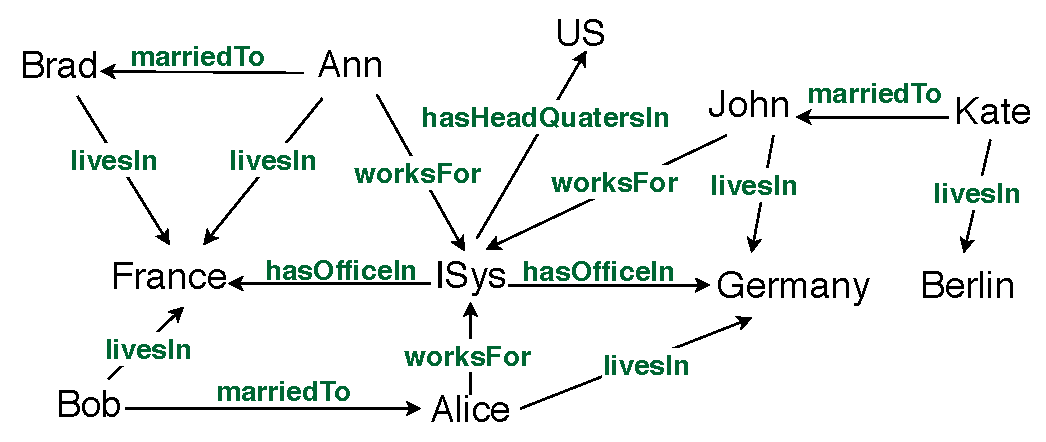
\includegraphics[width=0.8\textwidth]{figures/kg3.pdf}
%%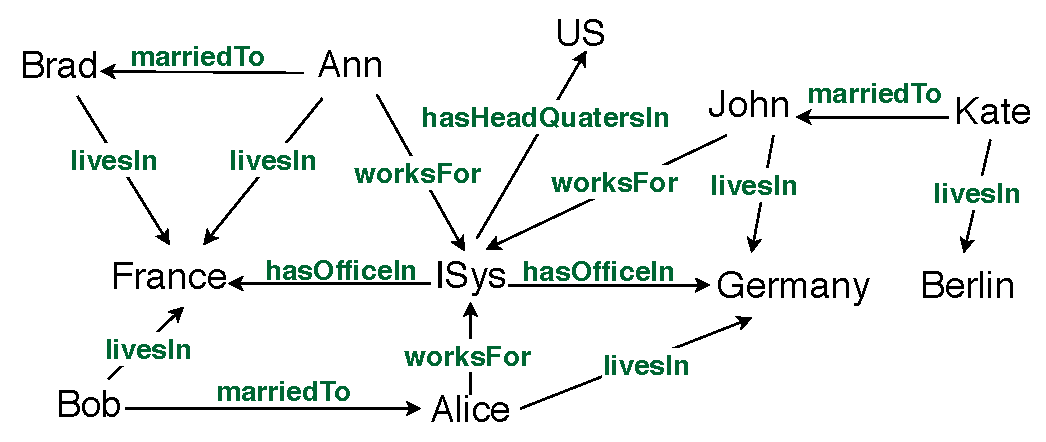
\includegraphics[scale=0.32]{figures/kg3.pdf}
%\caption{An example of a knowledge graph.}
%\label{fig:kg}
%\end{figure}

\section{Relational Association Rule Learning}
Association rule learning concerns the discovery of frequent patterns in a data set and the subsequent transformation of these patterns into rules.
A \emph{conjunctive query} over $\cG$ is of the form $Q(\vec{X}) \text{ :- } p_1(\vec{X_1}),\dotsc,p_m(\vec{X_m})$, where $\vec{X_i}$ are binary or unary vectors of variables and/or constants. Its  right-hand side (i.e., body) is a finite set of atomic formulas over $\Sigma_{\cG}$, while the left-hand side (i.e., head) is a tuple of variables occurring in the body and/or constants. The \emph{answer} of $Q$ on $\cG$ is the set $Q(\cG) = \{ \nu(\vec{X}) \mid \nu \text{ is a function from variables to } \mathcal{C} \text{ and } \forall i: p_i(\nu(\vec{X_i})) \in \cG \}$.
%As in \cite{DBLP:conf/ilp/DehaspeR97}, t
The \emph{support} of
$Q$ in $\cG$ is the number of distinct tuples in the answer of $Q$ on $\cG$. 
\begin{example}
\label{ex:ass_query_support}
The support of the following query:
\[Q(X,Y,Z) \text{ :- } worksFor(X,Y), hasOfficeIn(Y,Z)\]
over the KG $\cG$ in Fig. \ref{fig:kg} asking for people, their companies and the companies' locations is 12. \qed
\end{example}
An \emph{association rule} is of the form $Q_1 \Rightarrow  Q_2$, such that $Q_1$ and $Q_2$ are both conjunctive queries and $Q_1 \subseteq Q_2$, i.e., $Q_1(\cG')\subseteq Q_2(\cG')$ for any possible KG $\cG'$. In this work we exploit association rules for reasoning purposes, and thus (with some abuse of notation) treat them as logical rules, i.e., for $Q_1\Rightarrow Q_2$ we write $Q_2\backslash Q_1 \leftarrow Q_1$, where $Q_2 \backslash Q_1$ refers to the set difference between $Q_2$ and $Q_1$ seen as sets of atoms.
\begin{example}
Consider the query $Q$ from Example \ref{ex:ass_query_support} and also the following query:
\[Q'(X,Y,Z) \text{ :- } worksFor(X,Y), hasOfficeIn(Y,Z), livesIn(X,Z)\]
the \textit{association rule} $Q \Rightarrow Q'$ can be written as the following logical rule:\[livesIn(X,Z) \leftarrow worksFor(X,Y), hasOfficeIn(Y,Z)\]\qed
\end{example}

\begin{figure}[t]
\centering
\begin{tikzpicture}[->,>=stealth',auto,node distance=3cm,
  thick,main node/.style={font=\bfseries}]

  \node[main node] (1) {Brad};
  \node[main node] (2) [right=3cm of 1] {Ann};
  \node[main node] (3) [right=7.5cm of 1] {US};
  \node[main node] (5) [right=11cm of 1] {Kate};  
  \node[main node] (6) [below right =1.5cm and 0.75cm of 1] {France};
  \node[main node] (4) [right=7cm of 6] {John};  
  \node[main node] (7) [right=3cm of 6] {ISys};

  \node[main node] (10) [below left=1.5cm and 1cm of 6] {Bob};  
    \node[main node] (9) [right=11cm of 10] {Berlin};  
  \node[main node] (11) [right=3cm of 10] {Alice};  
  \node[main node] (8) [right=3cm of 11] {Germany};  
  
  \path[every node/.style={color=teal,fill=white,font=\small}]
    (2) edge node [right=-23pt] {\textit{marriedTo}} (1)
    (5) edge node [right=-30pt] {\textit{marriedTo}} (4)
    (10) edge node [right=-27pt] {\textit{marriedTo}} (11)    
    (1) edge node [right=-20pt] {\textit{livesIn}} (6)
    (2) edge node [right=-20pt] {\textit{livesIn}} (6)
    (5) edge node [right=-20pt] {\textit{livesIn}} (9)
    (4) edge node [right=-20pt] {\textit{livesIn}} (8)
    (11) edge node [right=-20pt] {\textit{livesIn}} (8)
    (10) edge node [right=-20pt] {\textit{livesIn}} (6)
    (2) edge node [right=-23pt] {\textit{worksFor}} (7)
    (4) edge node [right=-23pt] {\textit{worksFor}} (7)
    (11) edge node [right=-25pt] {\textit{worksFor}} (7)
    (7) edge node [right=-23pt] {\textit{hasOfficeIn}} (6)
    (7) edge node [right=-25pt] {\textit{hasOfficeIn}} (8)
    (7) edge node [right=-38pt] {\textit{hasHeadQuatersIn}} (3);
\end{tikzpicture}
\caption{An example knowledge graph.}
\label{fig:kg}
\end{figure}

\subsection{Rule Types}
Below we recap various rule types.
\begin{definition}[Connected rule] A rule is \textit{connected} if any two of its variables are connected through a series of atoms, where two atoms are connected if they share a variable or constant.
\end{definition}
\begin{example}
The rule below is connected:
\[isMusician(X) \leftarrow playsForBand(X, Y)\]
because variables X and Y are connected through the atom $playsForBand(X, Y)$. In contrast, the following rule is \textbf{not} connected:
\[speaks(X, English) \leftarrow livesIn(X, UK), worksIn(Y, US)\]
This rule seems to be meaningless, since there is no connection between $X$ and $Y$. If we remove the last atom $worksIn(Y, US)$, then the rule becomes connected. 
\qed
\end{example}
\begin{definition}[Closed rule] A \textit{closed} rule is a connected rule, whose every variable appears at least twice.
\end{definition}
\begin{example}
Rules $r_1$ and $r_2$ from Equations \ref{eq:ex-rule-1} and \ref{eq:ex-rule-2} are closed. An example of a non-closed rule is: \[musician(X) \leftarrow playsInstrument(X, Y)\]\qed
\end{example}

\begin{definition}[Recursive rule] A rule is called \textit{recursive} if its body contains the head predicate, since. Applying a recursive rule on the knowledge graph many times might predict new more facts.
\begin{example}
The rule $r_2$ is a recursive rule. In contrast, $r_1$ is \textbf{not} recursive, because the head predicate "livesIn" does not appear in the rule body. \qed
\end{example}

\end{definition}
\begin{definition}[Safe rule] A rule is \textit{safe} if every variable in its negated part appears in the positive part of the rule. %In other words, a rule is safe iff it is \textit{connected} and its Horn part is \textit{closed}.
\end{definition}
\begin{example}
The rule $r_3$ in Equation \ref{eq:ex-rule-3} is $safe$. In contrast, the following rule is unsafe:\[livesIn(Y,Z) \leftarrow marriedTo(X,Y), livesIn(X,Z), \naf doResearchAt(Y,T)\]
because variable T does not appear in the positive part of the rule.\qed
\end{example}
\subsection{Rule Statistics}
To quantify the quality of association rules on the knowledge graph, various rule metrics have been proposed. We list some prominent metrics below. Given a KG $\cG$, a rule $r : H \leftarrow B, \naf E$, where $H = h(X,Y)$ and $B,E$ involve variables from $\vec{Z}\supseteq \{X,Y\}$, the following measures can be computed:\\
- \textbf{Rule support} (or \textit{support}): indicates the absolute number of instantiations of a rule that are true in the knowledge graph.
\begin{equation}\label{eq:supp}
\textit{supp}(r,\cG) = \#(X,Y): H \in \cG, \exists \vec{Z}:B\in \cG,E \not \in \cG\\
\end{equation}
where $\# \beta : \mathcal{B}$ denotes the number of $\beta$ that fulfill the condition $\mathcal{B}$.\\
- \textbf{Body support}: indicates the absolute number of instantiations of rule's body in the knowledge graph.
\begin{equation}\label{eq:body_supp}
\textit{b-supp}(r,\cG) = \#(X,Y):\exists \vec{Z}:B\in \cG, E \not \in \cG
\end{equation}
- \textbf{Head support}: indicates the absolute number of instantiations of rule's head in the knowledge graph. In other words, this is the total number of facts in the KG over the head predicate $h$.
\begin{equation}\label{eq:head_supp}
\textit{h-supp}(r,\cG) = \#(X,Y): H \in \cG
\end{equation}
\begin{example}
Consider the two rules $r_1$, $r_2$ from Equations~\ref{eq:ex-rule-1} and \ref{eq:ex-rule-2} and the KG $\cG$ from Fig. \ref{fig:kg}. For the rule $r_1$, we have $supp(r_1,\cG)=3$ and $\textit{b-supp}(r_1,\cG) = 6$. Similarly, for $r_2$, we have $supp(r_2,\cG)=1$ and $\textit{b-supp}(r_2,\cG) = 3$. Moreover, $\textit{h-supp}(r_1,\cG) = \textit{h-supp}(r_2,\cG) = 6$, since there are totally 6 facts in $\cG$ with the head predicate $"livesIn"$.
\qed
\end{example}
\noindent- \textbf{Head coverage}: While support gives us the absolute number of correct rule instantiations, it does not tell us how much the rule affects the knowledge graph, since it does not take into account the size of the knowledge graph. Head coverage fixes this issue by reflecting the ratio of the rule support to the head support.
\begin{equation}\label{eq:hc}
\textit{hc}(r,\cG) = \frac{supp(r,\cG)}{\textit{h-supp}(r,\cG)}
\end{equation}
\begin{example}
We have $hc(r_1,\cG) = \frac{3}{6}$ and $hc(r_2,\cG) = \frac{1}{6}$.
\qed
\end{example}

\noindent- \textbf{Standard Confidence} (or \textit{confidence}): treats the knowledge graph under the Closed World Assumption (CWA). The standard confidence returns a number between $[0,1]$, which corresponds to the ratio of the rule support to the body support. Formally:
\begin{equation}\label{ex:m}
\mi{conf}(r,\cG) = \frac{\mi{supp}(r,\cG)}{\textit{b-supp}(r,\cG)}
\end{equation}
\begin{example}
We have $conf(r_1,\cG) = \frac{3}{6}$ and $conf(r_2,\cG) = \frac{1}{3}$. Moreover, for the following rule with negation:
\[\mi{r_4:\,livesIn(Y,Z) \leftarrow marriedTo(X,Y), livesIn(X,Z), not\;researcher(X)}\]
states that married people live together unless one is a researcher, 
and $\cG'=\cG\cup\{\mi{researcher(Bob)}\}$, we have $\mi{conf(r_4,\cG') = \frac{1}{2}}$.\qed
\end{example}
\noindent- \textbf{PCA Confidence} \cite{amie}: is based on the Partial Closed-world Assumption (PCA), which assumes that the data of the knowledge graph is added in batches. More specifically, for each subject $s$ and relation $p$, if there exists some object $o'$ such that $p(s,o') \in \cG$, then all possible true triples $p(s,o)$ are assumed to be presented in $\cG$. The \textit{PCA confidence} is defined as follows:
\begin{equation}\label{eq:pca_conf}
\mi{conf_{pca}}(r, \cG) = \frac{\textit{supp}(r, \cG)}{\#(X,Y): \exists \vec{Z}: B \in \cG, E \notin \cG  \wedge \exists Y': h(X,Y')\in \cG}
\end{equation}
Similar to the \textit{standard confidence}, the \textit{PCA confidence} also gives us a value between $[0,1]$.
\begin{example}
We have $conf_{pca}(r_1,\cG) = \frac{3}{6}$, $conf_{pca}(r_2,\cG) = \frac{1}{3}$ and $conf_{pca}(r_4,\cG') = \frac{1}{2}$. If Alice was not known to live in Germany in $\cG$, then $\mi{conf_{pca}(r_2,\cG)}=\frac{1}{2}$. \qed
\end{example}

\noindent- \textbf{Conviction} \cite{trantowards}: is shown to correlate with the rule predictive power \cite{Azevedo2007}.
%by measuring the intensity of rule's implication \cite{DBLP:conf/eurogp/MinhdNT18}
\textit{Conviction} is defined as follows:
\begin{equation}\label{eq:conv}
\textit{conv}(r,\cG) = \frac{1 - \textit{rel-supp}(h, \cG)}{1-\textit{conf}(r,\cG)}
\end{equation}
where $\textit{rel-supp}(h)$ is the relative support of the head, which is measured by:
\begin{equation}
\textit{rel-supp}(h, \cG) = \frac{\textit{h-supp}(r,\cG)}{(\# X: \exists Y' :h(X,Y') \in \cG) \times (\#Y :\exists X': h(X',Y) \in \cG)}
\end{equation}
\begin{example}
We have $\textit{rel-supp}(livesIn, \cG) = \frac{6}{6 \times 3} = \frac{1}{3}$. Thus, $conv(r_1,\cG) = \frac{1 - \frac{1}{3}}{1 - \frac{3}{6}} = \frac{4}{3}$ and $conv(r_2,\cG) = \frac{1 - \frac{1}{3}}{1 - \frac{1}{3}} = 1$.
\qed
\end{example}
Unlike standard confidence and PCA confidence, conviction gives us a value in $[0,\infty]$.
\subsection{Rule-based KG Completion}

Given a rule $r$ and a KG $\cG$ the application of $r$ on $\cG$ results in a rule-based graph completion defined relying on the answer set semantics as recapped in Section \ref{sec:non-prog}.

\begin{definition}[Rule-based KG completion]\label{def:graphcompl}
Let $\cG$ be a KG over the signature $\Sigma_{\cG}=\tuple{\mathbf{R},\cC}$ and let $r$ be a rule %$r$ be a set of rules 
mined from $\cG$, i.e. a rule over $\Sigma_{\cG}$.
Then the \emph{completion of $\cG$} using $r$ is a graph $\cG_{r}$ constructed from any answer set of $r \cup \cG$. 
\end{definition}

\begin{example}
The application of $r_1$ and $r_2$ on $\cG$ from Figure \ref{fig:kg} results respectively in:\\
\textit{ - $\cG_{r_1} = \cG\;\cup$ \{livesIn(Ann,Germany), livesIn(John,France), livesIn(Alice,France)\}}\\
\textit{ - $\cG_{r_2} = \cG\;\cup$ \{livesIn(Alice,France), livesIn(John, Berlin)\}}. \qed
\end{example}

Note that $\cG^i$ is the perfect completion of $\cG$, i.e., it is supposed to contain all
correct facts with entities and relations from $\Sigma_{\cG}$ that hold
in the current state of the world. The goal of the rule-based KG completion is to extract from $\cG$ a set of rules $\cR$ such that $\cG_{\cR} = \cup_{r\in \cR}\cG_{r}$ is as close to $ \cG^i$ as possible.

\section{Link Prediction Embedding Models} 
Recently a vast amount of latent-based approaches for statistical relational learning have been proposed  (see \cite{Nickel0TG16} for overview), which address the KG completion problem by reducing it to a representation learning task, where the main goal is to represent entities and relations of $\cG$ in a
low-dimensional, say $d$-dimensional, vector (aka embedding) and relying on these representation estimate the likelihood (not necessary probability) of the potentially missing facts. 
%vector space $\vec{h}, \vec{t}, \vec{r} \in I\!R^d$ such that for $\tuple{h,r,r}\in \cG$ it holds that $\vec{h}+\vec{r}\approx \vec{t}$.  
Some models rely exclusively on the triples in the available graph and estimate the likelihood of the missing ones~\cite{Bordes:NIPS2013,DBLP:conf/aaai/NickelRP16}, while others may utilize external resources (\eg text)~\cite{DBLP:conf/aaai/0005HMZ17}. 

%For a pair $\tuple{\cG, \cE}$, $\cE$ is an embedding model of $\cG$, if for each triple $\tuple{s,p,o}\in \cG$, there exists a vector $v \in \cE$. 
Typical embedding models define a scoring function $\xi: \cR_\cG \times \cC_\cG \times \cC_\cG \rightarrow \mathbb{R}$ that given an $\tuple{\mi{s,p,o}}$ triple computes a numerical value reflecting its likelihood. The higher score is, the more plausible the triple is. While in this work we experiment with several selected KG embedding models, our general rule learning approach can conceptually exploit any model. Some prominent embedding models have been recapped in related work of Chapter \ref{sec:related-work}.

%If we treat a KG embedding model as an oracle, then the questions that one can pose to it include $\tuple{s,p,o}$, $\tuple{s,p,?}$, $\tuple{?,p,o}$ and $\tuple{s,?,o}$. Apart from asking for the plausibility score of an individual fact $\tuple{s,p,o}$, the existing embedding models can also output a list of ordered potentially missing objects given a $\tuple{s,p,?}$ by ranking them based on the plausibility score. Other two types of queries that can be posed to an embedding model including $\tuple{?,p,o}$ and $\tuple{s,?,o}$ could be treated similarly.




%!TEX root = ../main.tex

%!TEX root = ../main.tex


\chapter{Rule Learning Guided by External Sources}
\label{sec:framework}
%---------------------------------------------------------%

In this chapter, we introduce our framework for rule learning guided by external sources,
discuss challenges associated with it, and finally propose its concrete instantiation with embedding models.

%\section{Background}
%%---------------------------------------------------------%
%
%We assume countable sets $\mathcal{R}$ of unary and binary relation names and $\mathcal{C}$  of constants. 
%A \emph{knowledge graph} (KG) $\G$ is a finite set of ground atoms $a$ of the form
%$P(b,c)$ and $C(b)$ over %the 
%$\R\cup\C$.
%With $\Sigma_{\cG}$, the \emph{signature} of $\G$, we denote elements of $\R\cup\C$ that occur in $\G$.\looseness=-1
%
%
%We define rules over KGs following the standard approach of non-monotonic logic programs under the answer set semantics %, see e.g. 
%\cite{GL1988}.
%Let $\X$ be a countable set of variables.
%A \emph{rule} $r$ is %an expression 
%of the form
%$
%\mi{head \leftarrow body},
%$
%where $\mi{head}$, or $\mi{head}(r)$, is an atom 
%%of the form $a(\vec{X})$ 
%over $\R\cup\C\cup\X$ 
%%and $\vec{X}$ are its variables,
%and $body$, or $\mi{body}(r)$, is a conjunction of positive and negative atoms 
%over $\R\cup\C\cup\X$.
%Finally, 
%$\mi{body^+(r)}$ and $\mi{body^-(r)}$ denote the atoms that occur in $\mi{body(r)}$ positively and negatively respectively, that is, the rule can be written as
%$
%\mi{head(r) \leftarrow body^+(r), not\ body^-(r)}.
%$
%A rule is \emph{Horn}, if all head variables occur in the body,
%and $\mi{body^-(r)}$ is empty.
%
%
%We define \emph{execution} of rules with default negation~\cite{GL1988} over KGs in the standard way.
%More precisely, let $\G$ be a KG, $r$ a rule over $\Sigma_\G$, 
%and $a$ be an atom over $\Sigma_\G$.
%Then, $r \models_\G a$ holds if there is a variable assignment that maps atoms $\mi{body^+(r)}$ in $\G$ such that it does not map any of the atoms in $\mi{body^-(r)}$ in $\G$. 
%Then, let $\G_r = \G \cup \set{a \mid r \models_\G a}$. 
%Intuitively, $\G_r$ extends $\G$ with edges derived from $\G$ by applying $r$.

\section{Problem Statement and Proposal of General Solution} 
%---------------------------------------------------------%
Let $\G$ be a KG over the signature $\Sigma_{\G}=\tuple{\cR_\G,\cC_\G}$. 
A \emph{probabilistic KG} $\PG$ is a pair $\PG = (\G,f)$ 
where $f:\cR_\G\times \cC_\G \times \cC_\G\rightarrow [0,1]$ is a probability function over the facts over $\Sigma_{\G}$ such that for each atom $a \in \G $ it holds that $f(a) = 1$.

The goal of our work is to learn rules that not only describe the available graph $\cG$ well, but also predict highly probable facts based on the function $f$.
The key questions now are how to define the quality of a given rule $r$ based on $\PG$ and how to exploit this quality during rule learning for pruning out not promising rules. 

% Let $\G_r = \G \cup \set{a \mid r \models_\G a}$, where $r$ is a rule mined from $\G$.
% Intuitively, $\G_r$ extends $\G$ with edges derived from $\G$ by applying $r$.
% The set $\G_r \setminus \G$ denotes all facts that may be present
% in the %real
% ideal KG, but are missing in the incomplete $\G$, and $f$ gives the probability of these facts.

A quality measure $\mu$ for rules over probabilistic KGs 
is a function $\mu: (r,\PG) \mapsto \alpha$, where $\alpha \in  [0,1]$.
In order to measure the quality $\mu$ of $r$ over $\PG$ we propose: 
\begin{itemize}
\item 
to measure the quality $\mu_1$ of $r$ over $\G$, where $\mu_1: (r,\cG) \mapsto \alpha \in  [0,1]$,
\item
to measure the quality $\mu_2$ of $\G_r$ by relying on $\PG_r=(\cG_r,f)$, 
where $\mu_2{:}\, (\G'{,}\, (\G,f)) \mapsto  \alpha \,{\in}\, [0,1]$ for $\G' \supseteq \G$ is the quality of extensions $\G'$ of $\G$ over $\Sigma_\G$ given $f$,
and 
\item
to combine the result as the weighted sum.
\end{itemize}
That is, we define our hybrid rule quality function $\mu(r,\PG)$ as follows:
\begin{align}\label{eq:hm}
	\mu(r,\PG)= (1 - \lambda)\times \mu_1(r,\cG) + \lambda \times \mu_2(\G_r,\PG).
\end{align}
In this formula $\mu_1$ can be any classical quality measure of rules over complete graphs. %  and 
% $\mu_2$ 
% \thi{mu2 what?}.
Intuitively, $\mu_2(\G_r,\PG)$ is the quality of $\G_r$ wrt $f$ that allows us to capture the information about facts missing in $\G$ that are relevant for $r$.
The weighting factor %parameter 
$\lambda$, we call it \textit{embedding weight}, allows one to choose whether %one prefers 
to rely more on the classical measure $\mu_1$ or on the measure $\mu_2$ of the quality of the facts that 
are predicted by $r$ over $\G$.

\subsection{Challenges} 
%---------------------------------------%
There are several challenges that one has to face when realizing our approach:
\begin{itemize}
\item First, given an incomplete KG $\G$, one has to define $f$
such that $(\G,f)$ satisfies the expectations, i.e., reflects well the probabilities of missing facts.
\item Second, one has to define $\mu_1$ and $\mu_2$ that also satisfy the expectations and admit efficient implementation.
\item Third, the adaptation of existing rule learning approaches to account for the probabilistic function $f$ without the loss of scalability is not trivial. 
Indeed, materializing $f$ by augmenting $\cG$ with all possible probabilistic facts over $\Sigma_{\cG}$ and subsequently applying standard rule learning methods on the obtained graph is not practical. Storing such potentially enormous augmented graph 
where many probabilistic facts are irrelevant for the extraction of meaningful rules might be simply infeasible.
\end{itemize}
%\looseness=-1
\section{Realization of General Solution}
\label{section: realisation}
%------------------------------------------------------------%
We now %present 
describe how we addressed the above stated challenges in this thesis.
In Section~\ref{section: realisation} we present concrete realizations of $f$, $\mu_1$ and $\mu_2$, and in Section~\ref{sec:sys} we discuss how we implemented them and adapted within an %rule learning as an 
end-to-end rule learning system.

% In what follows we present our solution to the above challenges by discussing the realizations of $f$, $\mu_1$ and $\mu_2$, and in Section~\ref{sec:sys} present the end-to-end rule learning systems that exploits our proposals.

\subsection{Realization of the Probabilistic Function $f$}
%------------------------------------------------------------%
We propose to define $f$ by relying on embeddings of KGs.
Embedding models can be used to estimate the likelihood of potentially missing binary atoms
using a scoring function $\mi{\xi: \cR_\cG \times \cC_\cG \times \cC_\cG \rightarrow \mathbb{R}}$.
Examples of concrete scoring functions can be found, e.g., in~\cite{DBLP:journals/tkde/WangMWG17}.
Since embeddings per se are not in the focus of this thesis,
we will not give further details on them and refer the reader to~\cite{DBLP:journals/tkde/WangMWG17} for an overview.
Note that our framework is not dependent on a concrete embedding model. 
What is important for us is that embeddings can be used to construct probabilistic representations~\cite{DBLP:conf/aaai/NickelRP16} of atoms missing in KGs and we use this to define $f$.

Consider an auxiliary definition. Given a KG $\G$, and an atom $a=p(s,o)$, the set $\G_s$ consists of $a$ and all atoms $a'$ that are obtained from $a$ by replacing $s$ with a constant from $\Sigma_\G$, except for those that are already in $\G$. 
Then, given a scoring function $\xi$, $[\G_s]$ is a list of atoms from $\G_s$ ordered in the descending order.
Finally, the \emph{subject rank}~\cite{DBLP:journals/corr/abs-1301-3485} of $a$ given $\xi$, $\mi{subject\_rank_\xi(a)}$ is the position of $a$ in $[\G_s]$. 
Analogously one can define $[\G_o]$ and the corresponding 
\emph{object rank}~\cite{DBLP:journals/corr/abs-1301-3485} of $a$ given $\xi$, that is, $\mi{object\_rank_\xi(a)}$. 

Now we are ready to define the function $f$ for an atom $a$ %:it i
as the average of its subject and object inverted ranks given $\xi$~\cite{DBLP:journals/corr/abs-1301-3485}, i.e.:
\begin{align}
\label{eq:f}
\mi{f_\xi(a)} = 0.5\times(1/\mi{subject\_rank_\xi(a)}+ 1/\mi{object\_rank_\xi(a)})
\end{align}



\subsection{Realization of $\mu_1$}
%---------------------------------------------------%
This measure should reflect the descriptive quality of a given rule $r$ with respect to $\cG$.
There are many classical data mining measures that can be used as $\mu_1$, see, e.g. \cite{DBLP:conf/eurogp/MinhdNT18,amie,carl,measureskg} for $\mu_1$s proposed specifically for KGs. In principle, we should choose a suitable measure that correctly describes the KG.

In our work we selected the following two measures for $\mu_1$:
\emph{standard confidence} and \emph{PCA confidence}. While standard confidence of a rule is the conditional probability of rule's head given its body, computed based on closed world assumption (CWA), PCA confidence is its generalisation to the open world assumption (OWA), which does not penalize rules that predict facts $p(s,o)$, such that $p(s,o')\not \in \cG$ for any $o'$. 

\subsection{Realization of $\mu_2$}
%---------------------------------------------------%
There are various ways how one can define the quality $\mu_2(\G_r,\PG)$ of $\G_r$.
A natural candidate to define the quality of $\G_r$ is the probability of $\G_r$, that is, as
$\mu_2(\G_r,\PG)=\prod_{a \in \G_r} f(a) \times \prod_{a \in (\R_\G\times\C_\G\times\C_\G)\setminus \G_r} (1-f(a))$.
A disadvantage of such quality measure is that in practice it will be very low,
as the product of many (potentially) small probabilities,
and thus Equation~\ref{eq:hm} will be heavily dominated by $\mu_1(r,\cG)$. Therefore,
we advocate 
%foranother proposal: 
to define $\mu_2(\G_r,\PG)$ as %the 
the average probability of newly predicted facts in $\G_r$:
\begin{align}
	\mu_2(\G_r,\PG) = (\Sigma_{a\in \cG_r\backslash \cG} f(a)) /
				|\cG_r \backslash \cG|.
\end{align}

\begin{example}\label{ex:hm}
Consider the KG $\cG$ in Figure~\ref{fig:kg}, and the rules from Equations~\ref{eq:ex-rule-1} and \ref{eq:ex-rule-2} with their confidence values as presented in Example~\ref{ex:m}. Suppose that a text-enhanced embedding model produced a relatively accurate estimation of the probabilities of facts over $\mi{livesIn}$ relation. For example, even though within the graph there is no direct connection between Germany and Berlin, relying on the living places of entities similar to John and hidden semantic relations between Germany and Berlin such as co-occurrences in text and other linguistic features, for the fact $\mi{a=livesIn(john,berlin)}$ we obtained $f(a)=0.9$, while for $a'=\mi{livesIn(john,france)}$, a much lower probability $f(a')=0.09$. These naturally support the predictions of $r_2$ but not those of $r_1$.

Generalising this idea, assume that on the whole dataset we get $\mi{\mu_2(\cG_{r_1},\PG)}=0.1$ and $\mi{\mu_2(\cG_{r_2},\PG)=0.8}$, where $\PG=(\cG,f)$. Thus, for $\lambda=0.5$ we have $\mu(r_1,\PG)=(1-0.5)\times 0.5+0.5\times 0.1 = 0.3$, while for $\mu(r_2,\PG)=(1-0.5) \times \frac{1}{3}+0.5\times 0.8\approx 0.57$, resulting in the desired ranking of $r_2$ over $r_1$ based on $\mu$.
%\ds{Maybe we should shift this discussion to methodology?}
\qed 
\end{example}

\section{Approach Overview} 
\label{sec:sys}
%-------------------------------------------%

In this section, we present the main phases of our approach. 
Conceptually, our system generalizes the standard relational association rule learners \cite{amie,DBLP:conf/esf/GoethalsB02} to account for the feedback from the probabilistic function $f$. 
Following common practice~\cite{amie} we restrict ourselves to rules that are \emph{closed} and \emph{safe}.

\begin{figure}[t]
\centering
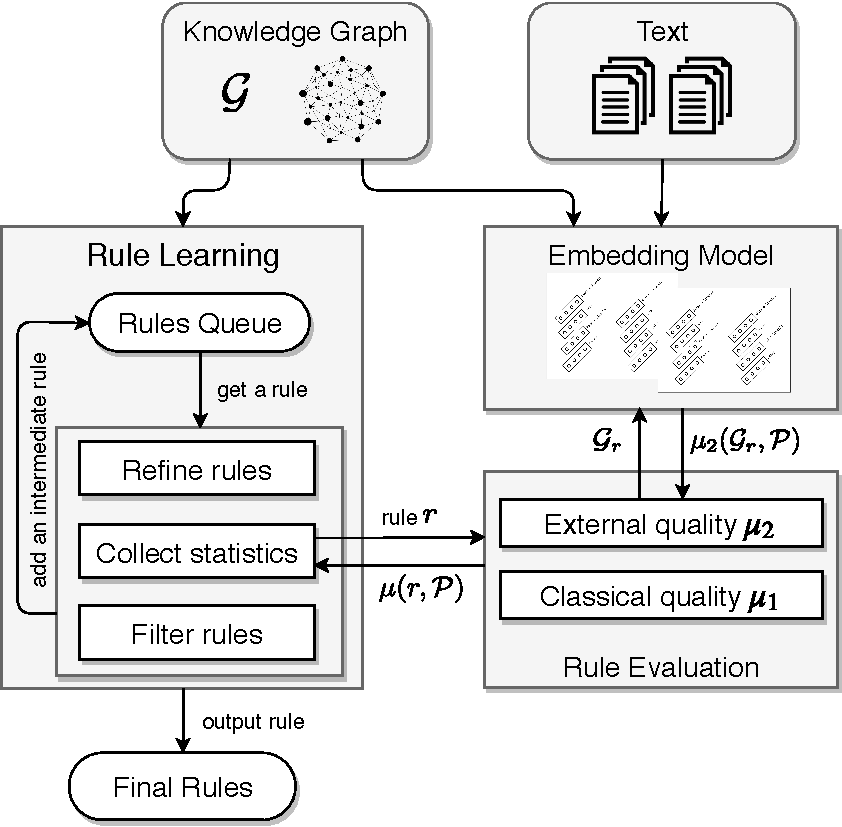
\includegraphics[width=0.7\textwidth]{figures/system_overview_V.pdf}
\caption{Overview of our system.}\label{fig:system}
\end{figure}

%------------------------------------------%
The input of the system are a KG, possibly a text corpus, and a set of user specified parameters that are used to terminate rule construction.
These parameters include an embedding weight $\lambda$, 
a minimum threshold %$\mi{\mu_1\_min}$ 
for $\mu_1$,  
a minimum rule support $\textit{r-supp}$ %(r,\cG)$ 
and other \emph{rule-related} parameters such as a maximum number of positive %$\mi{max\_pos}$ 
and negative %$\mi{max\_neg}$ 
atoms allowed in $\mi{body(r)}$.
The KG and text corpus are used to train the embedding model that in turn is used to construct the probabilistic function $f$.
The rules $r$ are constructed in the iterative fashion, starting from the head, by adding atoms to its body one after another until at least one of the termination criteria (that depend on $f$) is met.
In parallel with the construction of $r$ the quality $\mu(r)$ is computed.

In Figure~\ref{fig:system}, we present a high level overview of our approach, where arrows depict information flow between blocks.
The \emph{Rule Learning} block constructs rules over the input KG, \emph{Rule Evaluation} supplies it with quality scores $\mu$ for rules $r$, using $\cG$ and $f$, where $f$ is computed by the \emph{Embedding Model} block from $\cG$ and text. Below, we describe in more detail each of these components in our system.

\subsection{Embedding Model} 
Embedding model is the key component that is used to measure the external quality $\mu_2$ of the rules. For the basic operation, embedding model gives each given a fact $p(s,o)$ a numerical value reflecting its likelihood. This component is pre-trained on the available KG and possibily with external data (e.g. texts), depending on the chosen model. Some prominent embedding models have been briefly described in chapter \ref{sec:related-work}.

\subsection{Rule Learning} 
\begin{algorithm}[t]
\DontPrintSemicolon
$queue\leftarrow \langle[]\rangle$\\
Execute in parallel:\\
\While{$\neg$queue.isEmpty()}{    
    \textit{rule $\leftarrow$ queue.dequeue()}\\
    \tcc{Computes rule statistics and output if necessary.}
    \If{rule.isClosed()}{
        \textit{stats $\leftarrow$ computeStatistics(rule)}\\
        \eIf{stats is not pruned for outputting}{
            output($rule$)
        }{
            continue while loop
        }
    }
    \tcc{Applies refinement operators to explore more new rules.}
    \ForEach{operator o}{
        \ForEach{newRule $\in$ o(rule)}{
            \If{newRule satisfies language bias}{
                \tcc{Checks if there is some version of rule in queue.}
                \If{newRule $\notin$ queue}{ 
                    \textit{queue.enqueue(newRule)}
                }
            }
        }
    }    
}
\caption{(Non-)monotonic Rule Mining}
\label{algor:mining}
\end{algorithm}

%\subsection{Rule Learning}
%\cm{maybe seperate to blocks talking about overview}

Algorithm \ref{algor:mining} demonstrates the mining process behind the \emph{Rule Learning} block in Figure~\ref{fig:system}, in which we will discuss now. Following \cite{amie} we model rules as sequences of atoms, where the first atom is the head of the rule and other atoms are its body. The algorithm maintains a (priority) queue of intermediate rules (see the \emph{Rules Queue} component in Figure~\ref{fig:system}). 
%Initially all possible binary atoms appearing in $\cG$ are added to the queue with empty bodies.
Initially the queue contains only an empty rule. At each iteration, a single rule is selected from the queue for processing. If the rule satisfies the \emph{filtering criteria} (\emph{Filter rules} in Fig. \ref{fig:system}) which we define below, then the system returns it as an output. If the rule is not filtered, then it is processed with one of the \emph{refinement operators} (\emph{Refine rules} in Fig. \ref{fig:system}) 
that we define below that expand the rule with one more atom and produce new rule candidates, which are then pushed into the queue (if not being pushed before). The iterative process is repeated until the queue is empty. All the reported rules are finally ranked by the decreasing order of the hybrid measure $\mu$, computed in \emph{Collect statistics} block.

In the remainder of this section, we discuss refinement operators, filtering criteria, and how to check rule duplication efficiently.

\subsubsection{Refinement Operators}
%------------------------------------------%
We rely on the following three standard refinement operators \cite{amie}
that extend rules:
\begin{enumerate}
\item[\it (i)] \textit{add a positive dangling atom}: add a new positive atom with one fresh variable and another one appearing in the rule, i.e., \emph{shared}.
\item[\it (ii)] \textit{add a positive instantiated atom}: add a positive atom with one argument being a constant and the other one being a shared variable.
\item[\it (iii)] \textit{add a positive closing atom}: add a positive atom with both of its arguments being shared variables.
\end{enumerate}

Additionally, we introduce two more operators to allow negated atoms in rule bodies: 

\begin{enumerate}
\item[\it (iv)] \textit{add an exception instantiated atom}: add a negated atom with one of its arguments being a constant, and the other one being a shared variable. 
%Note that as usual we model unary atoms (e.g., $person(x)$) as instantiated binary atoms (e.g., $type(x,person)$).
\item[\it (v)] \textit{add an exception closing atom}: add a binary negated atom to the rule with both of its arguments being shared variables or a unary negated atom with a shared variable. 
\end{enumerate}
%
These two operators are only applied to \textit{closed} rules to ensure the \textit{safety} condition.
Moreover, we also require the satisfaction of the following condition:
for a rule \\$r:\mi{head(r)\leftarrow body^+(r)}$ the addition of an exception atom should result in the rule $r': \mi{head(r)\leftarrow body^+(r), body^-(r)}$, such that the following condition holds:
\begin{equation}
\mi{\textit{supp}(r,\cG)=\textit{supp}(r',\cG)}
\end{equation}
Intuitively, the application of exception refinement operators must not lead to the decrease of the rule support, i.e., exceptions should explain the absence of predictions expected to be in the graph rather then their presence.


\subsubsection{Filtering Criteria}
Without any filters and restrictions, we can theoretically explore all possible rules. However, most of them are useless for us. Hence, pruning strategies are needed to extract only meaningful rules as well as to enhance the performance of the algorithm. We classify these filtering criteria into 2 categories: \textit{language-bias-based-filters} and \textit{statistics-based-filters}.

\leanparagraph{- Language-bias-based Filtering}

After applying one of the refinement operators to a rule, 
a set of candidate rules is obtained. At this step, we can decide whether we should prune them by directly looking at their format.
Following other rule mining systems, we also aim at mining only \textit{closed} rules from the knowledge graphs. For rules having non-empty negated part $body^-(r)$, we allow only rules having closed positive part. Note that while non-closed rules are not returned in the output, they still be pushed into the rule queue to construct new rules, since a closed rule can be generated only by extending some other non-closed rule.

In addition, we also put some thresholds on the form of rules we want to extract from the knowledge graph, including:
\begin{itemize}
  \item Number of distinct variables appearing in rule. 
  \item Number of all atoms, positive atoms and negated atoms.
  \item Variable degree, which is the maximum number of atoms using the same variable as their arguments.
  \item Number of predicate occurrences in a rule.
\end{itemize}
All of the above restrictions are checked in line 13 of Algorithm \ref{algor:mining}. This ensures that all rules we push into the queue are exactly the ones we are interested in.

\leanparagraph{- Statistics-based Filtering}

%------------------------------------------%
Filtering by language bias only introduces restrictions on the form of rules to be extracted from the KG, without looking at the their quality. So, rules' statistics are collected by the \emph{Rule Evaluation} block in Figure~\ref{fig:system} (line 6 of Algorithm \ref{algor:mining}), and in line 7 of Algorithm \ref{algor:mining}, we filter the rules based on these statistical metrics as follows:

\noindent- \textit{Rule support}: Rules that have low support are likely to be noise, so we filter out all rules having support less than some minimum threshold.

\noindent- \textit{Head coverage}: Since we are not interested in rules that cover only a small portion of facts over the head predicate, following \cite{amie}, we prune out all rules having head coverage below some defined threshold.

\noindent- \textit{Classical quality $\mu_1$}: If the classical quality $\mu_1$ of the rule is too low, it is very likely that its external quality $\mu_2$ is likewise low, leading to a very low value of the hybrid quality $\mu$. Hence, we filter out all rules whose classical quality $\mu_1$ is below a defined threshold. Obviously, by filtering rules based on their quality, we not only get rid of nonpromising rules but also restrict the rule search space, thus improving the performance of the whole system. More specifically, since querying the embedding model for $\mu_2$ is a time-consuming operation, we only do this for rules whose $\mu_1$ is above a minimum value.

\noindent- \textit{Increasing hybrid quality}: For each candidate rule we check whether the application of refinement operators results in the increase of the hybrid measure $\mu$, and discard the rule otherwise.

\noindent- \textit{Exception confidence}: We propose the novel exception confidence measure, which is computed after the addition of an exception atom to a rule. Formally, given a rule of the form $r: head(r) \leftarrow body^+(r), \naf body^-(r)$, its exception confidence is computed as:
\begin{align}
	\textit{e-conf}(r,\cG) & = \textit{conf}(r',\cG)
\end{align}
where $r':body^-(r)\leftarrow body^+(r), not\;head(r)$. If the \emph{e-conf} is below some user specified threshold, then the rule is dropped.

Intuitively, exception confidence is the conditional probability of the exception given predictions produced by the Horn part of $r$, which helps to disregard insignificant exceptions, i.e., those that explain the absence in $\cG$ of only a small fraction of predictions made by $\mi{head(r)}\leftarrow \mi{body^+(r)}$, as such exceptions likely correspond to noise. Note that by exploiting the embedding feedback, we can now distinguish exceptions from noise. 
Consider the rule stating that married people live together. This rule can have several possible exceptions, e.g., either one of the spouses is a researcher or he/she works at a company, which has headquarter in the US. Whenever the rule is enriched with an exception, naturally, the support of its body decreases, i.e., the size of $\cG_r$ goes down. Ideally, we want to add such negated atoms, that the average quality of $\cG_r$ increases, as this will witness that by adding negated atoms to the rule we get rid of unlikely predictions. 

Observe that not all of the filtering criteria are relevant for all rule types. For example, exception confidence is relevant only for non-monotonic rules to ensure the quality of the added exceptions. Moreover, increasing hybrid quality is only used as a filtering criterion for closed rules. Indeed, if the rule is non-closed, this filter is not meaningful \cite{amie}.

\subsubsection{Checking Rule Duplication}
Since one rule could be generated multiple times from applying mining operators in different orders, and it does not make sense to process a rule more than once, we will prune all duplicated versions of the same rule. At line 14 of Algorithm \ref{algor:mining}, we push a rule into the queue only if none of its versions is already pushed in the queue. Because the queue contains rules in increasing order of the number of atoms, we can ensure that all duplicated versions of the same rule will be checked through this line of code before the first one of them is processed.

To check if twos rule are duplicated, we can check if there exists a bijection mapping variables between the two rules, such that the structure of the two rules with mapped variables are exactly the same. To check if a rule already exists in the queue, theoretically, we need to compare it with all other rules in the queue. However, we could reduce the number of rules to be compared with by using a hash table, where we encode each rule with a hash code in such a way that duplicated rules must have the same hash code. A good hash function should minimize the number of collisions (i.e. total number of different rules having the same hash code). There are many ways to define a hash code function. For example, we could exploit the number of variables, number of atoms of each type, number of atoms of each predicate, variables degree, graph structure of the rule, etc. An optimization to support the rule duplication checking process is to impose a constraint on the order of refinement operators to be applied on the rule.


\subsection{Rule Evaluation}
\label{rule:eva}
Another key component of our system is the \textit{Rule Evaluation}. Obviously, the question here is how to compute rule statistics. We now briefly describe how we answer this question.

For each rule $r: H \leftarrow B, \naf E$, where $H = h(X,Y)$ we need to calculate its statistics (e.g. head coverage $hc$, classical quality $\mu_1$, hybrid quality $\mu$, and possibly exception confidence $\textit{e-conf}$ if the rule is non-monotonic). The statistics computation involves a subtask of finding all instances of the head variables $(X,Y)$ satisfying the body of the rule. Then, head coverage can be derived by computing the ratio of the number of such pairs $(X,Y)$ satisfying the head of the rule (i.e. rule support) to the total head support. Standard confidence is calculated based on the ratio of rule support to the body support. External quality $\mu_2$ is computed by querying the embedding model. Other metrics can be derived accordingly.

\begin{algorithm}[t]
\DontPrintSemicolon
\SetKwInOut{Input}{Input}
\SetKwInOut{Output}{Output}
\SetKwProg{Fn}{Function}{}{}
\Input{Rule body $[B_1, B_2, ..., B_n]$ (may contains exceptions) with head variables $(X,Y)$}
\Output{Instances of ${(X,Y)}$}

\textit{ins $\leftarrow \{\}$} \texttt{// Stores instances of $(X,Y)$.}\\
\textit{val $\leftarrow$ array of null values} \texttt{// Stores variables assignments while backtracking.}\\
\Fn{FillAtom(bodyIndex)}{
\If{bodyIndex = n + 1}{
    $ins \leftarrow ins \cup \{(val[X], val[Y])\}$\\
    return
}
$atom \leftarrow B_{bodyIndex}$\\
$null\_atom\_variables \leftarrow \{variables\ v\ \in atom\ |\ val[v]\ is\ null\}$\\
\eIf{null\_atom\_variables is empty}{
    \eIf{val satisfies atom}{
        \textit{FillAtom(bodyIndex + 1)}
    }{
        return
    }
}{
    \ForEach{values of null\_atom\_variables that satisfy $[B_1, B_2, ..., B_{bodyIndex}]$}{
        $val[null\_atom\_variables] \leftarrow assigned\ values$\\
        \textit{FillAtom(bodyIndex + 1)}\\
        $val[null\_atom\_variables] \leftarrow null$
    }
}
}
\textit{FillAtom(1)}\\
return $ins$

\caption{Find Body Instances}
\label{algor:stats}
\end{algorithm}

Algorithm \ref{algor:stats} describes how we find the head instances $(X,Y)$ that satisfy the rule body. The general idea is to try recursively assigning constants $c \in \cC$ to variables to satisfy body atoms one by one. Once the current variables assignment cannot satisfy the given atom (line 12), we backtrack to the previous atom and assign different values to variables. For each variables assignment that satisfies all the body atoms, we insert the value of pair $(X,Y)$ into the result (line 5), which is an empty set at the beginning.

\subsubsection{Optimized Computation of External Rule Quality}
Clearly, computing the external rule quality $\mu_2$ is a heavy operation. Indeed, to compute $\mu_2$, we need to compute the probabilistic value $f$ for each fact predicted by the rule and take the average of them. Moreover, to calculate $f$ for a fact, one needs to calculate its \textit{subject rank}\cite{DBLP:journals/corr/abs-1301-3485} and \textit{object rank}\cite{DBLP:journals/corr/abs-1301-3485} by looping through all substitutions of subject and object with other entities and then querying the  embedding model for the likelihood scores $\xi$.

If the number entities and/or the number of facts predicted by the rule is high, which is very likely for modern KGs, then computing the value of $\mu_2$ is too time-consuming. So, a full implementation to compute $\mu_2$ will lead to a very poor performance of the mining algorithm. Below, we discuss possible optimizations to fix this issue.

\noindent- \textit{Facts sampling}: First, notice that the external quality function $\mu_2$ is defined as the average probability $f$ of rule predictions. Hence, the first thing we can do is to take a sample of the rule predictions and estimate their average probability $f$ based on this set. This solution would speed up the calculation of $\mu_2$ in the situation when a rule predicts a very large number of facts, which usually happens for low confidence rules on large knowledge graphs.

\noindent- \textit{Subject/Object ranks early stopping}: To compute the probability $f$ of a fact based on the Equation \ref{eq:f}, we need to compute its \textit{subject/object ranks}. It is easy to see that the value of $f$ does not change significantly when the subject/object ranks rise to a large enough value. Based on this observation, we can set thresholds on the maximum values of the subject and object ranks, and when looping through the substitutions of the subject/object, we will stop whenever the current subject/object ranks touch these thresholds.

\noindent- \textit{Caches for Embedding model}: Another relevant optimization for computing $\mu_2$ efficiently is to use caching for querying the likelihood scores $\xi$. While the time required for retrieving an answer of a query for computing $\xi$ depends on the choice of the embedding model as well as its hyper parameters, using a Least Recently Used (LRU) cache might be in any case helpful. In principle, we can even use multiple caches, i.e. a separate one for each KG relation.

\noindent- \textit{Optimized Embedding model}: The final optimization is at the calculation of the likelihood function $\xi$ alone. This advantageous optimization highly depends on the chosen embedding model and its likelihood formula. Not all models can be improved at this step, and to achieve reasonable enhancements, a deep understanding of the model is required. In our work, since we rely on available implementations of embedding models, this optimization is not applied.






\chapter{RuLES - Rule Learning with Embedding Support}
\label{chapter:impl}
Within this thesis, we have developed the Rule Learning with Embedding Support (RuLES\footnote{\url{https://github.com/hovinhthinh/RuLES}}) system that implements our hybrid rule learning approach. In this chapter, we provide details about the system implementation and its usage.

\section{System Implementation}
The Algorithms \ref{algor:mining} and \ref{algor:stats} require the following basic operations:
\begin{itemize}
\item Check whether a given fact is true or unknown in the given KG.
\item Retrieve all triples having a specific predicate.
\item Get all outgoing edges from a particular subject.
\item Get all incoming edges to a particular object.
\item Get all edges between a pair of a subject and an object.
\end{itemize}

To meet these requirements, following \cite{amie}, we store the knowledge graph as an in-memory database and index it using various data structures and techniques including arrays, lists, hashtables, maps, sets. Our system RuLES is implemented in Java 8 and reuses the available implementations of embedding models in different languages. Currently, the system runs on Linux and in the future we may extend it to support Windows. In what follows, we describe in details the usage of our system.
\section{Prerequisites}
As the prerequisites, the following software needs to be installed:
\begin{itemize}
\item For the mining system: \texttt{jdk (v1.8.0), ant (v1.9.4)}
\item For the embedding models, we currently support TransE, HolE and SSP models. These models require the following software:
\begin{itemize}
\item TransE, HolE: \texttt{python (v2.7.9), numpy (v1.13.1), scipy (v0.19.1),}\\ \texttt{scikit-learn (v0.19.0)}
\item SSP: \texttt{icc (v18.0.1), boost (v1.55.0.2), armadillo (v4)}
\end{itemize}
\end{itemize}
\section{Installation}
After installing the necessary software, one needs to download the source code of the RuLES system and build it using the following commands:\\
\\
\texttt{\$ cd mining/ \&\& ant build \&\& cd ../}\\
\\
For the embedding models, we reuse their existing implementations. Since the implementations of TransE and HolE are in Python, there is no need to compile their source code. However, in case we want to use SSP model, which is implemented in C++, we need to run the following command to compile it:\\
\\
\texttt{\$ icc -std=c++11 -O3 -qopenmp -larmadillo -xHost embedding/ssp/ssp\_main.cpp -o embedding/ssp\_main}
\section{Data Preparation}
Prior to running the system, one needs to prepare a \texttt{<workspace>} directory containing the file \texttt{ideal.data.txt}, which stores all facts in the input KG. Each line of this file describes a triple of the input KG in the RDF form:\\
\\
\texttt{subject[tab]predicate[tab]object}\\
\\
where \texttt{subject}, \texttt{predicate} and \texttt{object} are strings without spaces. For representing unary facts, the predicate \texttt{<type>} (with the brackets) should be used, and \texttt{object} should present the \texttt{subject}'s class as usual:\\
\\
\texttt{entity[tab]<type>[tab]class}\\
\\
We provide an example of the input file below:\\
\\
\texttt{He\_Would\_a\_Hunting\_Go\;\;\;\;\;\;\;\;\;\;directedBy\;\;\;\;\;\;\;\;\;\;George\_Nichols}\\
\texttt{Tommy\_Lee\_Jones\;\;\;\;\;\;\;\;\;\;actedIn\;\;\;\;\;\;\;\;\;\;The\_Missing}\\
\texttt{Where\_Eskimos\_Live\;\;\;\;\;\;\;\;\;\;producedIn\;\;\;\;\;\;\;\;\;\;Germany}\\
\texttt{Too\_Beautiful\_for\_You\;\;\;\;\;\;\;\;\;\;<type>\;\;\;\;\;\;\;\;\;\;French-language\_films}\\
\\
Additional external data sources are required depending on the chosen embedding model. If one uses TransE or HolE models, no external data is needed. However, for the usage of SSP model, the file \texttt{entities\_description.txt} should be provided in the \texttt{<workspace>} directory. Each line of this file contains the description of an entity in the following form:\\
\\
\texttt{entity[tab]description}\\
\\
Here, \texttt{description} is space-separated string and should be preprocessed (e.g. trim, to lower case, remove special characters). Below, we provide an example of the description file:\\
\\
\texttt{Oklahoma\;\;\;\;\;\;\;\;\;\;state of the united states of america}\\
\texttt{Falkland\_Islands\;\;\;\;\;\;\;\;\;\;archipelago in the south atlantic ocean}\\
\texttt{London\;\;\;\;\;\;\;\;\;\;capital of england and the united kingdom}
\section{Data Sampling}
\label{how:sample}
In the next step, the following command should be run to sample the training KG:\\
\\
\texttt{\$ bash gen\_data.sh <workspace> <training\_ratio>}\\
\\
where \texttt{<workspace>} is the workspace folder as described before, and \texttt{<training\_ratio>} denotes the ratio of the size of the training KG to the size of the input KG. Intuitively, if we want to run the system on the whole input KG, a \texttt{<training\_ratio>} of 1 should be used. In the experiments described in Section \ref{sec:eva}, the \texttt{<training\_ratio>} is set to 0.8.
\section{Embedding Model Training}
Depending on the desired embedding model, we run the corresponding commands to train the models.
\begin{itemize}
\item TransE model:\; \texttt{\$ bash run\_transe.sh --workspace <workspace> --margin <margin> --lr <learning\_rate> --ncomp <embedding\_dimension>}
\item HolE model:\; \texttt{\$ bash run\_hole.sh --workspace <workspace> --margin <margin> --lr <learning\_rate> --ncomp <embedding\_dimension>}
\item SSP model:\; \texttt{\$ ./embedding/ssp\_main <workspace> <embedding\_dimension>\\<learning\_rate> <margin> <balance\_factor> <joint\_weight>} 
\end{itemize}
where \texttt{<workspace>} is the prepared workspace folder; \texttt{<embedding\_dimension>} is the dimension of the representation vectors of subjects, predicates, objects used in these models; \texttt{<margin>} is the margin exploited in the margin-based pairwise loss training technique; \texttt{<learning\_rate>} indicates the learning rate used by the Stochastic Gradient Descent training algorithm. Moreover, \texttt{<balance\_factor>} and \texttt{<joint\_weight>} are the two parameters used by the SSP model, denoting the balance factor in the likelihood scoring function (see \ref{related:ssp}) and correspondingly the joint weight between the embedding-specific and topic-specific objective training functions. We refer to \cite{Bordes:NIPS2013,DBLP:conf/aaai/NickelRP16,DBLP:conf/aaai/0005HMZ17} for a better understanding of the parameters used by these models.
\section{End-to-End System Execution}
The following command runs the mining system in its most basic setting:\\
\\
\texttt{\$ java -jar mining/build.jar -w <workspace> -em <embedding\_model>}\\
\\ 
where \texttt{<workspace>} is the prepared data folder, and \texttt{<embedding\_model>} is equal to either \texttt{transe}, \texttt{hole} or \texttt{ssp}, corresponding to the embedding model being used. The system outputs mined rules to the file \texttt{<workspace>/rules.txt} on the fly. After the mining process is finished, all extracted rules are ranked in the decreasing order of the hybrid quality $\mu$ and then written to the file \texttt{<workspace>/rules.txt.sorted}.

In the rest of this chapter, we list the command line options supported by RuLES, describe them in details and also discuss the extendability of our system.

\section{Command Line Options}
Our system supports the following command line options:
\begin{itemize}
\item \texttt{-w,--workspace <arg>}: Mandatory option denoting the working folder.
\item \texttt{-em,--embedding\_model <arg>}: Mandatory option denoting the embedding model being used (i.e. \texttt{transe}, \texttt{hole} or \texttt{ssp}).
\item \texttt{-ew,--embedding\_weight <arg>}: Embedding weight $\lambda$ of the hybrid scoring function (default: 0.3).
\item \texttt{-nw,--num\_workers <arg>}: Number of parallel workers (default: 8).
\item \texttt{-o,--output <arg> }: Output file path (default: \texttt{<workspace>/rules.txt}). Mined rules are written to this file on the fly. They will finally be ranked and written to the file \texttt{<output>.sorted}.
\\\\ \noindent \textbf{Language-bias-based Options:}
\item \texttt{-nv,--max\_num\_var <arg>}: Maximum number of variables of extracted rules (default: 3).
\item \texttt{-vd,--max\_var\_deg <arg>}: Maximum variables degree (number of atoms sharing a variable) in the extracted rules (default: 3).
\item \texttt{-nupo,--max\_num\_uniq\_pred\_occur <arg>}: Maximum number of predicate occurrences in the extracted rules (default: 2).
\item \texttt{-na,--max\_num\_atom <arg>}: Maximum number of atoms in the extracted rules (default: 3).
\item \texttt{-nna,--max\_num\_neg\_atom <arg>}: Maximum number of negated atoms in the extracted rules (default: 0).
\\\\ \noindent \textbf{Statistics-based Options:}
\item \texttt{-pca,--use\_pca\_conf}: Use PCA confidence instead of standard confidence as the measure $\mu_1$.
\item \texttt{-ms,--min\_support <arg>}: Minimum support of extracted rules (default: 10).
\item \texttt{-hc,--min\_hc <arg>}: Minimum head coverage of extracted rules (default: 0.01).
\item \texttt{-mc,--min\_conf <arg>}: Minimum confidence of extracted rules (default: 0.1).
\item \texttt{-ec,--min\_ec <arg>}: Minimum exception confidence of extracted non-monotonic rules (default: 0.05).
\end{itemize}

\section{System Extendability}
Our system is flexible for plugging in an arbitrary embedding model. Below, we briefly discuss how to do this in Java.
\begin{itemize}
\item \textbf{Step 1}: After sampling the data as described in Section \ref{how:sample}, our system generates several files in the \texttt{<workspace>} directory. Among the generated files, the file \texttt{<workspace>/meta.txt} is crucial for exploiting additional embedding models. It stores the signature of the given KG in the following format:
\begin{itemize}
\item The first two numbers of the first line are the number of entities $e$ and relations $r$ appearing in the KG, respectively. We index the entities with IDs from $0$ to $(e-1)$ and correspondingly the relations with IDs from $0$ to $(r-1)$.
\item Each line of the next $e$ lines stores the string value of one entity of the KG, from $0^{th}$ entity to $(e-1)^{th}$ entity.
\item Each line of the next $r$ lines stores the string value of one relation of the KG, from $0^{th}$ relation to $(r-1)^{th}$ relation.
\end{itemize}
\item \textbf{Step 2}: Train the custom embedding model on the given KG. In this step, we can reuse existing implementations of the embedding model in any language.
\item \textbf{Step 3}: Create a subclass of the abstract class \texttt{de.mpii.embedding.EmbeddingClient} that works as a bridge between our mining system and the pre-trained embedding model. This class must implement the following methods:
\begin{itemize}
\item A constructor that has a \texttt{String workspace} as one parameter (denoting the \texttt{<workspace>} folder) and calls the following constructor of the superclass: \texttt{super(workspace);}
\item A function that overrides the abstract method \texttt{public abstract double getScore(int subject, int predicate, int object)}; returning the likelihood score of a fact given its subject, predicate and object ids, computed based on the pre-trained embedding model. The mapping of these ids to their real values is described in the signature file \texttt{meta.txt} above. To interact with the embedding model within this function, a naive strategy is to write all optimized parameters of the trained model from step 2 into a file, and then reload them in the constructor of this class.
\end{itemize}
We refer to 3 classes \texttt{de.mpii.embedding.TransEClient}, \texttt{de.mpii.embedding.} \texttt{HolEClient}, and  \texttt{de.mpii.embedding.SSPClient} for examples.
\item \textbf{Step 4}: Edit the constructor of the class \texttt{de.mpii.mining.Miner} to add a short name (e.g. \texttt{transe},\texttt{hole} or \texttt{ssp} as we currently have) and a class instantiation for the custom embedding model.
\item \textbf{Step 5}: Simply use the chosen short name as the value for the parameter \texttt{-em,--embedding\_model <arg>} when executing the mining system.
\end{itemize}

%!TEX root = ../main.tex

\chapter{Evaluation}
\label{sec:eva}
We have conducted experiments on a Linux machine with 80 cores and 500GB RAM to examine our system RuLES. In this section we report the results of our experimental evaluation, which focuses on 
\emph{(i)} the benefits of our hybrid embedding-based rule quality measure over traditional rule measures; 
\emph{(ii)} the effectiveness of RuLES against the state-of-art Horn rule learning systems; and 
\emph{(iii)} the quality of non-monotonic rules learned by RuLES compared to existing methods.

\section{Experimental Setup}
\label{sec:exper_setup}

\subsection{Datasets}
We performed experiments on the following real world datasets: 

\begin{itemize}
\item \textit{Freebase}: This is a huge knowledge graph consisting of general facts. To meet the requirement of running both rule mining and embedding, we adopt \textit{FB15K} \cite{Bordes:NIPS2013}, a subset of Freebase containing 15K entities, 1345 binary predicates and 592K binary facts, commonly used for evaluating KG embedding models~\cite{DBLP:journals/tkde/WangMWG17}.
\item \textit{Wikidata}: This is a free, community-based knowledge base maintained by the Wikimedia Foundation. In our experiments, we created a subset of Wikidata dump from December 2014 (also used in \cite{amie}) by choosing triples that have entities appearing at least 20 times in the whole dataset, and then selecting top 100 predicates that have most number of facts. This results in a dataset with 250K binary facts over 44K entities and 100 relations, which we refer to as \textit{Wiki44K}.
\item \textit{IMDB}\footnote{\url{http://www.imdb.com/}}: We construct a domain-specific KG from \textit{IMDB} dataset, which is also used in \cite{trantowards}. The KG consists of 118K entities, 37 predicates and 301K binary facts.
\end{itemize}

In the experiments, for each incomplete KG $\cG$, we need its \emph{ideal} completion $\cG^i$ that would give us a gold standard for evaluating our approach and comparing it to others.
Since obtaining a real life $\cG^i$ is hard, we used the KGs \textit{FB15K}, \textit{Wiki44K}, and \textit{IMDB} as reference graphs $\cG^i_{appr}$ that approximate $\cG^i$. 
We then constructed $\cG$ by randomly selecting $80\%$ of its facts while preserving the distribution of facts over predicates. Figure \ref{table:pred_distribution} demonstrates the distribution of facts over top 50 predicates for the 3 datasets.

\begin{figure}[t]
     \centering
     \subfloat[FB15K]{{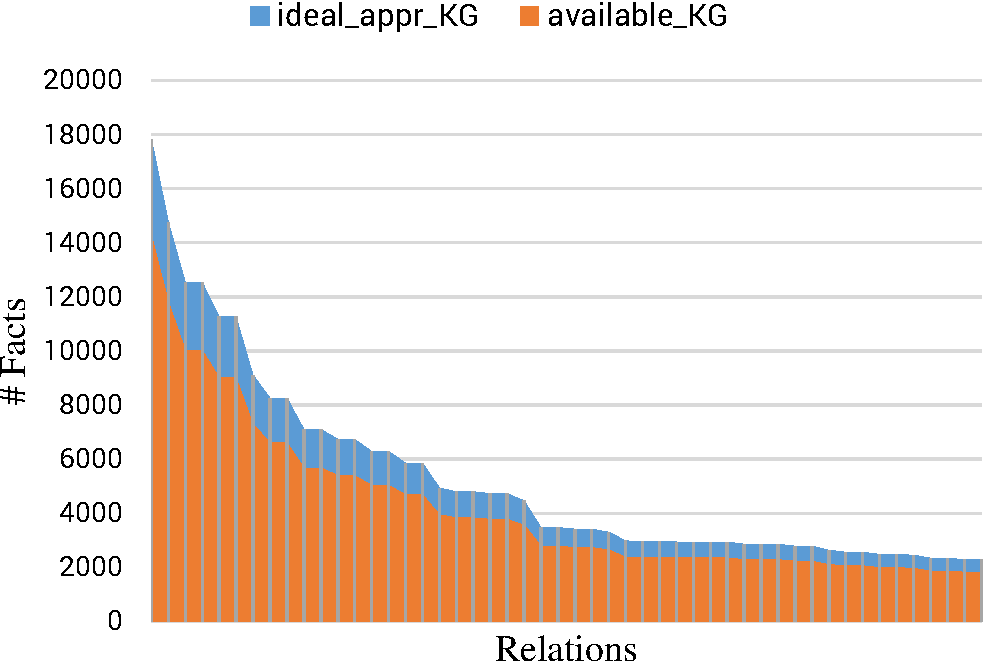
\includegraphics[width=0.5\textwidth]{figures/technical_rp/fb15k_pred_dist-crop.pdf} }}
     \subfloat[Wiki44K]{{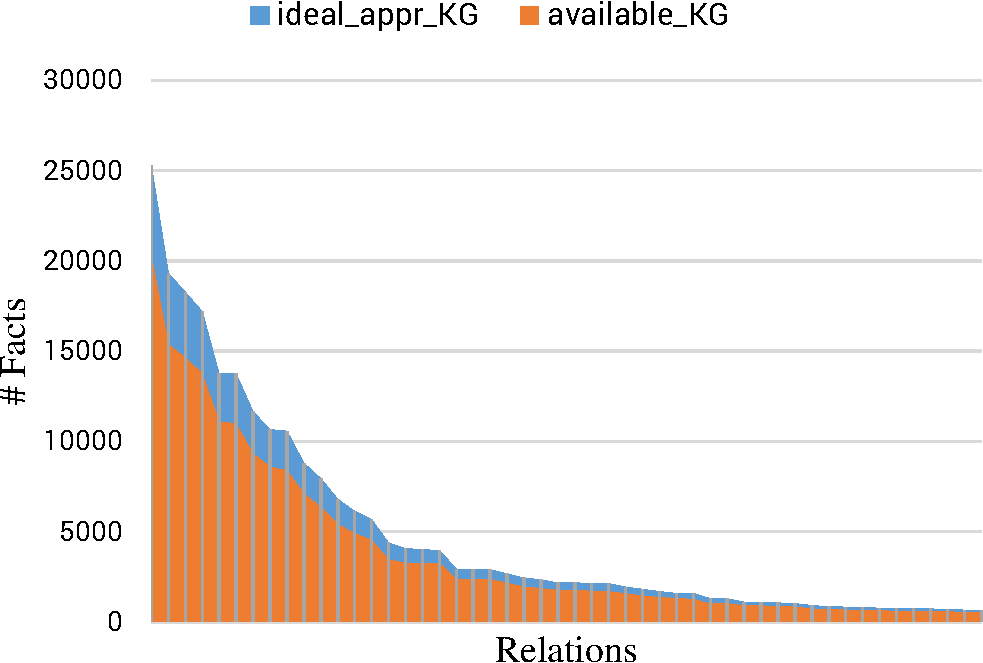
\includegraphics[width=0.5\textwidth]{figures/technical_rp/wiki44k_pred_dist-crop.pdf} }}\\
     \subfloat[IMDB]{{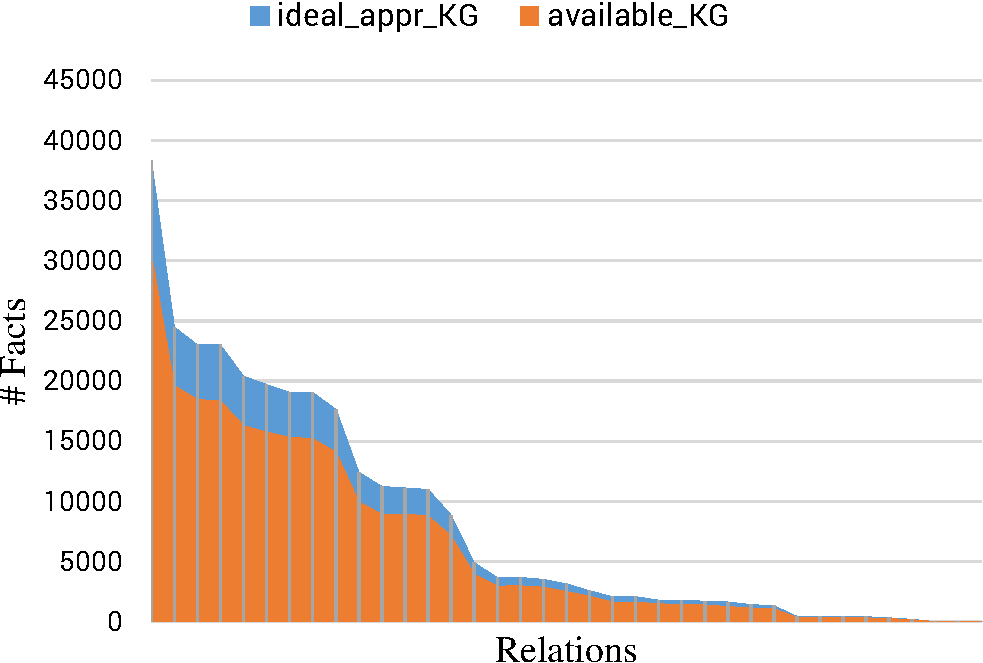
\includegraphics[width=0.5\textwidth]{figures/technical_rp/imdb_pred_dist-crop.pdf} }}
     \caption{Distribution of facts over relations of KGs $\cG^i_{appr}$ and $\cG$.}
     \label{table:pred_distribution}
\end{figure}

\subsection{Embedding Models} 

TransE \cite{Bordes:NIPS2013} and HolE \cite{DBLP:conf/aaai/NickelRP16} are two state-of-the-art embedding models that do not account for external data. In contract, SSP \cite{DBLP:conf/aaai/0005HMZ17} is a state-of-the-art model which accounts for short textual descriptions attached to KG entities. We focus on these 3 embedding models in this work, since they are efficient and relatively simple.
\begin{table}[t]
\centering
\begin{tabular}{|l|r r|r r|r r|r r|r r|r r|} 
 \hline
 DATASET & \multicolumn{4}{|c|}{FB15K} & \multicolumn{4}{|c|}{Wiki44k} & \multicolumn{4}{|c|}{IMDB}\\
 \hline
 MODEL & \multicolumn{2}{|c|}{MRR}& \multicolumn{2}{|c|}{Hits@10(\%)} & \multicolumn{2}{|c|}{MRR}& \multicolumn{2}{|c|}{Hits@10(\%)} & \multicolumn{2}{|c|}{MRR}& \multicolumn{2}{|c|}{Hits@10(\%)} \\
 $Eval.\ setting$ & $Raw$ & $Filt.$ & $Raw$ & $Filt.$ & $Raw$ & $Filt.$ & $Raw$ & $Filt.$ & $Raw$ & $Filt.$ & $Raw$ & $Filt.$\\
 \hline
 TransE& 0.23 & 0.33 & 47.48 & 59.64 & 0.22 & 0.26 & 39.23 & 43.58 & 0.26 & \textbf{0.31} & 36.63 & \textbf{40.39}\\
 HolE & 0.24 & 0.36 & 47.54 & 60.45& 0.14 & 0.18 & 24.54 & 28.38  & 0.21 & 0.26 & 28.27 & 32.08 \\
 SSP & 0.29 & \textbf{0.45}& 55.73 & \textbf{70.35}& 0.26 & \textbf{0.31} & 45.15 & \textbf{51.05} & -- & -- & -- & -- \\
 \hline
\end{tabular}
\caption{Performance of embedding models on the three data sets.}
\label{table:embedding_performance}
\end{table}


We reuse existing implementations of TransE, HolE\footnote{\url{https://github.com/mnick/scikit-kge}}, and SSP\footnote{\url{https://github.com/bookmanhan/Embedding}} and trained these embedding models on the available KGs until convergence using Stochastic Gradient Descent. While we train embedding models on \textit{IMDB} without external text, these embedding models are trained on \textit{FB15K} and \textit{Wiki44K} with 2 different settings: with and without the external textual data. In particular, each entity of \textit{FB15K} and \textit{Wiki44K} links to a small piece of description text, which is extracted from the corresponding Wikidata page. Furthermore, we discard all entities having empty description text for both experimental settings.

For evaluation protocol of the embedding models, we followed the same method of HolE \cite{DBLP:conf/aaai/NickelRP16}. To validate and test the models, we sampled 2000 facts from $\cG^i_{appr} \setminus \cG$ into the validation set, and other 2000 facts into the test set. We report the Mean Reciprocal Rank and the percentage of Hit@10 in Table \ref{table:embedding_performance}. The optimal hyperparameters  of each model and dataset are computed via grid search. We select the hyperparameters, which result in the highest MRR score with \textit{filtered} setting on the validation set. We refer to \cite{DBLP:conf/aaai/NickelRP16} for details.

According to Table \ref{table:embedding_performance}, we compared the effectiveness of the models and selected for each KG the best one. Apart from SSP, which showed the best performance on both FB15K and Wiki44K, we also selected HolE for FB15K and TransE for Wiki44K and IMDB. Note that in this work as a proof of concept we considered some of the most popular embedding models, but conceptually any model (see \cite{DBLP:journals/tkde/WangMWG17} for overview) can be used in our system.

\subsection{Evaluation Metrics} 
To evaluate the learned rules we use the quality of predictions that they produce %through applying the 
when applied on $\cG$, i.e., the more correct facts beyond $\cG$ a ruleset produces, the better it is.  
We consider two evaluation settings: \emph{closed world} setting (CW) and \emph{open world} setting (OW). 
In the CW setting, we define the prediction precision of a rule $r$ and a set of rules $R$ as:
\begin{align*}
  pred\_prec_{CW}(r) = \frac{|\cG_r \cap \cG^i_{appr} \setminus \cG|}{|\cG_r \setminus \cG|},
  \quad 
  pred\_prec_{CW}(R) = \frac{\sum\limits_{r\in R} pred\_prec_{CW}(r)}{|R|}
\end{align*}  
In the OW setting, we also take into account the incompleteness of $\cG^i_{\mi{appr}}$ and  
consider the quality of predictions outside it by performing a random sampling and manually annotating the sampled facts relying on Web resources such as Wikipedia. Thus, we define the OW prediction precision $\mi{pred\_prec_{OW}}$ for a set of rules $R$ as follows:
\[
pred\_prec_{OW}(R) = \frac{|\cG'\cap \cG^i_{\mi{appr}}|+|\cG'\backslash \cG^i_{\mi{appr}}|\times \mi{accuracy(\cG'\backslash \cG^i_{\mi{appr}})}}{|\cG'|}
\]
where $\cG'=\bigcup_{r\in R}\cG_r\backslash \cG$ is the union of predictions generated by rules in $R$, and $\mi{accuracy(S)}$ is the approximated ratio of true facts inside $S$ computed via manual checking of facts sampled from $S$. 
Finally, to evaluate the meaningfulness of exceptions in a rule (i.e., negated atoms) we compute the \textit{revision precision}, which according to~\cite{trantowards} is defined as the ratio of incorrect facts in the difference between predictions produced by the Horn part of a rule and its non-monotonic version over the total number of predictions in this difference (the higher the revision precision, the better the rule exceptions) computed per ruleset. Formally,
\begin{align*}
rev\_prec_{OW}(R) = 1-\frac{|\cG'' \cap \cG^i_{\mi{appr}}|+|\cG''\backslash \cG^i_{\mi{appr}}|\times \mi{accuracy(\cG''\backslash \cG^i_{\mi{appr}})}}{|\cG''|}  
\end{align*}
where $\cG''=\cG_H\backslash \cG_R$ and $H$ is the set of Horn parts of rules in $R$. 
Intuitively, $\cG''$ contains facts not predicted by the rules in $R$ but predicted by their Horn versions. 
 
\subsection{RuLES Configuration}
We run RuLES in several configurations where $\mu_1$ is set to either \textit{standard confidence (Conf)} or \textit{PCA confidence (PCA)}. Furthermore, while we require $\mu_1 \in [0,1]$, we also consider $non\text{-}[0,1]$ metrics, which does not hold this condition, to realize $\mu_1$ (e.g. $conviction$). Meanwhile, $\mu_2$ is computed based on either TransE, HolE, or SSP models.
Throughout the experiments, the configurations are named as \textbf{$\mu_1$-$\mu_2$} (e.g. Conf-HolE). 

\section{Embedding-Based Hybrid Quality Function}
\begin{figure}[t]
     \centering
     \subfloat[Conf-HoLE on FB15K]{{\includegraphics[width=0.5\textwidth]{figures/technical_rp/fb15k_hole_conf-crop.pdf} }\label{fig:fb-conf-hole}}
     \subfloat[Conf-SSP on FB15K]{{\includegraphics[width=0.5\textwidth]{figures/technical_rp/fb15k_ssp_conf-crop.pdf}}\label{fig:fb-conf-ssp}}\\
     \subfloat[PCA-HolE on FB15K]{{\includegraphics[width=0.5\textwidth]{figures/technical_rp/fb15k_hole_pca-crop.pdf} }}
     \subfloat[PCA-SSP on FB15K]{{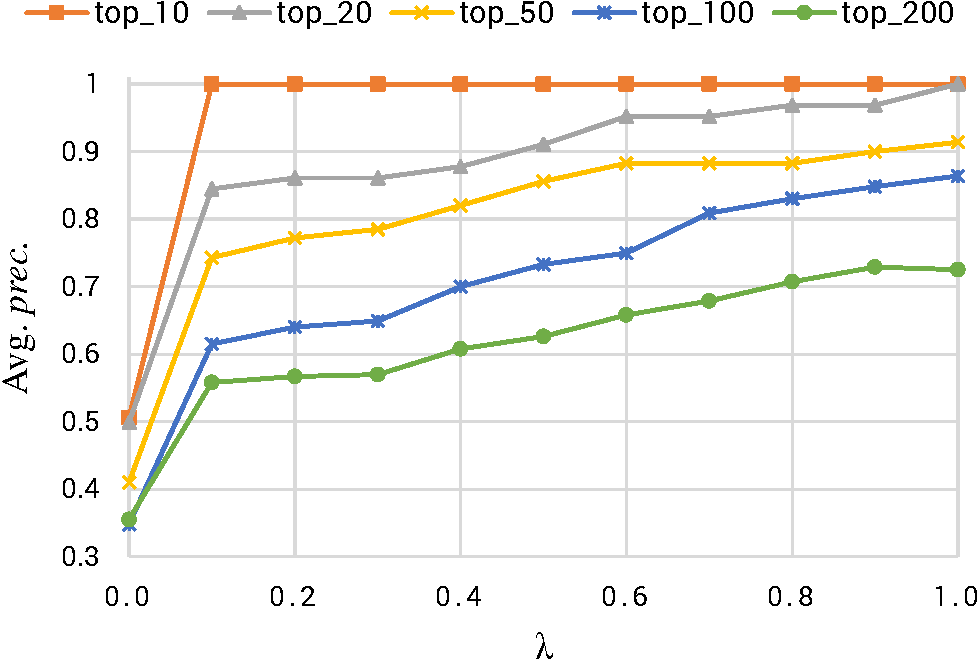
\includegraphics[width=0.5\textwidth]{figures/technical_rp/fb15k_ssp_pca-crop.pdf} }} \\   
     \subfloat[Conv-HolE on FB15K]{{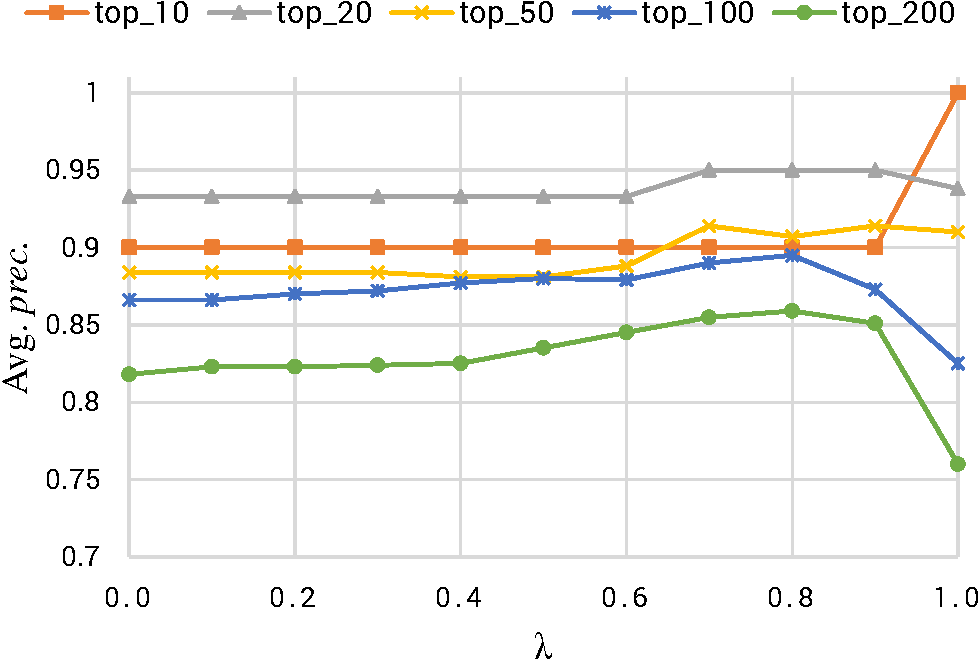
\includegraphics[width=0.5\textwidth]{figures/technical_rp/fb15k_hole_conv-crop.pdf} }}
     \subfloat[Conv-SSP on FB15K]{{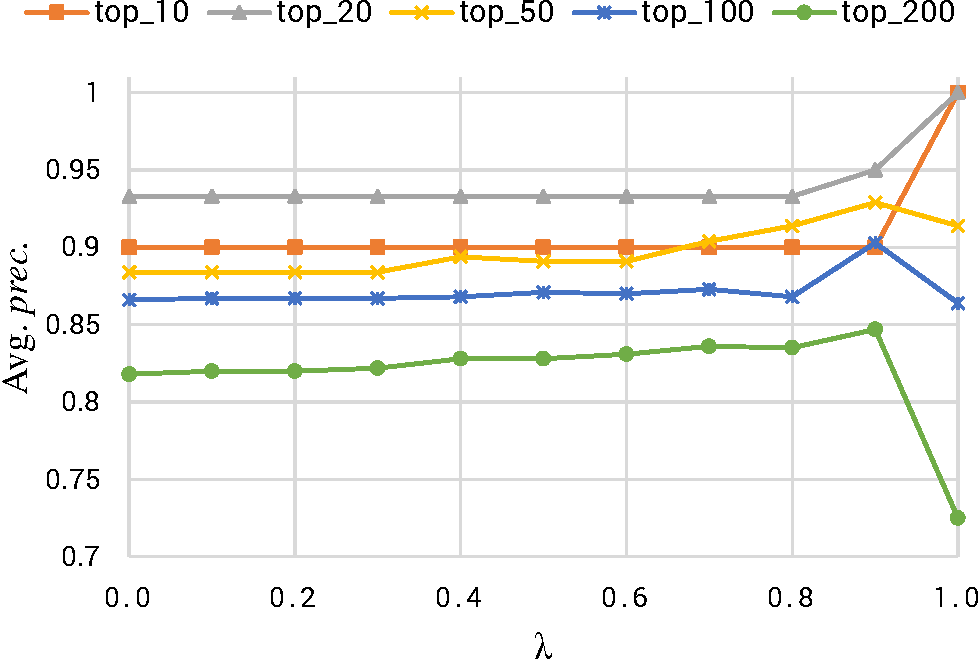
\includegraphics[width=0.5\textwidth]{figures/technical_rp/fb15k_ssp_conv-crop.pdf} }} \\   
     \caption{Avg. prediction precision of the \textit{top-k} rules with various \textit{embedding weights} on FB15K dataset.}
     \label{fig:appendix_exp1_fb15k}
\end{figure} 
\begin{figure}[t]
     \centering
     \subfloat[Conf-TransE on Wiki44K]{{\includegraphics[width=0.5\textwidth]{figures/technical_rp/wiki44k_transe_conf-crop.pdf}}\label{fig:wiki-conf-transe}}
     \subfloat[Conf-SSP on Wiki44K]{{\includegraphics[width=0.5\textwidth]{figures/technical_rp/wiki44k_ssp_conf-crop.pdf}}\label{fig:wiki-conf-ssp}}\\
     \subfloat[PCA-TransE on Wiki44K]{{\includegraphics[width=0.5\textwidth]{figures/technical_rp/wiki44k_transe_pca-crop.pdf} }}
     \subfloat[PCA-SSP on Wiki44K]{{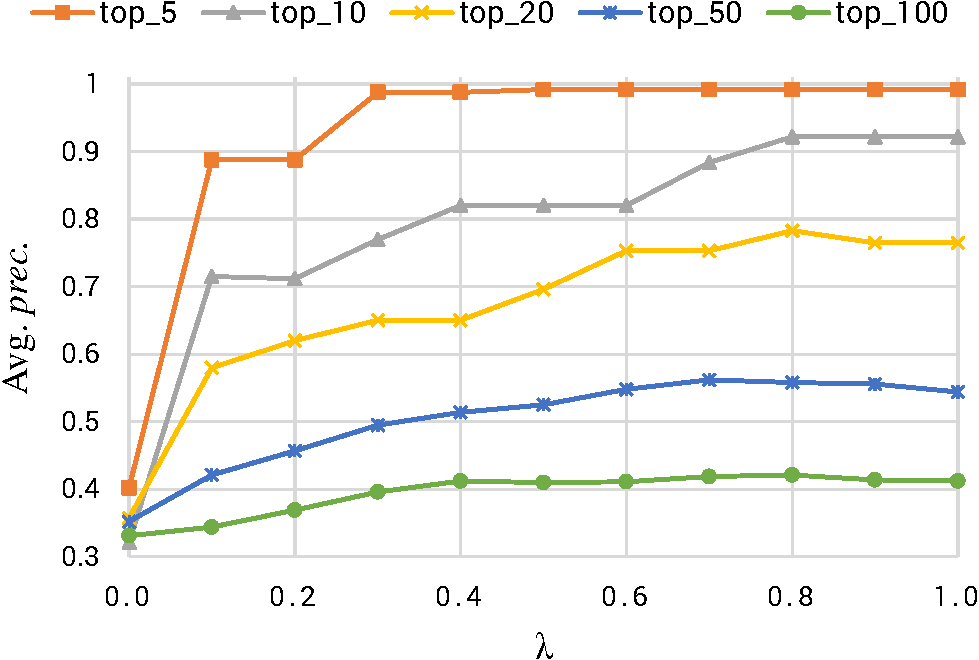
\includegraphics[width=0.5\textwidth]{figures/technical_rp/wiki44k_ssp_pca-crop.pdf} }} \\   
     \subfloat[Conv-TransE on Wiki44K]{{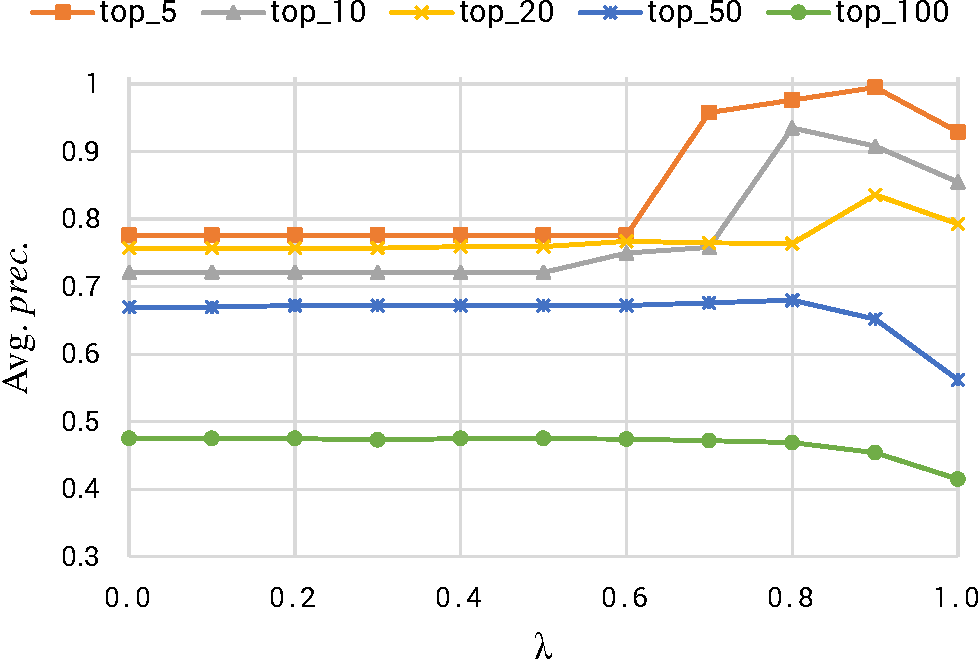
\includegraphics[width=0.5\textwidth]{figures/technical_rp/wiki44k_transe_conv-crop.pdf} }}
     \subfloat[Conv-SSP on Wiki44K]{{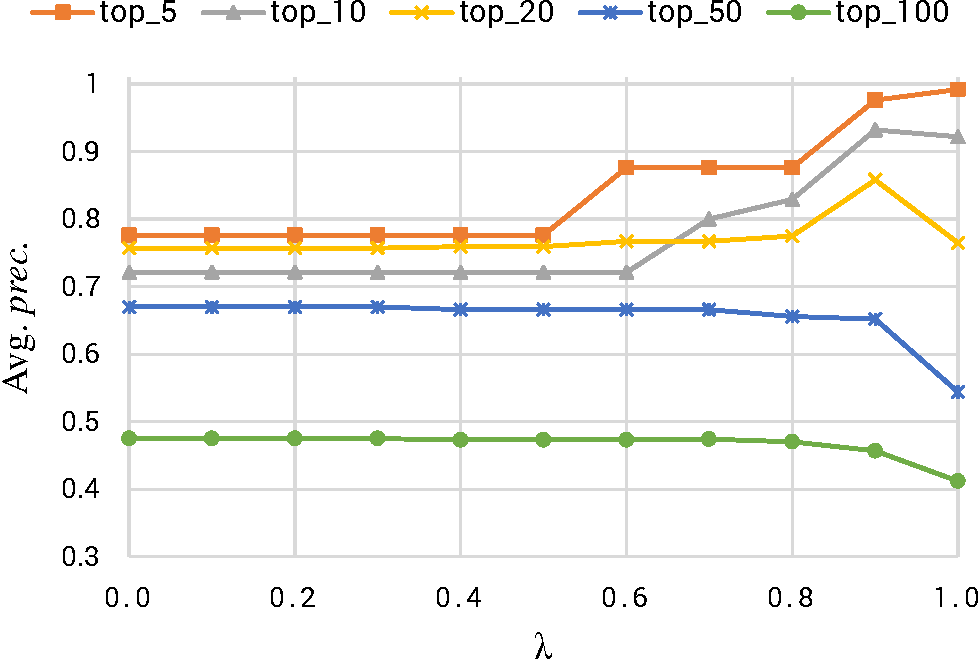
\includegraphics[width=0.5\textwidth]{figures/technical_rp/wiki44k_ssp_conv-crop.pdf} }}\\   
     \caption{Avg. prediction precision of the \textit{top-k} rules with various \textit{embedding weights} on Wiki44K dataset.}
     \label{fig:appendix_exp1_wiki44k}
\end{figure} 

\begin{figure}[t]
     \centering
     \subfloat[Conf-TransE on IMDB]{{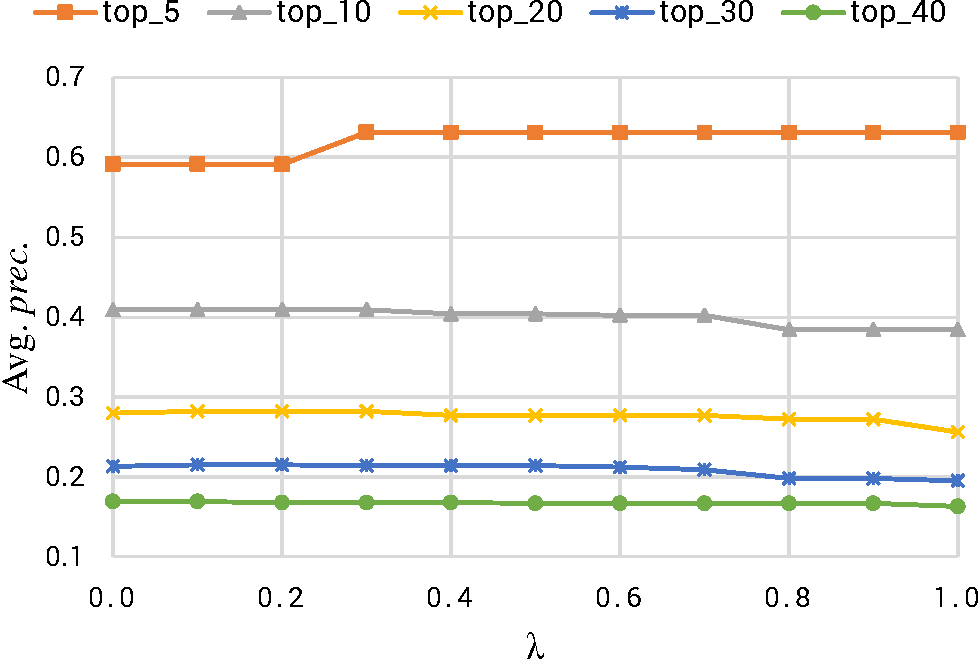
\includegraphics[width=0.5\textwidth]{figures/technical_rp/imdb_transe_conf-crop.pdf} }\label{fig:imdb-conf-transe}}
     \subfloat[PCA-TransE on IMDB]{{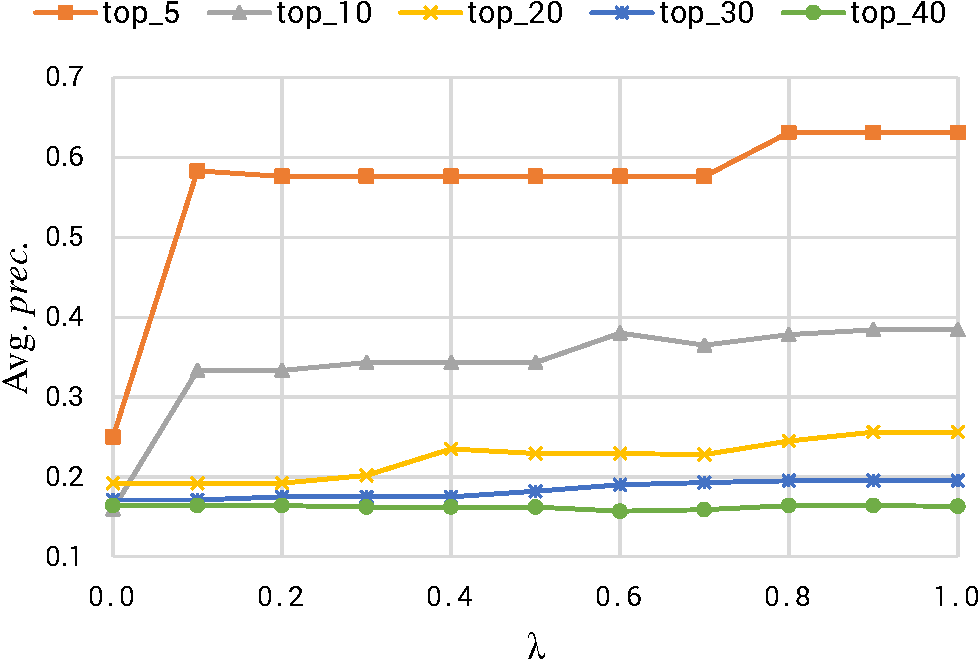
\includegraphics[width=0.5\textwidth]{figures/technical_rp/imdb_transe_pca-crop.pdf} }}\\
     \subfloat[Conv-TransE on IMDB]{{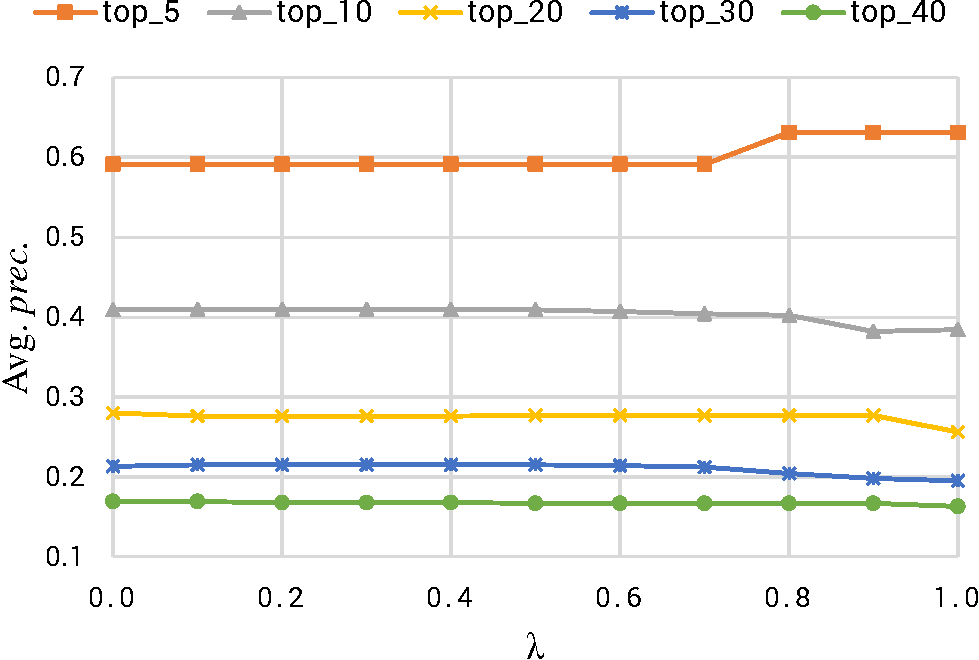
\includegraphics[width=0.5\textwidth]{figures/technical_rp/imdb_transe_conv-crop.pdf} }}     
     \caption{Avg. prediction precision of the \textit{top-k} rules with various \textit{embedding weights} on IMDB dataset.}
     \label{fig:appendix_exp1_imdb}
\end{figure}
\subsection{Hybrid quality function versus standard rule metrics} \label{exp:1}
In this experiment we study the effect of using our hybrid embedding-based 
rule measure $\mu$ from Equation~\ref{eq:hm} on the 
rule ranking compared to traditional measures. 
We do it by first 
learning rules of the form $r:\;h(X,Z) \leftarrow p(X,Y), q(Y,Z)$ from $\cG$ where $\mi{\textit{r-supp}(r,\cG)\geq 10}$, $\mi{conf(r,\cG)\in [0.1,1)}$ and $\mi{\textit{h-cover}(r,\cG)\geq 0.01}$. %at least 
Then, we rank these rules using Equation~\ref{eq:hm} with $\lambda\in \{0, 0.1, 0.2, \dotsc, 1\}$, $\mu_1\in \{\mi{conf,conf_{pca}, conv}\}$ and with $\mu_2$ that is computed by relying on TransE, HolE and SSP.
Note that $\lambda=0$ corresponds to the standard rule measure $\mu_1$ alone.

Figures \ref{fig:appendix_exp1_fb15k}, \ref{fig:appendix_exp1_wiki44k} and \ref{fig:appendix_exp1_imdb} show the %change in the 
average prediction precision $pred\_prec_{CW}$ of the \textit{top-k} rules ranked using our measure $\mu$ for different embedding weights $\lambda$ (\textit{x-axis}). 
In Figures~\ref{fig:fb-conf-hole},~\ref{fig:fb-conf-ssp},~\ref{fig:wiki-conf-transe},~\ref{fig:wiki-conf-ssp} and ~\ref{fig:imdb-conf-transe} %(a,b,d, and e) 
we observe that combining standard confidence ($\mu_1 = conf$)with any %show that combining the confidence with any %other 
%the 
embedding model %results in the increase %rises 
%of 
%in
increases the average prediction precision for %all values of 
%while increasing 
$0\leq \lambda\leq 0.3$. %till it reaches its maximum value around $\lambda=
Moreover, we observe the decrease of prediction precision for $0.4 \leq \lambda\leq 1$ and \textit{top-k} rules learned from FB15K when $k\geq 20$ %starting from \textit{top-20} rules 
and from Wiki44K when $k\geq 10$. %extracted 
%induced from Wiki44K. %\textit{top10}. 
%This behavior is more noticeable . 
This %Hence, it 
shows that the combination of $\mu_1$ and $\mu_2$ gives noticeable positive effect %enhances 
on the prediction results. On the other hand, for $\mu_1=\mi{conf_{pca}}$ the precision increases significantly when combined with embedding models and only decreases slightly %with 
for $\lambda=1$. 
Utilizing $\mi{conf_{pca}}$ instead of $\mi{conf}$ as $\mu_1$ in our hybrid measure is less effective, since 
%The configurations perform worst than standard confidence because 
our training data $\cG$ is randomly sampled %which 
breaking the %local closed world 
partial completeness assumption adopted by the PCA confidence. Meanwhile, with $\mu_1 = conv$, the best value of embedding weight $\lambda$ is close to 1. This is reasonable, since conviction could give us a value greater than 1.

On IMDB dataset, the usage of our hybrid quality measure does improve the quality of result. However, the improvement is not easily noticeable. One explanation is that this dataset is very sparse, which could lead to the ineffectiveness of the embedding models.

\begin{table}[t]
\centering
\begin{tabular}{|c|r r r r r|} 
 \hline
 \multirow{3}{*}{\textbf{\textit{top-k}}} & \multicolumn{5}{|c|}{\textbf{FB15K}}\\
 \cline{2-6}
 & \textbf{{~~~~~}Conf}&  \textbf{{~~~~~}PCA} & \textbf{{~~~~~}Conv} &\textbf{Conf-HolE}& \textbf{Conf-SSP}\\
  & {\scriptsize($\lambda=0$)} & {\scriptsize($\lambda=0$)} & {\scriptsize($\lambda=0$)} & {\scriptsize($\lambda=0.3$)} & {\scriptsize($\lambda=0.3$)}\\
 \hline
\textbf{5} & 0.800 & 0.638 & \textbf{1.000} & \textbf{1.000} & \textbf{1.000}\\
\textbf{10} & 0.900 & 0.506 & 0.900 & \textbf{1.000} & \textbf{1.000}\\
\textbf{20} & 0.900 & 0.499 & 0.933 & 0.950 & \textbf{1.000}\\
\textbf{50} & 0.881 & 0.410 & 0.884 & 0.936 & \textbf{0.937}\\
\textbf{100} & 0.855 & 0.348 & 0.866 & 0.885 & \textbf{0.895}\\
\textbf{200} & 0.842 & 0.355 & 0.818 & 0.870 & \textbf{0.875}\\
 \hline
\end{tabular}
\begin{tabular}{|c|r r r r r|} 
 \hline
 \multirow{3}{*}{\textbf{\textit{top-k}}} & \multicolumn{5}{|c|}{\textbf{Wiki44K}}\\
 \cline{2-6}
 & \textbf{{~~~~~}Conf}&  \textbf{{~~~~~}PCA} & \textbf{{~~~~~}Conv} &\textbf{{~}Conf-Tr.E}& \textbf{Conf-SSP}\\
  & {\scriptsize($\lambda=0$)} & {\scriptsize($\lambda=0$)} & {\scriptsize($\lambda=0$)} & {\scriptsize($\lambda=0.3$)} & {\scriptsize($\lambda=0.3$)}\\
 \hline
 \textbf{5} & 0.800 & 0.402 & 0.776 & \textbf{0.995} & 0.968 \\
\textbf{10} & 0.638 & 0.321 & 0.721 & 0.863 & \textbf{0.932} \\
\textbf{20} & 0.712 & 0.357 & 0.757 & 0.802 & \textbf{0.825} \\
\textbf{50} & 0.670 & 0.352 & 0.670 & \textbf{0.675} & 0.674 \\
\textbf{100} & \textbf{0.477} & 0.331 & 0.475 & 0.474 & 0.474\\
 \hline
\end{tabular}
\begin{tabular}{|c|r r r r|} 
 \hline
 \multirow{3}{*}{\textbf{\textit{top-k}}} & \multicolumn{4}{|c|}{\textbf{IMDB}}\\
 \cline{2-5}
 & \textbf{{~~~~~}Conf}&  \textbf{{~~~~~}PCA} & \textbf{{~~~~~}Conv} &\textbf{{~}Conf-Tr.E}\\
  & {\scriptsize($\lambda=0$)} & {\scriptsize($\lambda=0$)} & {\scriptsize($\lambda=0$)} & {\scriptsize($\lambda=0.3$)}\\
 \hline
\textbf{5} & 0.591 & 0.250 & 0.591 & \textbf{0.631} \\
\textbf{10} & \textbf{0.409} & 0.160 & \textbf{0.409} & \textbf{0.409} \\
\textbf{20} & 0.280 & 0.192 & 0.280 & \textbf{0.282} \\
\textbf{30} & 0.213 & 0.171 & 0.213 & \textbf{0.214} \\
\textbf{40} & \textbf{0.169} & 0.164 & \textbf{0.169} & 0.168 \\
 \hline
\end{tabular}
\caption{Avg. prediction precision of the rules learned using different measures.}
\label{table:avg_quality}
\end{table}


Table~\ref{table:avg_quality} compactly summarizes the average prediction precision of \textit{top-k} rules ranked by
the standard rule measures and our $\mu$ for the best value of $\lambda=0.3$ and highlights the effect of using the better embedding model (text-enhanced vs standard).
%The last two columns for every KG report the results of using $\mu_2$ based on a more advanced embedding model. 
On \textit{FB15K} and \textit{Wiki44K}, we observe that the accuracy of a utilized embedding model is naturally propagated to the accuracy of the rules that we obtain using our hybrid ranking measure $\mu$. This demonstrates that the use of a better embedding model positively effects %should lead to 
the quality of learned rules. 

\subsection{Handling rules with low support}
\begin{figure}[t]
     \centering
     \subfloat[FB15K]{{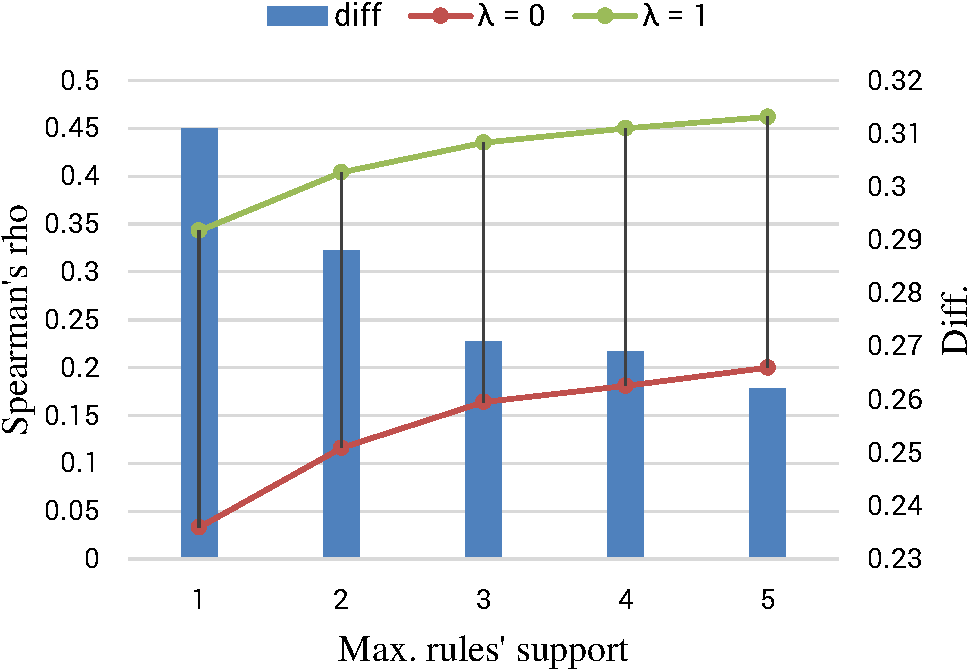
\includegraphics[width=0.5\textwidth]{figures/technical_rp/low_sp_fb15k-crop.pdf} }}
     \subfloat[Wiki44K]{{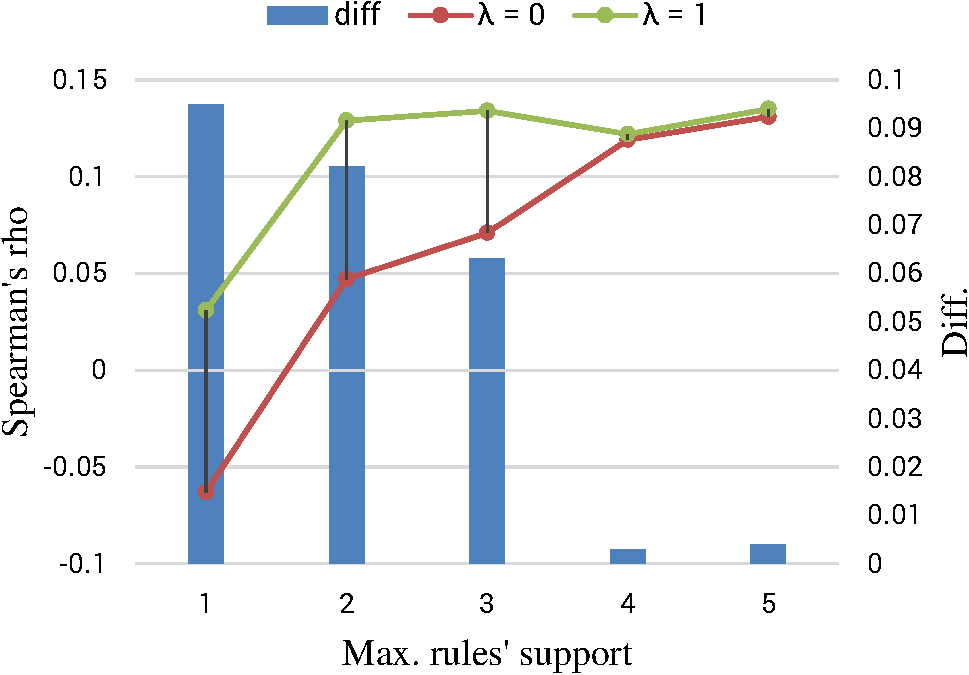
\includegraphics[width=0.5\textwidth]{figures/technical_rp/low_sp_wiki44k-crop.pdf} }}\\
     \subfloat[IMDB]{{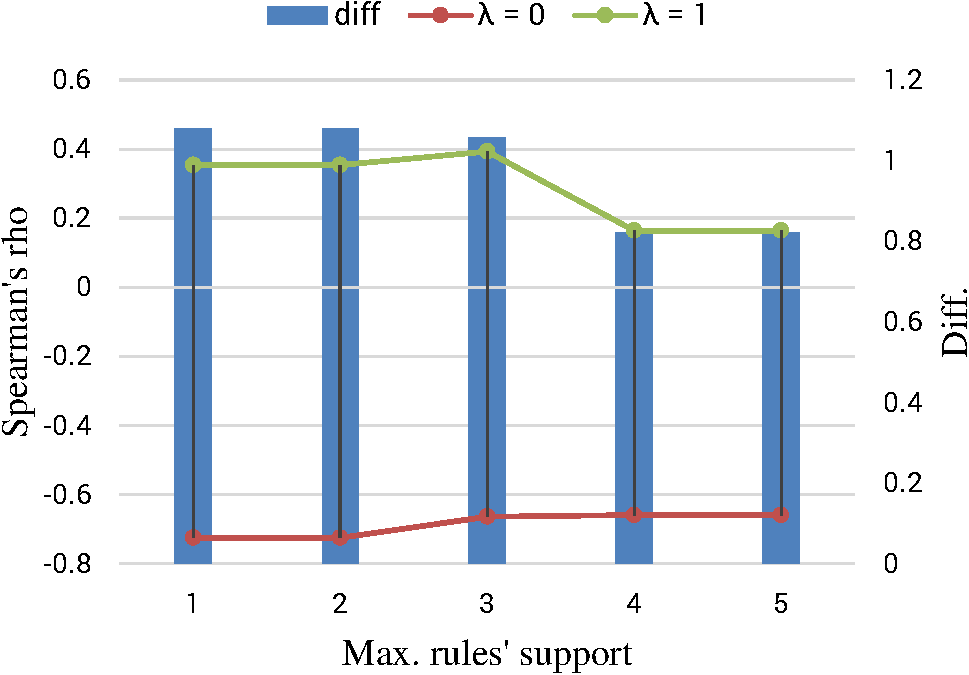
\includegraphics[width=0.5\textwidth]{figures/technical_rp/low_sp_imdb-crop.pdf} }}
     \caption{Spearman's rho of top rules ranked by confidence and the hybrid quality function, with limit on rules' support.}
     \label{fig:low_sp}
\end{figure}
Our hybrid quality function is especially beneficial for assessing rules with low support. Indeed, standard confidence is unreliable for such rules, as it estimates rules' quality by relying only on a small number of rules' instantiations. For example, ignoring all rules having confidence 1 since they do not infer any new facts, when a rule has support 1, its confidence is never greater than 0.5, even though the predicted facts may be true. 

Hybrid quality function $\mu$ fixes this issues by directly looking at the quality of predicted facts, which is achieved by feedback from the embedding models. We verify this hypothesis on \textit{FB15K}, \textit{Wiki44K} and \textit{IMDB} datasets. We also extract rules of form the $r:\;h(X,Z) \leftarrow p(X,Y), q(Y,Z)$ from $\cG$, with $conf(r,\cG) \geq 0.1$ and $\textit{r-supp}(r,\cG) \leq k$, where $k$ indicates the maximum support of rules to be extracted, we try different values of $k \in \{1,2,3,4,5\}$. These rules are then ranked using standard confidence and our hybrid quality function $\mu$. In addition, since we hypothesize that the confidence does not give strong information about the rules in this case, we use $\mu = \mu_2 (\lambda = 1)$, where the hybrid quality function relies only on feedback from the embedding models. To compute $\mu_2$, we use the best embedding models for each dataset: SSP for \textit{FB15K}, \textit{Wiki44K} and TransE for \textit{IMDB}.

To evaluate the quality of the 2 ranked rule lists, we measure the Spearman's rank correlation coefficient (\textit{Spearman's rho}, i.e. Pearson correlation applied to rank)  of rules' confidence or hybrid quality with their $pred\_prec_{CW}$. Figure \ref{fig:low_sp} shows the Spearman's rho of the 2 ranked lists and the difference between them with different values of rules' support limit $k$. The hybrid quality function outperforms standard confidence on 3 datasets, and the results are more visible for lower-support rules.
\section{Horn Rule Learning}
\label{sec:RuLES_vs_AMIE}
%RuLES verses state-of-art}

In this experiment, we compare the Conf-SSP configuration of RuLES (with embedding weight $\lambda = 0.3$) against the state-of-art Horn rule learning system AMIE. We used the default AMIE-PCA configuration with $\mi{conf_{pca}}$ and %  %Also, given the broken partial completeness $\mi{conf_{pca}}$ requires as shown previously, 
% Moreover, we also used the configuration with \textit{standard confidence}, which we refer to as
AMIE-Conf with $\mi{conf}$ measures respectively. For a fair comparison, we set the two configurations of AMIE and our system  to generate rules with at most three positive atoms in the body and  filtered them based on minimum confidence of $0.1$, head coverage of $0.01$ and rule support of $10$ in case of FB15K and $2$ in case of Wiki44K. We then filtered out all rules with $\mi{conf(r,\cG) = 1}$, as they %cannot not infer any new facts. %For evaluation, we use the OW \textit{prediction precision} $pred\_prec_{OW}(R)$ with a sample of 20 prediction outside $\cG^i_{appr}$.
do not produce any predictions.

\setlength{\tabcolsep}{0.1em}
\begin{table}[t]
\centering
\begin{tabular}{|c|r r|r r|r r|r r|r r|r r|}
 \hline
 \multirow{3}{*}{\textbf{\textit{top-k}}}&\multicolumn{6}{|c|}{\textbf{FB15K}} & \multicolumn{6}{|c|}{\textbf{Wiki44K}}\\
 \cline{2-13}&\multicolumn{2}{|c|}{\textbf{AMIE-PCA}}&\multicolumn{2}{|c|}{\textbf{AMIE-Conf}}&\multicolumn{2}{|c|}{\textbf{RuLES}}&\multicolumn{2}{|c|}{\textbf{AMIE-PCA}}&\multicolumn{2}{|c|}{\textbf{AMIE-Conf}}&\multicolumn{2}{|c|}{\textbf{RuLES}} \\
 & \textit{Facts} & \textit{Prec.} & \textit{Facts} & \textit{Prec.} & \textit{Facts} & \textit{Prec.} &\textit{Facts} & \textit{Prec.} &\textit{Facts} & \textit{Prec.} &\textit{Facts} & \textit{Prec.} \\
 \hline
 \textbf{20} & 1029 & 0.28 & 82 & 0.63 & 44 & 1.00 & 185 & 0.73 & 91 & 0.95 & 3291 & 0.98\\
 \textbf{50} & 1716 & 0.43 & 190 & 0.74 & 186 & 0.92 & 47099 & 0.10 & 3594 & 0.95 & 6154 & 0.88 \\
\textbf{100} & 3085 & 0.65 & 255 & 0.78 & 539 & 0.80 & 56831 & 0.20 & 13870 & 0.83 & 13253 & 0.82 \\
\textbf{200} & 10586 & 0.62 & 1210 & 0.83 & 1205 & 0.88 & 82288 & 0.39 & 19538 & 0.72 & 20408 & 0.73 \\
\textbf{500} & 40050 & 0.51 & 2702 & 0.75 & 7124 & 0.95 & 219264 & 0.35 & 124836 & 0.23 & 128256 & 0.48 \\
 \hline
\end{tabular}
\caption{Prediction precision of the \textit{top-k} rules generated by RuLES and AMIE.}
\label{table:amie_vs_RuLES}
\end{table}
\setlength{\tabcolsep}{0.2em}


\begin{table}[t]
\centering
\begin{tabular}{|c|r r|r r|}
 \hline
 \multirow{3}{*}{\textbf{\textit{top-k}}}&\multicolumn{4}{|c|}{\textbf{Family}}\\
 \cline{2-5}&\multicolumn{2}{|c|}{\textbf{NeuralLP}}&\multicolumn{2}{|c|}{\textbf{Conf-TransE}}\\
 & \textit{Facts} & \textit{Prec.} & \textit{Facts} & \textit{Prec.} \\
 \hline
\textbf{10} & 3709 & 0.72 & 4201 & 0.68 \\
\textbf{20} & 8821 & 0.53 & 6957 & 0.72 \\
\textbf{30} & 11337 & 0.49 & 9368 & 0.71 \\
\textbf{40} & 14662 & 0.46 & 11502 & 0.72 \\
\textbf{50} & 18768 & 0.40 & 14547 & 0.62 \\
 \hline
\end{tabular}
\caption{Prediction precision of the \textit{top-k} rules generated by NeuralLP and RuLES.}
\label{table:neurallp_vs_rules}
%\thi{This is added to compare NeuralLP and RuLES}
\end{table}


Table~\ref{table:amie_vs_RuLES} shows the number of facts (see the \textit{Facts} column) predicted by %for 
the set $R$ of \textit{top-k} rules %generated 
in the described settings %. For each set of predictions produced by the set  $R$ of \textit{top-k} rules 
and their prediction precision $pred\_prec_{OW}(R)$ (see the \textit{Prec.} column). %shows the %OW \textit{prediction precision} 
The size of the random sample 
% computed based on facts 
outside $\cG^i_{appr}$ is 20. % and a sample of 20 predictions outside $\cG^i_{appr}$. 
We can observe that on FB15K, RuLES consistently outperforms both AMIE configurations. The \textit{top-20} rules have the highest precision difference (outperforming AMIE-PCA and AMIE-Conf by $72\%$ and $37\%$ respectively).
% AMIE and AMIE-Conf. 
This is explained by the fact that the hybrid embedding quality penalizes rules with higher number of false predictions. %Also 
%Moreover, f
For Wiki44K, RuLES is capable of achieving better precision in most of the cases. %Moreover, for %in 
Notably, for the \textit{top-20} rules RuLES predicted significantly more facts then competitors yet with a high precision. 

In table~\ref{table:neurallp_vs_rules}, we compare RuLES with the recently developed NeuralLP system~\cite{DBLP:conf/nips/YangYC17}. For this we used the Family dataset offered by the authors\footnote{\url{https://github.com/fanyangxyz/Neural-LP}} %with their software %their system which contains 28K facts %distributed covering 
with 28K facts over 3K entities and 12 relations. %As observed 
Starting from the \textit{top-20} rules RuLES is capable of achieving significantly better precision. For the \textit{top-10} rules the precision of NeuralLP is slightly better, but RuLES predicts many more facts.

%!TEX root = ../main.tex


\begin{table}[t]
\centering
\small
\begin{tabular}{|cl|}
	\hline
	%$r_1:$ & $has\_family(X, Y) \leftarrow has\_child(Z, X), has\_family(Z, Y), \textbf{not}\ has\_mother(X, Z).$\\
$r^1{:}$ & $\mi{nationality(X{,}\, Y)}\, {\leftarrow}\, \mi{graduated\_from(X{,}\, Z)}{,}\, \mi{in\_country(Z{,}\, Y)},
	\textbf{not}\ \mi{research\_uni(Z)}$\\
$r^2{:}$ & $\mi{scriptwriter\_of}(X{,}\, Y)\, {\leftarrow}\, \mi{preceded\_by(X{,}\, Z)}{,}\, \mi{scriptwriter\_of(Z{,}\, Y)},
\textbf{not}\ \mi{tv\_series(Z)}$\\
$r^3{:}$ &$\mi{noble\_family(X{,}\, Y)}\, {\leftarrow}\, \mi{ spouse(X{,}\, Z)}{,}\, \mi{noble\_family(Z{,}\, Y)}{,}\,  \textbf{not}\ \mi{ chinese\_dynasties(Y)}$\\
%$r_3:$ &$\mi{sister(X, Y)} \leftarrow \mi{sister(Y, X)}, \textbf{not}\ \mi{brother(X, Y)}$\\

	\hline
\end{tabular}
\caption{Example rules with exception generated by RuLES.}
\vspace*{-3mm}
\label{figure:examples}
\end{table}


\section{RuLES for Exception-Aware Rule Learning}
%----------------------------------------------------------------%
In this experiment, we aim at evaluating the effectiveness of RuLES %in
for learning exception-aware rules.
First, consider in Table~\ref{figure:examples} examples of such rules learned by RuLES over Wiki44K dataset. 
%While %the rule $r_1$ states that a child has the family name from the paternal side and not from the maternal side, the 
 The first rule $r^1$ says that a person is a citizen of the country where his alma mater is located, unless it is a research institution, %university, 
since most %of 
researchers in universities are foreigners. The second rule $r^2$ states that the scriptwriter of some artistic work is also the scriptwriter of its sequel unless it is a TV series, which actually reflects the common practice of having several screenwriters for different seasons. Additionally, $r^3$ encodes that someone belonged to a %royal 
noble family if his/her %the 
spouse is also from the same noble family, excluding the Chinese dynasties. % noble families.

 %Additionally, $r_3$ captures the common sense rule that for two individuals $x,y$ if $y$ is the sister of $x$, then $x$ should also be sister of $y$ unless $x$ is actually the brother of $y$.

%Besides RuLES we also used in the evaluation 
To quantify the quality of RuLES in learning non-monotonic rules, we compare the Conf-SSP configuration of RuLES (with embedding weight $\lambda = 0.3$) with RUMIS~\cite{trantowards}, which is a non-monotonic rule revision system which finds exceptions by minimizing the conflicts between the induced rules. RUMIS learns rules %in 
of the form %of 
$\mi{r:\;h(X,Z) \leftarrow p(X,Y), q(Y,Z), not\; E}$, where $E$ is either $e(X,Z)$ or $\textit{type}(X,t)$ %(\eg type relation); 
%where 
with $t\in \cC_\cG$.
%thus, f
For a fair comparison we restricted RuLES to learn rules of the same form. %of rules.  
We configured both systems %to learn rules 
%with 
setting the minimum rule support threshold to %$\textit{r-supp}(r,\cG)\geqslant 
$10$ and exception confidence for RuLES to $0.05$. %Also 
%Moreover, %for RuLES, 
%we discard rules having exception confidence $\textit{e-conf}(r,\cG)\leqslant 0.05$. 
To enable the systems to %mine %ing 
learn rules with exceptions of the form %following 
$\textit{type}(X,t)$, we enriched the KGs with \textit{type} information from the original Freebase and Wikidata graphs. %Nevertheless, 
%However, types were only considered in the negated part of the body. % while adding exception atoms. 
%Finally, %we keep 
%rules with more than one negated atom were dropped. %a single negative atom. 


% \begin{table}[t]
% \centering
% \begin{tabular}{|r|r r|r r|r r|r r|}
%  \hline
%  \multirow{3}{*}{$top-k$}&\multicolumn{4}{|c|}{FB15K} & \multicolumn{4}{|c|}{WIKI44K}\\
%  \cline{2-9}&\multicolumn{2}{|c|}{RUMIS}&\multicolumn{2}{|c|}{RuLES}&\multicolumn{2}{|c|}{RUMIS}&\multicolumn{2}{|c|}{RuLES} \\
%  & $Avg.scr.$ & $Avg.inc.$ & $Avg.scr.$ & $Avg.inc.$& $Avg.scr.$ & $Avg.inc.$& $Avg.scr.$ & $Avg.inc.$ \\
%  \hline
%  20 & 0.791 & 0.024 & 1.000 & 0.047 & 0.743 & 0.067 & 0.803 & 0.024 \\
%  50 & 0.826 & 0.015 & 1.000 & 0.045 & 0.609 & 0.054 & 0.701 & 0.026 \\
% 100 & 0.859 & 0.026 & 0.990 & 0.047 & 0.417 & 0.033 & 0.539 & 0.011 \\
% 200 & 0.848 & 0.034 & 0.977 & 0.065 & 0.253 & 0.022 & 0.339 & 0.017 \\
% 500 & 0.745 & 0.043 & 0.958 & 0.079 & -- & -- & -- & -- \\
% \hline
% \end{tabular}
% \caption{Average prediction score of some top non-monotonic rules from RuLES vs RUMIS.}
% \label{table:exception_prediction_result}
% \vspace*{-3mm}
% \end{table}
\begin{table}[t]
\centering
\begin{tabular}{|c|r r|r r|r r|r r|}
 \hline
 \multirow{3}{*}{\textbf{\textit{top-k}}}&\multicolumn{4}{|c|}{\textbf{FB15K}} & \multicolumn{4}{|c|}{\textbf{Wiki44K}}\\
 \cline{2-9}&\multicolumn{2}{|c|}{\textbf{RUMIS}}&\multicolumn{2}{|c|}{\textbf{RuLES}}&\multicolumn{2}{|c|}{\textbf{RUMIS}}&\multicolumn{2}{|c|}{\textbf{RuLES}} \\
 & $Facts$ & $Prec.$ & $Facts$ & $Prec.$& $Facts$ & $Prec.$& $Facts$ & $Prec.$ \\
 \hline
\textbf{20} & 672 & 0.95 & 34 & 0.97 & 5844 & 0.93 & 5640 & 0.93 \\
\textbf{50} & 1797 & 0.94 & 158 & 0.99 & 8585 & 0.83 & 13333 & 0.84 \\
\textbf{100} & 2672 & 0.94 & 434 & 0.99 & 21081 & 0.76 & 25265 & 0.81 \\
\textbf{200} & 4103 & 0.87 & 1155 & 0.96 & 50957 & 0.51 & 43677 & 0.67 \\
\textbf{500} & 13439 & 0.76 & 5466 & 0.90 & -- & -- & -- & -- \\
\hline
\end{tabular}
\caption{Prediction precision for the \textit{top-k} rules learned by RUMIS and RuLES.}
\label{table:exception_prediction_result}
\end{table}
% \begin{table}[t]
% \centering
% \begin{tabular}{|r|r r|r r|}
%  \hline
%  \multirow{2}{*}{$top-k$}&\multicolumn{2}{|c|}{FB15K} & \multicolumn{2}{|c|}{WIKI44K}\\
%  \cline{2-5} & RUMIS & RuLES & RUMIS & RuLES \\
%  \hline
%  10 & 0.850 & 0.868 & 0.300 & 0.637 \\
%  %20 & 0.675 & 0.871 & 0.175 & 0.514 \\
%  50 & 0.490 & 0.814 & 0.204 & 0.421 \\
% 100 & 0.590 & 0.785 & 0.124 & 0.271 \\
% 200 & 0.608 & 0.762 & -- & -- \\
% \hline
% \end{tabular}
% \caption{Average revision score of some top rules from RuLES vs RUMIS.}
% \label{table:exception_revision_result}
% \end{table}
\begin{table}[t]
\centering
\begin{tabular}{|r|r r|r r|r r|r r|}
 \hline
 \multirow{3}{*}{\textbf{\textit{top-k}}}&\multicolumn{4}{|c|}{\textbf{FB15K}} & \multicolumn{4}{|c|}{\textbf{Wiki44K}}\\
 \cline{2-9}&\multicolumn{2}{|c|}{\textbf{RUMIS}}&\multicolumn{2}{|c|}{\textbf{RuLES}}&\multicolumn{2}{|c|}{\textbf{RUMIS}}&\multicolumn{2}{|c|}{\textbf{RuLES}} \\
 & $Facts$ & $Prec.$ & $Facts$ & $Prec.$& $Facts$ & $Prec.$& $Facts$ & $Prec.$ \\
 \hline
\textbf{20} & 76 & 0.70 & 111 & 0.68 & 63 & 0.47 & 81 & 0.94 \\
\textbf{50} & 126 & 0.51 & 435 & 0.74 & 191 & 0.28 & 611 & 0.69 \\
\textbf{100} & 183 & 0.43 & 680 & 0.76 & 543 & 0.49 & 1698 & 0.79 \\
\textbf{200} & 310 & 0.30 & 1112 & 0.87 & 4861 & 0.40 & 3175 & 0.80 \\
\textbf{500} & 1155 & 0.53 & 3760 & 0.59 & -- & -- & -- & -- \\
\hline
\end{tabular}
%\caption{Precision of erroneous predictions avoided by rules of RUMIS and RuLES }
\caption{Revision precision for the \textit{top-k} rules learned by RUMIS and RuLES.}
\label{table:exception_revision_result}
\end{table}

%For evaluation, We compute $pred\_prec_{OW}(R)$ for \textit{top-k} rules. 

From the list of mined rules from our system, we keep only rules having some exceptions. If there exist more than 1 such rule having the same positive part, we keep only the one with the highest hybrid quality. In addition, to ensure that the added exception is meaningful, from the list of generated rules from both systems, we keep only rules, whose positive part has standard confidence less than 0.8.

Table~\ref{table:exception_prediction_result} reports the number of predictions produced by a rule set $R$ of %for 
\textit{top-k} non-monotonic rules learned %generated 
by both systems as well as %. For each set $R$ of \textit{top-k} rules, we compute 
their precision $pred\_prec_{OW}(R)$ with a sample of 20 prediction outside $\cG^i_{appr}$. The results show that RuLES consistently outperforms RUMIS %for 
on both datasets. For Wiki44K, and $k\in\{50,100\}$, the \textit{top-k} rules produced by RuLES predicted more facts than those induced by the competitor %as many facts as 
%than RUMIS 
achieving %but with 
higher overall precision. 
Regarding the number of predictions, the converse holds for the FB15K KG; however, the rules learned by RuLES are still more accurate.
%However, in FB15K, the rules generated by RuLES predicted less facts as discussed previously in Section~\ref{sec:RuLES_vs_AMIE}. Note that, the lower the rank of the learned rules, the higher the effect of RuLES in enhancing the prediction quality.

To evaluate the quality of the chosen exceptions, we compare the $rev\_prec_{OW}(R)$ with a sample of 20 predictions. %as explained in Section~\ref{sec:exper_setup}. %As illustrated 
Observe that in Table~\ref{table:exception_revision_result}, rules induced by RuLES prevented the generation of more facts than RUMIS. %those of RUMIS. 
In all of the cases apart from \textit{top-20} for FB15K, our system %RuLES 
managed to remove %achieves higher precision in removing 
a larger fraction of erroneous predictions. %than RUMIS. 
For Wiki44K, RuLES consistently performs twice as good as RUMIS. 
In conclusion, the guidance from the embedding model %using our %hybrid embedding-based quality 
exploited in our system %measure $\mu$ 
%allows us to learn %ing 
%better exception-aware rules, since the feedback from the embedding model 
gives us hints on which among the possible exception candidates likely correspond to noise.   

\section{Summary}
Conducted experiments demonstrate a highly positive impact of the integration of an embedding model on the quality of learned rules. By using an good embedding model, our mining algorithm can extract rules with better predictions' quality, and also capture more meaningful exceptions in comparison with standard methods. 

%  In addition, to see how meaningful the added exception are, table \ref{table:exception_revision_result} reports the precision of removed facts adding exception from some $k$ rules of both systems. The precision of correctly removed facts is also computed by first by looking at $\cG^i_{appr} \setminus \cG$ and second by sampling 20 facts and checking manually ($\cG^i \setminus \cG^i_{appr}$). We can easily notice that our system generates more predictive rules on both datasets in comparison with RUMIS. The reason behind is that RuLES is capable of detecting better exceptions.



%In this experiment, we aim at measuring the quality of our system RuLES on mining exceptions by using the hybrid rule quality scoring function. We use RUMIS \cite{}, which is a state-of-the-art non-monotonic rules mining system, as a baseline to compare our system with. While RUMIS finds exceptions based on only the KG itself, our approach may consider exceptions based on external sources through the embeding models. The setting of the experiment is as follows. We run RUMIS on training KG $\cG$ using the default setting and with OPM ranking method, which is considered its best exception ranking method (see \cite{trantowards}). To reduce running time for RUMIS, we allow only rules with support at least 10. While RUMIS mines only non-monotonic rules with fixed form of the positive part with 3 atoms and support at most 1 exception, our system can generate rules having various forms of positive part, and can even theoretically support more than 1 exception. However, to achieve a fair comparison and reduce the search space, we run our system with the similar setting as RUMIS. In particular, we run our system to generate rules having 3 binary positive atoms and/or 1 additional exception atom. With \textit{exception instantiated atom}, we only allow \textit{\textless rdf:type\textgreater} predicate (i.e. unary predicate), which is the same as in RUMIS. We collect these \textit{\textless rdf:type\textgreater} information for FB15K and Wiki44K from the the whole Freebase and Wikidata dumps, correspondingly. We set the exception coverage of our system to 0.05, minimum rule support also to 10. Other settings regarding selected embedding models, embedding weight and additional filters are similar to the previous experiment. 


%%%%%%%%%%%%%%%%%%%%%%%%%%%% Old text


%% OLD TEXT
%\item \textit{Wikidata} This is a free, community-based knowledge base maintained by the Wikimedia Foundation. In our experiments, we created a subset of Wikidata dump from December 2014 by choosing triples that have entities appearing at least 20 times in the whole dataset, and then selecting top 100 predicates that have most number of facts. We end up with a new dataset with 44k entities, 100 predicates and 250K binary facts. We call this Wiki44K.
%
%% \item \textit{IMDB}\footnote{http://www.imdb.com/} We construct a domain-specific KG from IMDB dataset, which is also used in \cite{Tran2017}. The KG consists of 118K entities, 37 binary predicates, 17K unary predicates and 583K facts (in which, 301K are binary facts).
%\item \textit{Freebase} This is a huge knowledge graph consisting of general facts. To meet the requirement of running both rule mining and embedding, we adopt FB15K \cite{Bordes:NIPS2013}, a dataset containing 15K entities, 1345 binary predicates and 592K binary facts.
%We would like to train the embedding models on the 2 datasets with 2 different settings: with and without the external textual data. In particular, each entity of these datasets is linked with a small piece of description text, which is extracted from the corresponding Wikidata page. Furthermore, we discard all entities having empty description text for both experiments' setting.

%Since obtaining a real life complete ideal KG $\cG^i$ for automatic evaluation is hard, these datasets are used as an approximation $\cG^i_{appr}$ of $\cG^i$. For each dataset, we sample 80\% of facts into the training set (i.e. available graph $\cG$). The rest 20\% will be used for other purposes such as validating or testing.
%% In addition, we ensure that this ratio are equal for each unique predicate. As a side effect, each entity will be connected to at least one other entity.




%%% Old text
%TransE \cite{Bordes:NIPS2013} and HolE \cite{DBLP:conf/aaai/NickelRP16} are two state-of-the-art embedding models regarding the setting of no external data. Meanwhile, when talking about embedding models using additional texts, SSP \cite{DBLP:conf/aaai/0005HMZ17} plays an important part. Apart from prediction quality, these models also have a good running time and memory complexity. Hence, we choose them to evaluate our approach. We reuse the implementation of TransE, HolE from \footnote{https://github.com/mnick/scikit-kge}, and SSP from \footnote{https://github.com/bookmanhan/Embedding}.
%
%We train these embedding models on the available KG $\cG$ of the two datasets Wiki44K and FB15K until convergence using Stochastic Gradient Descent. For evaluation protocol of the embedding models, we use the same method as in TransE \cite{Bordes:NIPS2013} and HolE \cite{DBLP:conf/aaai/NickelRP16}. To validate and test the models, we sampled 2000 facts from the rest 20\% of the dataset (i.e. $\cG^i_{appr} \setminus \cG$) into the validation set, and other 2000 facts into the test set. We report the Mean Reciprocal Rank and the percentage of Hit@10 in table \ref{table:embedding_performance}. The optimal hyperparameters  of each model and dataset are figured out by doing grid search. We select the hyperparameters, which result in the highest MRR score with filtered setting on the validation set. To get a better understanding about how the evaluation is performed, see \cite{Bordes:NIPS2013}.

%\begin{table}[t]
\centering
\begin{tabular}{|l|r r|r r|r r|r r|r r|r r|} 
 \hline
 DATASET & \multicolumn{4}{|c|}{FB15K} & \multicolumn{4}{|c|}{Wiki44k} & \multicolumn{4}{|c|}{IMDB}\\
 \hline
 MODEL & \multicolumn{2}{|c|}{MRR}& \multicolumn{2}{|c|}{Hits@10(\%)} & \multicolumn{2}{|c|}{MRR}& \multicolumn{2}{|c|}{Hits@10(\%)} & \multicolumn{2}{|c|}{MRR}& \multicolumn{2}{|c|}{Hits@10(\%)} \\
 $Eval.\ setting$ & $Raw$ & $Filt.$ & $Raw$ & $Filt.$ & $Raw$ & $Filt.$ & $Raw$ & $Filt.$ & $Raw$ & $Filt.$ & $Raw$ & $Filt.$\\
 \hline
 TransE& 0.23 & 0.33 & 47.48 & 59.64 & 0.22 & 0.26 & 39.23 & 43.58 & 0.26 & \textbf{0.31} & 36.63 & \textbf{40.39}\\
 HolE & 0.24 & 0.36 & 47.54 & 60.45& 0.14 & 0.18 & 24.54 & 28.38  & 0.21 & 0.26 & 28.27 & 32.08 \\
 SSP & 0.29 & \textbf{0.45}& 55.73 & \textbf{70.35}& 0.26 & \textbf{0.31} & 45.15 & \textbf{51.05} & -- & -- & -- & -- \\
 \hline
\end{tabular}
\caption{Performance of embedding models on the three data sets.}
\label{table:embedding_performance}
\end{table}




%First, we focus on comparing our hybrid rule quality scoring function with the two standard rule assessing methods: standard confidence (used by WarmeR) and PCA confidence (used by AMIE). To achieve fair comparison, we only aim at assessing rules having the following form:
%\begin{align*}
%r(X,Z) \leftarrow p(X,Y), q(Y,Z)
%\end{align*}
%Experiment is conducted on both Wiki44K and FB15K datasets. We extract rules of the above form from the training KG $\cG$ that have support at least 10, standard confidence at least 0.1 and head coverage 0.01. All rules with standard confidence 1.0 are also removed, since they do not predict any new facts. These rules are then ordered based on different rule ranking metrics: standard confidence, PCA confidence and our hybrid quality. We computed different versions of hybrid quality, where we use different embedding weights, with standard confidence and PCA confidence as the rule-based metric part. With the setting of no description texts, according to table \ref{table:embedding_performance}, we use TransE for the Wiki44K dataset and HolE for the FB15K dataset, which are the corresponding better models. In addition, we also use SSP model for both datasets. The assessment of these ranking methods are then performed by comparing predictions of these rules on the training set $\cG$ with the approximation $\cG^i_{appr}$. In particular, following \cite{DBLP:conf/semweb/TanonSRMW17}, each rule is given a prediction score, which is computed as the number of predictions inside $\cG^i_{appr} \setminus \cG$ over the number of predictions outside $\cG$:
%\begin{align*}
%    prediction\_score(r) = \frac{|\cG_r \cap \cG^i_{appr} \setminus \cG|}{|\cG_r \setminus \cG_a|}
%\end{align*}
%\captionsetup[subfigure]{textfont=scriptsize}
% \begin{figure}[t]
%    \centering
%    % Gad: to unify legend and save space
%    \subfloat{{\includegraphics[width=0.5\textwidth]{figures/legend.pdf} }}\\[-2ex]
%    \setcounter{subfigure}{0}%
%    \subfloat[Confidence + HolE]{{\includegraphics[width=0.5\textwidth]{figures/fb15k_hole_conf-crop.pdf} }}
%    \subfloat[Confidence + SSP]{{\includegraphics[width=0.5\textwidth]{figures/fb15k_ssp_conf-crop.pdf} }}\\
%    \subfloat[PCA Confidence + HolE]{{\includegraphics[width=0.5\textwidth]{figures/fb15k_hole_pca-crop.pdf} }}
%    \subfloat[PCA Confidence + SSP]{{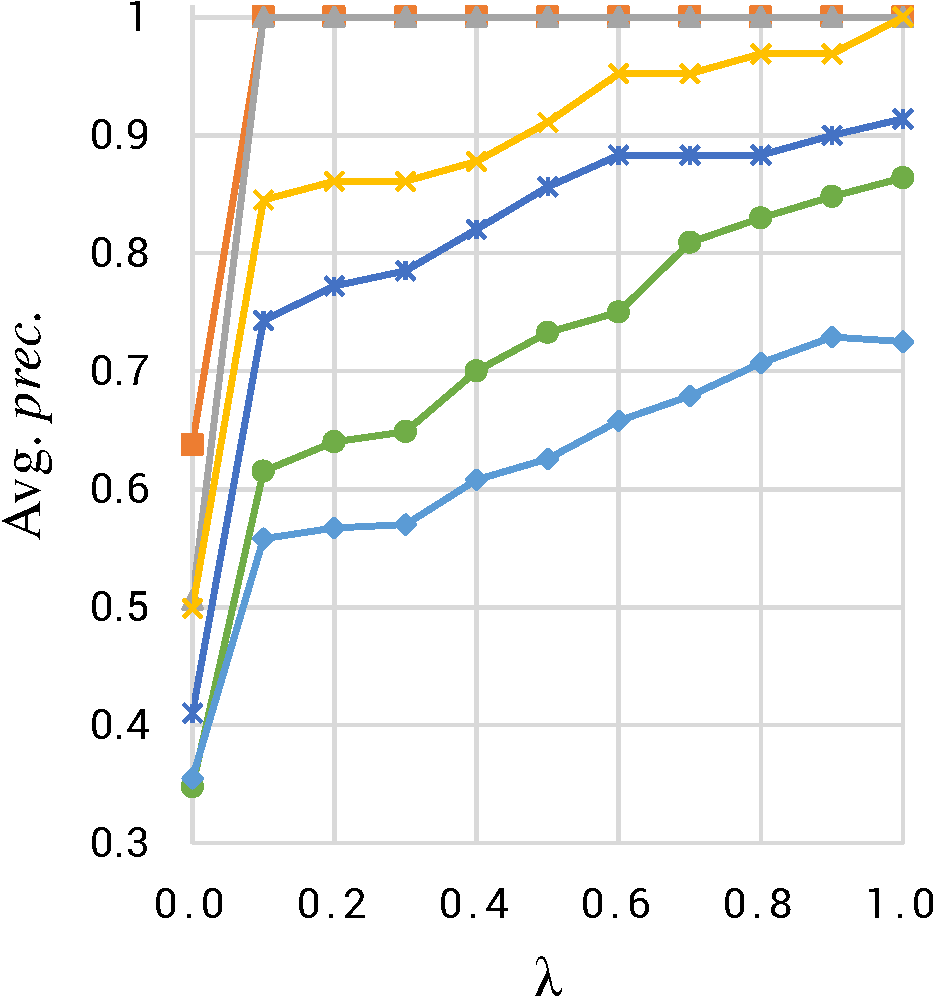
\includegraphics[width=0.5\textwidth]{figures/fb15k_ssp_pca-crop.pdf} }}    
%    \caption{Average prediction score of some top rules on FB15K dataset with the hybrid rule quality scoring function.}
%    \label{fig:fb15k}
% \end{figure}
%
%\begin{figure}[t]
%    \centering
%    \subfloat[Confidence + TransE]{{\includegraphics[width=0.5\textwidth]{figures/wiki44k_transe_conf-crop.pdf} }}
%    \subfloat[Confidence + SSP]{{\includegraphics[width=0.5\textwidth]{figures/wiki44k_ssp_conf-crop.pdf} }}\\
%    \subfloat[PCA Confidence + TransE]{{\includegraphics[width=0.5\textwidth]{figures/wiki44k_transe_pca-crop.pdf} }}
%    \subfloat[PCA Confidence + SSP]{{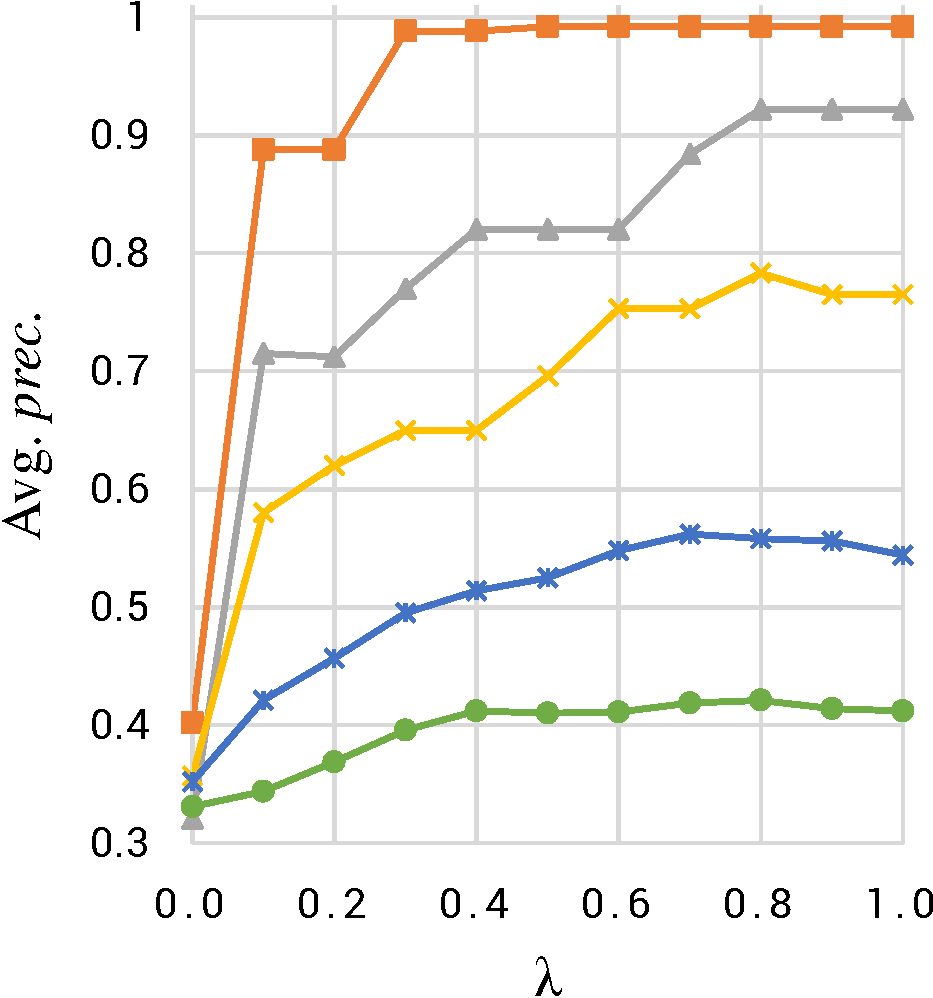
\includegraphics[width=0.5\textwidth]{figures/wiki44k_ssp_pca-crop.pdf} }}    
%    \caption{Average prediction score of some top rules on Wiki44K dataset with the hybrid rule quality scoring function.}
%    \label{fig:wiki44k}
%\end{figure}



%The higher the prediction score is, the better the rule is. Figures \ref{fig:fb15k} and \ref{fig:wiki44k} demonstrate the average prediction score of top $k$ rules on FB15K and Wiki44K datasets when using hybrid quality with different traditional rule-based measures and values of embedding weights $\lambda$. We can see that with each top $k$ rules, their average prediction score rises along with the increasing of parameter $\lambda$ until reaching some optimal value, then falls down until $\lambda$ is equal to 1. Hence, the combination of $q_{rm} $ and $q_{es}$ is crucial to achieve the best result. In addition, the hybrid quality works better than the traditional PCA confidence with every value of $\lambda$. The reason is that our training KG $\cG$ is randomly sampled that break the assumption made by PCA confidence. 













\chapter{Conclusion}
\label{chap:conclusion}
\section{Thesis Summary}
Knowledge graphs capture information about the real world and play an important role in various information systems. However, due to the automatic construction, KGs are usually incomplete so that a large amount of research effort has been committed to address this problem.

Solutions for the KGs completion problem often fall into the two categories: \textit{embedding-based} approach and \textit{rule-based} approach. In this thesis, we have presented a hybrid approach for learning non-monotonic rules from KGs that dynamically exploits feedback from a precomputed embedding model. Our method is general in that any embedding model can be utilized including text-enhanced ones, which indirectly allows us to harness unstructured web sources for rule learning. We evaluated our approach with various configurations on real-world datasets and observed significant improvements over state-of-the-art rule learning systems.
\section{Future Research Directions}
Regarding our approach, several prominent research directions could be considered to further advance this work. In what follows, we discuss the most important ones.
\subsection{Incorporation of other embedding models}
Currently, we are supporting only 3 embedding models namely TransE, HolE and SSP. While TransE and HolE models work based only on the given KG, SSP model provides the integration of entity descriptions. However, a variety of other embedding models exist that can even support different types of external data such as temporal knowledge and general Web-texts. These embedding models are more advanced and might produce better predictions than the ones that we exploited. Hence, injecting better embedding models is a promising direction for further facilitation of practicability of our approach.

\subsection{Incorporation of multiple heterogeneous external sources}
In this work, we currently rely on only a single external source, which is an embedding model. However, other types of external sources could be likewise taken into account to improve the quality of our approach. Technically, our external quality function $\mu_2$ is computed based on facts predicted by a given rule. One idea regarding the extension of our rule learning method is to exploit different external sources depending on the rule head predicate to quantify the rule quality.
Here, several possibilities exist:

\noindent- First, since the performance of different embedding models varies for different predicates \cite{Bordes:NIPS2013}, we can use the embedding models to assess only selected relations on which they perform well.

\noindent- Second, by separating relations, we can even combine the unsupervised and supervised learning settings. For instance, besides using embedding models for the relations on which they do perform well, we can also involve human judgement for other relations that are problematic for embedding models. Note that, naturally when using human inspection, the probabilistic fact assessment function $f$ would return binary values $\{0,1\}$.

\noindent- Third, different external sources could be incorporated for learning rules from general KGs, which contain relations from various domains. In particular, when learning rules from a KG with different predicates, the external quality function $\mu_2$ could be computed per predicate independently by using models trained with different domain-specific external data. For example, for movie-related predicates, IMDB could be invoked, whereas for sport-related ones, we can use data from dedicated sport websites. However, the challenge here is to figure out how to integrate these external sources to extend our hybrid probabilistic function $f$.

Incorporating many external sources can certainly improve the quality of the learned rules. However, this likely comes with the price of the increased running time and possibly memory overload. So, finding the tradeoff between these two aspects is an important point for further research.

\subsection{Auto-tuning embedding weight value}
As our experiments demonstrate, the value of the embedding weight $\lambda$ is crucial for achieving good results with our approach. Within this thesis, the best value of $\lambda$ has been empirically determined for every considered embedding model. Manually choosing a suitable value of $\lambda$ for an arbitrary dataset and embedding model requires a lot of human efforts. Hence, a relevant extension of our work concerns the development of an automatic procedure for computing the optimal weight $\lambda$. Naive strategy here would be to automate the procedure executed in Experiment \ref{exp:1}. However, other advanced and less costly solutions should exist.

Additionally, following the idea of treating every rule predicate individually as mentioned before, one can even automatically learn different values of $\lambda$ per predicate.

\subsection{Incorporation of various classical rule measures}
In this thesis, we considered \textit{standard confidence}, \textit{PCA confidence} and \textit{conviction} as classical rule measures. However, there are more sophisticated rule measures $\mu_1$ that could be also studied empirically, e.g., \textit{soft confidence} \cite{rdf2rules}, \textit{completeness-aware} measures \cite{carl}, \textit{RC confidence} \cite{measureskg}, etc. However, the challenge here is to choose the metric which is the most suitable for the dataset. For instance, \textit{PCA confidence} only performs well if the KG follows the Partial Closed-world Assumption, \textit{soft confidence} requires $type$ information to be available in the KG, and \textit{completeness-aware} measures ask for extra (in-)completeness meta-data about the KG in form of cardinality statements.

\subsection{Iterative improvement of rules and embedding model}
As mentioned in Section \ref{related_work:combine}, a variety of approaches introducing embedding models that make use of prespecified rules have been provided in the literature. So, if we plug these embedding models in our approach, an iterative improvement of rules and embedding models could be developed as sketched follows. We start with some rules extracted from a rule mining system (e.g., our system with $\lambda = 0$). Then, these initial rules are used to train the embedding model. Repeatedly, rules are then revised using our approach and rely on the trained model, which results in an iterative procedure.

\subsection{Inference of facts from intersection of rules and external source}
Currently, the main output of our approach is rules. In highly incomplete KGs, the precision of rules is normally rather low, which leads to the incorrectness of inferred facts. To tackle this issue, one could learn more complex rules (e.g., with more atoms), which could improve the likelihood of predicted facts by pruning low quality branches. However, overcoming the barrier of language bias is not easy in this context.

An alternative solution is to infer facts based on the intersection of predictions between the rules and the external source. For example, we could predict a fact as being true only if the external source gives it a probability value $f$ above a pre-defined threshold, and at the same time, the fact is binded with some rule that is confident enough. The main drawback of this method is that, while precision of predicted facts obviously increases, their recall could decrease significantly. Hence, computing the optimal thresholds is the main challenge of this research direction, which is quite interesting to study.

% \section{Conclusions}

% Advances in Information Extraction have led to the construction of large KGs in the form of \textit{$\langle$subject predicate object$\rangle$} triples. However, due to the automatic construction, these KGs can be incomplete. Horn rule mining is a popular approach to address this issue~\cite{ref10}.

% In this thesis we have looked at the problem of enhancing the quality of positive rules and subsequently improving the accuracy of their predictions, by revising the mined rules into the nonmonotonic ones. We follow the ideas from~\cite{ref12} where the same problem was studied for KGs containing only unary facts. Meanwhile, RUMIS tool implemented in our research generates nonmonotonic rules from KGs in their original format.

% We have extended the results from~\cite{ref12} to KG revision in their original relational form and developed the RUMIS system, for learning nonmonotonic rules in KGs under the OWA. Subsequently, the chosen revisions are exploited to extend the original data, and thus, they are suitable for tackling the KG completion problem. Some experiments in the thesis are conducted for testing quality of rules generated by RUMIS and the results demonstrate that the proposed approach outperforms the state of the art KG rule learning systems w.r.t. to the quality of the made predictions.

% \section{Future Directions}

% We now discuss possible future directions.

% \begin{itemize}
% \item \textbf{Tackle language bias challenge.} In this work we have fixed the language bias of the rules to be mined. Certainly, a promising and natural direction is to extend our results to further rule forms and make the language bias more flexible. The language bias can be manually specified by users, which should make the RUMIS system less restrictive and diversify possible revisions. Another possible future direction is to consider existential operators in the heads of the positive rules, e.g., \textit{$\exists$ Y hasParent(X, Y) $\leftarrow$ person(X)}.
% \item \textbf{Enriching exception forms.} Currently RUMIS only supports one exception in the body and this exception is the relation between variables in the head or a unary atom. To extend the form of nonmonotonic rules, we can increase the number of exceptions in the body of the revision. E.g., an interesting rule like \textit{isCitizenOf(X, Y) $\leftarrow$ bornIn(X, Y), not manager(X), not isAsiaCountry(Y)} could then be mined.
% \item \textbf{Optimizations.} Due to the large size of the KGs, data indexing is a time burden step in our implementation. Thus, a natural optimization direction is to store the facts in a database and to build a web service for finding results of conjunctive relational queries. Thanks to this technique, we will only build the service once at the beginning, and the data indexing step will not be necessary for every execution of the RUMIS system. Hence, the total time of the experiment should be significantly reduced.
% \item \textbf{Try more rule measures.} Other predictive measures and exception evaluation methods can be tested to search for interesting nonmonotonic rules. A survey in~\cite{ref46} specifies a variety of choices for predictive rule measures, where conviction is only one of them.
% \item \textbf{N-ary facts.} In YAGO and IMDB datasets, the facts are three-dimensional, i.e., each of them contains a subject, a predicate and an object. The Wikidata Football dataset exploited in the experiments has the same property, i.e., it is extracted from simplified version of original Wikidata where all facts are projected to three-dimensional space. One possible future extension would be to take the n-ary facts, i.e., facts containing n-parameters, into consideration. E.g., the five-dimensional fact \textit{$<$Ronaldo$>$ $<$playsFor$>$ $<$Manchester United$>$ $<$in$>$ $<$2008$>$} may appear in the full Wikidata KG.
% \item \textbf{Training KG random sampling.} In our current experiment, every learning KG is chosen from the ideal KG by removing 20\% of facts for each binary predicate. This setting is a bit restrictive, because it tries to maintain the distribution of facts over the predicates. It is worth testing the quality of predictions generated by RUMIS if the training data is chosen randomly by varying the percentage of the retained facts for every relation.
% \item \textbf{Optimize DLV.} DLV running time is a burden in the current system. Indeed, for very large KGs and 10 revised rules, it takes up to days to produce predictions. Since completing a given KG is one of the main goals of the tool, optimizations of the DLV tool should be studied to make sure that the total run time performance is acceptable.
% \item \textbf{Facts with probability.} For our experiment, the facts in the given KG are always true, which is not always the case, where some facts might be totally wrong. Indeed, modern KGs might contain incorrect triples, since their large parts are constructed automatically by information extraction techniques. As a possible future direction, probability can be assigned to facts in the training KG as the weight, and taken into account during the rule learning and revision. This will result in new predictions with confidence weights assigned to them.
% \end{itemize}

%\chapter{Appendix\\RuLES - Rules Learning with Embedding-based Support\\How to Use}
\label{chap:system}

% RUMIS stands for Nonmonotonic Rule Mining System which is a tool developed within the current thesis. The RUMIS system aims at revising Horn rules to nonmonotonic ones under the OWA. This chapter describes in details the practical implementation of the theory framework presented in Chapter~\ref{chap:frame} and uses background definitions in Chapter~\ref{chap:back}. First, we present the system overview. Second, the implementations of main components of the system are described. Finally, we discuss the system usage.

% \section{System Overview}
% \label{sec:overview}

% \begin{figure}[h]
% \centering
% \includegraphics[width=0.81\textwidth]{figures/system_overview}
% \caption{Components of RUMIS}
% \label{system_overview}
% \end{figure}

% There are six components in RUMIS as presented in Figure~\ref{system_overview} with arrows indicating the data flow from input to output. RUMIS mines the nonmonotonic rules from the original graph in the following steps:

% \begin{itemize}
% \item In (1), a KG $\cG$ is passed to RUMIS as input. It is then stored and indexed by Component 1 which is exploited to speed up the computation in the next steps.
% \item In (2), Horn rules are mined by Component 2 from facts indexed into RUMIS.
% \item In (3), normal and abnormal instance sets are found by Component 3 based on the KG $\cG$ and the Horn rules mined in the previous step.
% \item Given normal and abnormal sets known for each Horn rule, (4) represents the step of finding exception witness sets in Component 4.
% \item In (5) and (6), exception candidates are ranked in Component 6 using a measure provided by Component 5. RUMIS allocates a separate component for measure plugin to enable flexibility of ranking criteria.
% \item In (7), RUMIS returns the best revision for the Horn ruleset as output.
% \end{itemize}

% \section{Implementation}

% In this section, the main components mentioned in Section~\ref{sec:overview} are described in details.

% \subsection{Data Indexing}
% \label{data_indexing}

% \begin{figure}[h]
% \centering
% \includegraphics[width=1\textwidth]{figures/data_indexing}
% \caption{RUMIS Data Indexer}
% \label{data_indexing}
% \end{figure}

% Since the KG $\cG$ can be large, computation of (ab)normal instances as well as exception witness sets is time-consuming. To overcome this issue, data indexing is exploited. In a traditional search engine setting, terms such as words, n-grams are indexed into the system and their corresponding posting lists~\cite{ref47} are a collection of documents containing them. We exploit the same intuition in our work. More specifically, RUMIS treats every fact as a document and the terms are subjects, predicates, objects or combinations of them.

% For example, Figure~\ref{data_indexing} presents the data indexed from part of a KG in Figure~\ref{fig1.1}. Hence, given the predicate \textit{isMarriedTo}, one can determine a set of subject-object pairs corresponding to it, i.e., \textit{$<$Brad, Ann$>$} and \textit{$<$John, Kate$>$}. Similarly, given a subject and a relation, the set of objects can be retrieved. For example, we can get ``Berlin" from the question ``Where does Ann live" based on the data indexing model in Figure~\ref{data_indexing}. In this example, we index the combination of subject and predicate \textit{$<$Ann, livesIn$>$} to efficiently retrieve the result \textit{Berlin}. More formally, the Data Indexing provides the following functions that are exploited in the rest of the components:

% \begin{itemize}
% \item \textit{getPredicateSubjectSet($\cG$, object)} returns a set of predicate-subject pairs corresponding to a given \textit{object} in the KG $\cG$.
% \item \textit{getPredicateSet($\cG$, subject, object)} returns a set of predicates corresponding to the input \textit{subject, object} entities.
% \item \textit{getSubjectSet($\cG$, predicate, object)} retrieves a set of subjects for a given \textit{predicate} and an \textit{ object}.
% \item \textit{getSubjectObjectSet($\cG$, predicate)} outputs a set of \textit{subject-object} pairs for a given \textit{predicate}.
% \end{itemize}

% \subsection{Positive Rule Mining}

% \IncMargin{1.5em}
% \begin{algorithm}[h]
% \DontPrintSemicolon
% \SetAlgoLined
% \SetKwInOut{Input}{Input}\SetKwInOut{Output}{Output}
% \Input{KG $\cG$}
% \Output{Set of positive rules of the form \textit{h(X, Z) $\leftarrow$ p(X, Y), q(Y, Z)}}
% \BlankLine
% $absSupp \leftarrow \{\}$\\
% \BlankLine
% \ForEach{Triple $YqZ$ in $\cG$} {
%     \BlankLine
% 	$pXSet \leftarrow getPredicateSubjectSet(\cG, Y)$\\
% 	\ForEach{$pX$ in $pXSet$} {
% 		$hSet \leftarrow getPredicateSet(\cG, X, Z)$\\
% 		\ForEach{$h$ in $hSet$} {
% 			$absSupp[hpq]++$\\
% 		}
% 	}
% }
% \BlankLine
% Sort $hpq$ in a decreasing order of $absSupp[hpq]$\\
% \Return $absSupp$\\
% \caption{Positive Rule Mining}
% \label{algo1}
% \end{algorithm}
% \DecMargin{1.5em}

% Positive Rule Mining component computes a set of rules of the form \textit{h(X, Z) $\leftarrow$ p(X, Y), q(Y, Z)}, whose \textit{absolute support} exceeds a given threshold. Existing tools from the literature can be exploited for this component, however, due to technical issues we have re-implemented the Horn rule learning based on Algorithm~\ref{algo1}. The steps of this algorithm are described as follows. First, \textit{absSupp} defined in line 1 is initialized for storing the absolute support of patterns. In the loop (2), for each triple \textit{$<$Y q Z$>$} from the KG $\cG$, using the \textit{getPredicateSubjectSet} function in the Data Indexing component, a set of pairs \textit{X, p} is found in (3) such that \textit{$<$X p Y$>$} is in $\cG$. Then, from line 5 to 6, with \textit{X, Z} found in the previous step, RUMIS searches for every relation $h$ s.t. \textit{$<$X h Z$>$} is in $\cG$. At this point, it is guaranteed that \textit{h(X, Z), p(X, Y), q(Y, Z)} holds. After that, in line 7, the absolute support of the considered rule is increased by $1$. Finally, all rules are sorted in decreasing order of their absolute support (line 11).

% \subsection{Normal and Abnormal Set Mining}

% \IncMargin{1.5em}
% \begin{algorithm}[h]
% \DontPrintSemicolon
% \SetAlgoLined
% \SetKwInOut{Input}{Input}\SetKwInOut{Output}{Output}
% \Input{KG $\cG$, $h$, $p$, $q$ predicates in the rule \textit{h(X, Z) $\leftarrow$ p(X, Y), q(Y, Z)}}
% \Output{Normal and abnormal sets of the rule \textit{h(X, Z) $\leftarrow$ p(X, Y), q(Y, Z)}}
% \BlankLine
% $NS \leftarrow \{\}$\\
% $ABS \leftarrow \{\}$\\
% $YZSet \leftarrow getSubjectObjectSet(\cG, q)$\\
% \BlankLine
% \ForEach{Pair $YZ$ in $YZSet$} {
%     \BlankLine
% 	$XSet \leftarrow getSubjectSet(\cG, p, Y)$\\
% 	\ForEach{$X$ in $XSet$} {
% 	\uIf{$XhZ$ is in $\cG$} {
% 		Add $XZ$ to $NS$\\
% 	}
% 	\uElse {
% 		Add $XZ$ to $ABS$\\
% 	}
% 	}
% }
% \BlankLine
% \Return $NS$ and $ABS$\\
% \caption{Normal and Abnormal Set Mining}
% \label{algo2}
% \end{algorithm}
% \DecMargin{1.5em}

% This component computes normal and abnormal instance sets for a given rule and a KG as described in Algorithm~\ref{algo2}. First, in lines 1 and 2, variables for (ab)normal sets are initialized. Second, for each pair \textit{Y, Z} s.t. \textit{$<$Y q Z$>$} is in $\cG$, a set of $X$ for which \textit{$<$X p Y$>$} is in the KG is found based on the Data Indexing component (line 3 to 5). At this point, it is guaranteed that \textit{X, Y, Z} satisfy the body of the given rule. Finally, for every $X$ found in the previous step, we verify whether \textit{$<$X h Z$>$} is in the KG or not. If it is in $\cG$, then \textit{$<$X Z$>$} is added to the normal set, otherwise it is added to the abnormal set.

% \subsection{Exception Witness Set Mining}

% \IncMargin{1.5em}
% \begin{algorithm}[h]
% \DontPrintSemicolon
% \SetAlgoLined
% \SetKwInOut{Input}{Input}\SetKwInOut{Output}{Output}
% \Input{KG $\cG$, $h$, $p$, $q$ predicates of the rule \textit{h(X, Z) $\leftarrow$ p(X, Y), q(Y, Z)}}
% \Output{Exception witness set of the rule \textit{h(X, Z) $\leftarrow$ p(X, Y), q(Y, Z)}}
% \BlankLine
% $NS \leftarrow getNormalSet(\cG, h, p, q)$\\
% $ABS \leftarrow getAbnormalSet(\cG, h, p, q)$\\
% $EWS^+ \leftarrow \{\}$\\
% $EWS^- \leftarrow \{\}$\\
% \BlankLine
% \ForEach{Pair $XZ$ in $ABS$} {
% 	$pSet \leftarrow getPredicateSet(\cG, X, Z)$\\
% 	$EWS^+$ $\leftarrow$ $EWS^+$ $\cup$ $pSet$\\
% }
% \ForEach{Pair $XZ$ in $NS$} {
% 	$pSet \leftarrow getPredicateSet(\cG, X, Z)$\\
% 	$EWS^-$ $\leftarrow$ $EWS^-$ $\cup$ $pSet$\\
% }
% $EWS$ $\leftarrow$ $EWS^+$ $\setminus$ $EWS^-$\\
% \Return $EWS$\\
% \caption{Exception Witness Set Mining}
% \label{algo3}
% \end{algorithm}
% \DecMargin{1.5em}

% We now describe the algorithm for exception witness set construction (Algorithm~\ref{algo3}). Given a KG and a positive rule, this component computes all unary and binary exception candidates. To simplify the presentation, Algorithm~\ref{algo3} focuses only on computing binary exceptions, analogously, unary ones can be mined. More specifically, our goal is to find exceptions of the form \textit{e(X, Z)} which are then inserted into the body of \textit{h(X, Z) :- p(X, Y), q(Y, Z)} to get its revised rule \textit{h(X, Z) :- p(X, Y), q(Y, Z), not e(X, Z)}. Algorithm~\ref{algo3} proceeds as follows. First, normal and abnormal instance sets are found in line 1 and 2 by exploiting Algorithm~\ref{algo2}. Second, the variables $EWS^+$ and $EWS^-$ which store a set of relations between \textit{$<$X Z$>$} in the abnormal and normal sets respectively are created (line 3 and 4). Third, for every pair \textit{$<$X Z$>$} in the abnormal set, all relations between \textit{X} and \textit{Z} are added to the $EWS^+$ (line 5 to 8). After that, a similar procedure is applied to $EWS^-$ in lines 9 to 12. Finally, exception witness set $EWS$ is constructed as the difference between $EWS^+$ and $EWS^-$ (line 13), which forms the output of the algorithm in line 14.

% \subsection{Measure Plugin}

% The RUMIS system is supplied with the measure plugin which allows the user to conveniently specify various rule quality criteria. In the current implementation, confidence and conviction are supported. While the former is well-suited for descriptive purposes, the latter is accepted as a possible measure for estimating rule's predictive capabilities~\cite{ref46}. Since the main concern of this thesis is the Horn rule revision and subsequent application of the revised set for predicting possibly missing facts in the original KG, the conviction is the most suitable measure, which has thus been implemented within the RUMIS system.

% \subsection{Exception Ranking}
% \label{intuition_er}

% \begin{figure}[t]
% \centering
% \includegraphics[width=1.0\textwidth]{figures/ranking}
% \caption{(Ordered) Partial Materialization Ranking}
% \label{pm_ranking}
% \end{figure}

% \IncMargin{1.5em}
% \begin{algorithm}[h]
% \DontPrintSemicolon
% \SetAlgoLined
% \SetKwInOut{Input}{Input}\SetKwInOut{Output}{Output}
% \Input{KG $\cG$, set of positive rules $\cR_{H}$}
% \Output{Set of best revisions $R_{NM}$ for the given positive rules $R_H$}
% \BlankLine
% $R_{NM} \leftarrow \{\}$\\
% \BlankLine
% \ForEach{Rule $r$ in $R_H$} {
% 	$\cG' \leftarrow \cG$\\
% 	\ForEach{Rule $r''$ in $R_H$, $r''$ is different from $r$} {
% 		Generate safely predicted facts of $r''$ w.r.t. $\cG$ then index these facts to $\cG'$\\
% 	}
% 	Rank exceptions of $r$ based on $\cG'$, choose $r'$ as the best revision of $r$\\
% 	Add $r'$ to $R_{NM}$\\
% }
% \Return $R_{NM}$\\
% \caption{PM Ranking}
% \label{bf_pm_ranking_algo}
% \end{algorithm}
% \DecMargin{1.5em}

% We now describe the exception ranking procedure in details which is illustrated in Figure~\ref{pm_ranking} on the PM ranker.

% \begin{itemize}
% \item From a given KG $\cG$ and a set of Horn rules, EWS mining (Algorithm~\ref{algo3}) is executed to find exception candidates for each Horn rule in (1). As shown in Figure~\ref{pm_ranking}, a Horn rule may have several exceptions.
% \item (2) shows that revisions with exceptions (rules $r3, r4, r5, ...$) are used to infer new facts from the original KG.
% \item $\cG'$, i.e., the original KG $\cG$ with new predicted facts, is exploited to rank exceptions for each Horn rule in (3). The combination of steps (2) and (3) describes the interaction of different rules, i.e, facts generated by other revisions are taken into account to measure quality of a particular nonmonotonic rule.
% \item (4) reflects the process in which exceptions are ranked by Component 5 according to $\cG'$ from (3), and the best exception is chosen for the addition to the final revision set.
% \end{itemize}

% \textbf{PM ranking.} Algorithm~\ref{bf_pm_ranking_algo} describes PM ranking procedure, which takes as input a KG and a set of positive rules $R_H$ and outputs a set $R_{NM}$ of their revisions. In line 1, a set of revised rules is initialized as an empty set. After that, for each positive rule $r$ in $R_H$, we clone the original KG $\cG$ to a new KG $\cG'$. Then all other rules in $R_H$ are exploited to generate their safely predicted facts which are subsequently added to $\cG'$ (line 2 to 6) by Data Indexing component. Next, in lines 7 and 8, based on the new KG $\cG'$, exceptions of $r$ are ranked and the best revision is added to $R_{NM}$. Finally, we return $R_{NM}$ as an output of the algorithm.

% \textbf{OPM ranking.} This function is similar to PM ranking. The major difference is the way how the rules are selected for KG expansion. At the initial step, Horn rules are sorted in decreasing order of conviction measure. After that, only safely predicted facts from previous rules are exploited to assess the quality of a given rule $r$. In the OPM ranking, the order of Horn rules matters, i.e., the higher is the conviction of a Horn rule, the more prominent is its impact on other rules.

% %\IncMargin{1.5em}
% %\begin{algorithm}[H]
% %\DontPrintSemicolon
% %\SetAlgoLined
% %\SetKwInOut{Input}{Input}\SetKwInOut{Output}{Output}
% %\Input{KG $\cG$, set of positive rules $\cR_{H}$}
% %\Output{Set of best revisions $R_{NM}$ for the given positive rules $R_H$}
% %\BlankLine
% %$\cG' \leftarrow \cG$\\
% %$R_{NM} \leftarrow \{\}$\\
% %Sort all rules in $R_H$ according to the decreasing order of conviction\\
% %\BlankLine
% %\ForEach{Rule $r$ in $R_H$} {
% %	Rank exceptions of $r$ based on $\cG'$, choose $r'$ as the best revision of $r$\\
% %	Add $r'$ to $R_{NM}$\\
% %	Generate safely predicted facts of $r$ w.r.t. $\cG$ then index these facts to $\cG'$\\
% %}
% %\Return $R_{NM}$\\
% %\caption{OPM Ranking}
% %\label{opm_ranking_algo}
% %\end{algorithm}
% %\DecMargin{1.5em}

% \section{Optimization}

% \IncMargin{1.5em}
% \begin{algorithm}[h]
% \DontPrintSemicolon
% \SetAlgoLined
% \SetKwInOut{Input}{Input}\SetKwInOut{Output}{Output}
% \Input{KG $\cG$, set of positive rules $\cR_{H}$}
% \Output{Set of best revisions $R_{NM}$ for the given positive rules $R_H$}
% \BlankLine
% $\cG' \leftarrow \cG$\\
% $R_{NM} \leftarrow \{\}$\\
% \BlankLine
% \ForEach{Rule $r$ in $R_H$} {
% 	Generate safely predicted facts of $r$ w.r.t. $\cG$ then index these facts to $\cG'$\\
% }
% \BlankLine
% \ForEach{Rule $r$ in $R_H$} {
% 	Generate safely predicted facts of $r$ w.r.t. $\cG$ then remove these facts' indexes from $\cG'$\\
% 	Rank exceptions of $r$ based on $\cG'$, choose $r'$ as the best revision of $r$\\
% 	Add $r'$ to $R_{NM}$\\
% 	Generate safely predicted facts of $r$ w.r.t. $\cG$ then index these facts to $\cG'$ (reverses step in line 7)\\
% }
% \Return $R_{NM}$\\
% \caption{PM Ranking}
% \label{pm_ranking_algo}
% \end{algorithm}
% \DecMargin{1.5em}

% In Algorithm~\ref{bf_pm_ranking_algo}, the KG $\cG$ cloning and indexing procedures of the safely predicted facts are executed $|R_H|$ and $|R_H|^2$ times, respectively. Since the number of facts in $\cG$ and positive rules can be large, these operations are time-consuming. We now discuss possible optimizations of Algorithm~\ref{bf_pm_ranking_algo}, which concern the KG cloning and data indexing operations. In Algorithm~\ref{pm_ranking_algo}, we present possible refinements of Algorithm~\ref{bf_pm_ranking_algo} for the PM ranking.

% In lines 1 and 2 of the Algorithm~\ref{pm_ranking_algo}, we clone the original graph $\cG$ to $\cG'$ and create an empty nonmonotonic ruleset $R_{NM}$. After that, from line 3 to 5, for every Horn rule $r$ in $R_H$, its safely predicted facts are added to $\cG'$ using the Data Indexing component.

% Now RUMIS is ready to refine PM ranking. In line 7, for each Horn rule $r$, indexes of its safely predicted facts are removed from $\cG'$. This step is needed in order to make sure that safely predicted facts of all other rules apart from $r$ are exploited to determine the quality of $r$ (line 8). This witnesses that the interaction between nonmonotonic rules is taken into consideration during the ranking. After that, the best revision of $r$ is added to the final result in line 9. Line 10 shows a step that reverses what is done in line 7, i.e., safely predicted facts of the rule $r$ based on $\cG$ are added to $\cG'$ again. This guarantees that the same state in the next iteration can be processed with a new rule.

% With the optimized algorithm, we only need $O(|R_H|)$ operations for indexing new predicted facts and one operation for cloning the KG. This is a significant improvement compared to the original version of the algorithm. The difference is visible in practice if the KG is large and many rules are considered.

% \section{Usage}

% RUMIS~\footnote{\url{https://github.com/htran010589/nonmonotonic-rule-mining}} is developed and currently tested in Linux, we may extend it to Windows in the future. The system requires the installation of Java 8 as well as the DLV~\footnote{\url{http://www.dlvsystem.com/html/DLV_User_Manual.html}} tool. RUMIS supports the following main tasks:

% \begin{itemize}
% \item \textit{Training data generation:} Given the ideal KG, the training KG is constructed automatically by removing 20\% of facts from $\cG$ for every binary predicate.
% \item \textit{Horn rule mining:} With the training KG, a list of Horn rules of the form \textit{h(X, Z) $\leftarrow$ p(X, Y), q(Y, Z)} can be learned exploiting Algorithm~\ref{algo1}.
% \item \textit{Nonmonotonic rule mining:} Based on the training KG, exceptions for each positive rule are ranked and the best one is chosen to generate the revision.
% \item \textit{Automatic experiment:} With the KGs $\cG$ and $\cG^i$, the experiment can be executed to measure the quality of revision sets and predict new facts from the training data.
% \end{itemize}

% In the rest of this section, we list the command line options of RUMIS and explain them in details.

% %\subsection{Setting}
% %
% %\textbf{DLV.} This tool is used to extend a KG given a set of Horn or nonmonotonic rules at hand. RUMIS exploits DLV in its experiment function, i.e, a feature of RUMIS for evaluating result.
% %
% %\textbf{Predicate Ratio and Learning KG.} RUMIS provides a function for creating a learning KG based on a predicate ratio. For example, given the KG and 0.8 as the ratio, then 80\% facts of every binary predicate are retained in the learning KG. The original KG is called the approximated ideal one.
% %
% %\textbf{Working Folder.} Working folder is a location for experiment where we have learning and approximated ideal KGs in SPO format (\textit{training.data.txt} and \textit{ideal.data.txt}, resp.), positive rule and sampled positive rule files (\textit{horn-rules.txt} and \textit{selected.horn-rules.txt}, resp.) in format~\ref{form2}. Besides, DLV binary file\footnote{\url{http://www.dlvsystem.com/files/dlv.x86-64-linux-elf-static.bin}} should be downloaded and renamed to \textit{dlv.bin} in this folder. The \textit{selected.horn-rules.txt} containing a subset of rules in \textit{horn-rules.txt}, it is only necessary if we want to revise some rules in this file.

% \textbf{Command line options.} The RUMIS system supports the following options:

% \begin{itemize}
% \item \textit{-d:} This flag enables DLV in order to extend the KG.
% \item \textit{-e=[execution function]:} This option requires a string as a function for execution. Here \textit{new, pos, neg, exp} correspond to creating a new learning KG, positve and nonmonotonic rule mining and conducting the experiment, respectively.
% \item \textit{-f=[working folder path]:} With this option, experiment folder path can be specified.
% \item \textit{-h:} Option used to retrieve the help menu of the system.
% \item \textit{-l=[KG file path]:} This requires a file path to the graph in the SPO format, which enables users to choose the learning data.
% \item \textit{-o=[predicate ratio]:} With this option, one can fix the percentage of facts to be removed for the creation of a learning KG.
% \item \textit{-p=[Horn rule file path]:} This requires a string as an Horn rule file path. Each line in this file is a positive rule in the form \textit{h(X, Z) $\leftarrow$ p(X, Y), q(Y, Z)}.
% \item \textit{-r=[ranking]:} Option allows one to specify the ranking type, i.e., 0, 1, 2 standing for Naive, PM, OPM ranking, respectively.
% \item \textit{-s:} This flag is used to enable sampling of the positive rules.
% \item \textit{-t=[number of top Horn rules]:} This requires an integer as a number of positive rules with the top absolute support that will be considered for revision.
% \end{itemize}

% \textbf{Command examples.} First of all, please download the repository\footnote{\url{https://github.com/htran010589/nonmonotonic-rule-mining}}, and then uncompress \textit{data/sample.imdb.txt.zip} to get \textit{sample.imdb.txt} file. In the next step, the repository root folder should be located: \textit{\$ cd nonmonotonic-rule-mining}. Now we are ready to present some command examples for using the RUMIS system.

% \textit{Training data generation.} A learning KG of the IMDB sample dataset can be generated with predicate ratio of 80\%: \textit{\$ java -jar rumis-1.0.jar -e=new -l=data/sample. imdb.txt -o=0.8 1$>$training.sample.imdb.txt}. The generated file \textit{training.sample.imdb.txt} stores the learning KG.

% \textit{Horn rule mining.} The following command is used for executing IMDB Horn rule mining: \textit{\$ java -jar rumis-1.0.jar -e=pos -l=data/sample.imdb.txt}. The \textit{horn-rules.txt} should be then stored in the same folder as the RUMIS jar file.

% \textit{Nonmonotonic rule mining.} The following command for executing IMDB nonmonotonic rule mining with OPM ranking can be run: \textit{\$ java -jar rumis-1.0.jar -e=neg -p=horn-rules.txt -l=data/sample.imdb.txt -r=2}. One may just want to revise top 10 Horn rules with the \textit{-t} option: \textit{\$ java -jar rumis-1.0.jar -e=neg -p=horn-rules.txt -l=data/sample.imdb.txt -r=2 -t=10}. After these commands, \textit{revised-rules.txt} in the root folder is produced, which stores the computed nonmonotonic rules.

% \textit{Automatic experiment.} The working folder can be built as a directory \textit{data/experiment/IMDB} that contains all of the following files. First, \textit{sample.imdb.txt} should be renamed to \textit{ideal.data.txt} in the directory. Second, the learning data of the ideal KG should be sampled to \textit{training.data.txt}. Third, one should generate \textit{horn-rules.txt} as an output of positive rule mining function applied to the learning data. If only some positive rules need to be revised, one can list them in \textit{selected.horn-rules.txt}. Finally, DLV binary file should be downloaded to the working directory and renamed as \textit{dlv.bin}.

% The command that executes the experiment with OPM ranking and top 10 positive rules (with DLV) is: \textit{java -jar rumis-1.0.jar -e=exp -f=data/experiment/IMDB/ -r=2 -t=10 -d 1$>$experiment.txt 2$>$log}.

% %\subsection{Usage Description}
% %
% %First of all, please download the repository\footnote{\url{https://github.com/htran010589/nonmonotonic-rule-mining}}, and then uncompress \textit{data/sample.imdb.txt.zip} to get \textit{sample.imdb.txt} file. In the next step, the repository folder should be located: \textit{\$ cd nonmonotonic-rule-mining}. Now the preparation is finished, and we are ready to describe the main features of RUMIS in details.
% %
% %\textbf{Generating Learning KG.} Please generate the learning data in the SPO format with the following command: \textit{\$ java -jar rumis-1.0.jar -e=new -l=[path to KG file] -o=[ratio] 1$>$[training KG file path]}.
% %
% %\textit{Example.} A learning KG of the IMDB sample dataset can be generated with predicate ratio being 80\%: \textit{\$ java -jar rumis-1.0.jar -e=new -l=data/sample.imdb.txt -o=0.8 1$>$training.sample.imdb.txt}. Then \textit{training.sample.imdb.txt} file is the learning KG that we want to generate.
% %
% %\textbf{Horn Rule Mining.} Please run the Horn rule mining with the following command: \textit{\$ java -jar rumis-1.0.jar -e=pos -l=[path to KG file]}. This will generate two files, \textit{horn-rules.txt} for the positive rules and \textit{horn-rules-stats.txt} with the presence of \textit{absolute support}. Both rules in two files are sorted by decreasing order of the support measure.
% %
% %\textit{Example.} Please run the following command for executing IMDB Horn rule mining: \textit{\$ java -jar rumis-1.0.jar -e=pos -l=data/sample.imdb.txt}. Two generated files horn-rules.txt and horn-rules-stats.txt can be seen in the same folder with RUMIS jar file.
% %
% %\textbf{Nonmonotonic Rule Mining.} Please run the nonmonotonic rule mining with the following command: \textit{\$ java -jar rumis-1.0.jar -e=neg -p=[path to positive rule file] -l=[path to KG file] -r=[ranking option] -t=[top Horn rules]}. Revised rules can be seen from generated result file \textit{revised-rules.txt} in the same folder with RUMIS jar file. Note that \textit{horn-rules.txt} is generated by using above Horn rule mining function, or by another software. However, RUMIS currently only supports Horn rules in format~\ref{form2}.
% %
% %The file \textit{revised-rules.txt} lists the revisions of Horn rules from \textit{horn-rules.txt} with the ranking option being specified in the command. Two main sections are presented in \textit{revised-rules.txt}, the first one describes exceptions ranked for each Horn rule and the second one lists final selected revisions. As regards the first section, Naive ranking subsection is always presented on top of the file, followed by [PM $|$ OPM] one if [PM $|$ OPM] is selected, resp.
% %
% %Every ranking subsection contains many parts separated by a blank line, each of them describes rules with exceptions. The first line of each part is a positive rule and its measure values with the format: \textit{$<$positive rule$>$ $<$Conv$>$ $<$Conf$>$}. \textit{Conv} and \textit{Conf} are abbreviations of conviction and confidence measures, resp.
% %
% %The rest of each above part is top 10 negated atoms for each Horn rule which are sorted according to the decreasing order of the positive-negative conviction (\textit{PosNegConv}) of the corresponding revision achieved by inserting the negated atom to the rule. If two revisions have the same positive-negative conviction, the one with higher conviction has a higher rank. The format for describing each negated atom with its measures is: \textit{$<$not exception$>$ $<$PosNegConv$>$ $<$Conv$>$}.
% %
% %The second section of the \textit{revised-rules.txt} lists chosen revisions for all the Horn rules. They are corresponding to the best exceptions of positive rules in the subsection of given ranking option.
% %
% %\textit{Example.} Please run the following command for executing IMDB nonmonotonic rule mining with OPM ranking: \textit{\$ java -jar rumis-1.0.jar -e=neg -p=horn-rules.txt -l=data/sample.imdb.txt -r=2}. One may just want to revise top 10 Horn rules with the \textit{-t} option: \textit{\$ java -jar rumis-1.0.jar -e=neg -p=horn-rules.txt -l=data/sample.imdb.txt -r=2 -t=10}.
% %
% %\textbf{Experiment.} First of all, please create the working folder indicated above, and then run the following command for the experiment: \textit{java -XX:-UseGCOverheadLimit -Xmx[max memory]G -jar rumis-1.0.jar -e=exp -f=[working folder] -r=[ranking] -t=[top positive rules] -d -s 1$>$experiment.txt 2$>$log} where \textit{-XX, -Xmx, -t, -d, -s} are optional. \textit{-XX} and \textit{-Xmx} are used when we want to allocate more memory for RUMIS, and, if the \textit{-t} is not used, all the rules in \textit{horn-rules.txt} are revised. Besides, \textit{-s} option should only be added to the command if we just want to care about revisions of some selected rules in \textit{selected.horn-rules.txt} file.
% %
% %The first two lines of the generated file \textit{experiment.txt} present the average conviction of selected Horn rules and their final revisions. These statistics are described in the Table 1 in the next chapter with different number of top Horn rules. Besides, the rest two parts of the file show predicates extended from the learning KG for positive and revised rules, resp. Format of every tab separated line in each part is \textit{$<$relation$>$ $<$inferred facts$>$ $<$good facts$>$ $<$other facts$>$} where \textit{inferred facts} means total number of predicted triples over the relation. Besides, \textit{good} and \textit{other facts} indicate quantity of \textit{inferred facts} that are in and not in the ideal KG, resp.
% %
% %The command outputs a file \textit{encode.txt} and a DLV subdirectory in the working folder. The former is a tab separated file that maps from entities and predicates of ideal KG to their encoded IDs. The latter provides some files as follows. First, \textit{training.data.kg} is the DLV format version of \textit{training.data.txt}. Second, files \textit{chosen.rules.[naive $|$ pm $|$ opm].txt.[pos $|$ neg].[number of top rules]} list chosen rules in encoded DLV format, i.e, DLV rule format s.t. predicated and exceptions are encoded. Third, files \textit{extension.[naive $|$ pm $|$ opm].txt.[pos $|$ neg].[number of top rules]} describe KGs extended from learning data in DLV format and corresponding rules. The terms \textit{pos, neg} correspond to positive and revised rulesets which are exploited to extend KG. Finally, For each of these, there are \textit{decode, needcheck, good, conflict} extension files which present KG in SPO format, facts not in the ideal KG, facts in the ideal KG and conflicts, resp.
% %
% %\textit{Example.} The working folder can be built as a directory \textit{data/experiment/IMDB} that contains all of the following files. First, please rename \textit{sample.imdb.txt} file to \textit{ideal.data.txt} in the directory. Second, please sample the learning data of the ideal KG file and get \textit{training.data.txt}. Third, one should generate \textit{horn-rules.txt} as an output of positive rule mining function applied to the learning data. If only some positive rules need to be revised, we can list them in \textit{selected.horn-rules.txt}. Finally, DLV binary file should be downloaded to the directory.
% %
% %The command that executes experiment with OPM ranking and top 10 positive rules (without DLV) is: \textit{java -jar rumis-1.0.jar -e=exp -f=data/experiment/IMDB/ -r=2 -t=10 1$>$experiment.txt 2$>$log}. If we want to expand memory, enable DLV and selected rule option, the following command can be used. \textit{java -XX:-UseGCOverheadLimit -Xmx300G -jar rumis-1.0.jar -e=exp -f=data/experiment/IMDB/ -r=2 -t=10 -d -s 1$>$experiment.txt 2$>$log}.

% *************** Bibliography ***************
\bibliographystyle{plain}
{\small\bibliography{bibliography/reference}}
\clearpage

% *************** Appendixes ***************
\addtocontents{toc}{\vspace{2em}}
\appendix
%\appendixpage*


% *************** Back matter ***************
%\backmatter
%\input{back.tex}

\end{document}